\documentclass[11pt,nolof,chapters]{starlink}

\stardoccategory{Starlink System Note}
\stardocinitials {SSN}
\stardocsource {ssn\stardocnumber}
\stardoctitle{The Starlink Build System}
\stardocauthors{Norman Gray, Peter W Draper, Mark B Taylor, Steven E Rankin}
\stardocnumber{78.1}
\stardocdate{11 April 2005}
\stardoccopyright{%
Copyright 2004-5, Council for the Central Laboratory of the Research Councils\\
Copyright 2007, Particle Physics and Astronomy Research Council\\
Copyright 2007, Science and Technology Facilities Council
}

\stardocabstract{ This document provides an introduction to the
  Starlink build system.  It describes how to use the Starlink
  versions of the GNU autotools (autoconf, automake and libtool), how
  to build the software set from a checkout, how to add and configure
  new components, and acts as a reference manual for the
  Starlink-specific autoconf macros and Starlink automake features.


  It does not describe the management of the CVS repository in detail,
  nor any other source maintainance patterns.


  It should be read in conjunction with the detailed build
  instructions in the \code{README} file at the top of the
  source tree (which takes precedence over any instructions in this
  document, though there should be no major disagreements), and with
  \xref{sun248}{SUN/248}{}, which additionally includes
  platform-specific notes.  }

\newcommand{\secref}[1]{Sec.~\ref{#1}}
\newcommand{\myhref}[2]{\htmlref{#2}{#1}}
\newcommand{\code}[1]{\texttt{#1}}

\begin{document}
\scfrontmatter

\chapter{Introduction}
\label{intro}

The Starlink build system consists of
\begin{itemize}

\item the Starlink CVS repository;


\item build tools, consisting of modified versions of the GNU
autotools \code{autoconf} \code{automake} and
\code{libtool};


\item configuration and bootstrap code, consisting of the
\code{starconf} system and the scripts at the top level of the
Starlink source tree; and

\item the conventions for branching and tagging which are at present
only documented in the wiki, on the pages
\url{http://wiki.starlink.ac.uk/twiki/bin/view/Starlink/BranchingPolicy}
and
\url{http://wiki.starlink.ac.uk/twiki/bin/view/Starlink/CvsTagging}
(you will currently need a wiki account to see these pages).


\end{itemize}



The repository is on the machine \code{cvs.starlink.ac.uk} -- see
\secref{starlink-cvs} for further details.


The build system is intended to cover two main cases.  Firstly, it
covers the problem of building code directly from the CVS repository,
both when building the entire software set from scratch (as during the
nightly test build for example), and when working on a development
version of a particular component, within the context of an otherwise
built software set.  This includes the problem of abiding by
long-standing Starlink conventions on documentation, auxiliary tools
and installation locations.  The build system at present is concerned
primarily with the `classic' applications, which are the large volume
of legacy Starlink code which, though it is no longer being developed,
must still be maintained and be buildable by the community.  It has no
contact with the large volume of Java code, apart from having the same
tagging and branching conventions, since the building of the Java
applications is currently completely handled by the \code{ant} system.


Each component in the CVS repository is intended to be built
separately, as opposed to being built only by a make running at the
top of the tree.  Many components require other components to be
installed, and the role of the top-level makefile is to manage these
dependencies, when it is necessary to build the entire tree from
scratch.  After a fresh CVS checkout, and presuming that any
dependencies are in place, each component in the tree should be built
with the sequence of commands
\begin{terminalv}
% ./bootstrap
% ./configure
% make
% make install
\end{terminalv}
The `install' target generated by Starlink automake installs the
component as usual, but additionally creates a manifest file which is
then installed in the \code{manifests/} subdirectory under the
Starlink installation directory.  The building of the whole tree from
scratch is described in \secref{bootstrapping}, and the procedure to
build a single component, though little more complicated than
described here, is discussed in more detail in
\secref{buildingcomponents}.  You should read both of these sections
before trying the commands above.


Secondly, the build system handles the construction of portable
source-code sets -- distribution tarballs\index{distribution} -- so
that individual components can be built by users, from source, as
straightforwardly as possible.  Since we are using the GNU autotools,
much of this functionality comes for free, and we simply have to do
the relatively small amount of configuration work required to ensure
that the source set is complete (rather than requiring non-distributed
build tools) and has clearly expressed dependencies between packages.
It is an absolute requirement that the build process for users must
consist of no more than
\begin{terminalv}
% ./configure
% make
% make install
\end{terminalv}
with the usual options available for \code{./configure} and the usual
relocations available for GNU-style makefiles.  This document does not
discuss building from a distribution tarball in any more detail than
this, since there is really very little more detail to discuss.


The system does not cover the precise mechanism by which these
tarballs are distributed to users, nor the means by which they are
informed of, or helped to satisfy, the dependencies between
components; but in generating manifests and assembling the component
dependency graph, it provides the information which such a
distribution portal would need.


In other sections of this document, we discuss the tools used to
support developing within the CVS tree, including the specific
starconf tools and an overview of the GNU autotools autoconf, automake
and libtool (\secref{tools}); we discuss the procedure for building
applications within the repository (\secref{building}); and we describe
the process of adapting a currently working package to the build
system's conventions (\secref{autoconfing}).


\section{\label{entrypoints} Quick entry-points}


The build system is intended to be a fairly integrated whole, and so
this document is intended to be read straight through, rather than act
purely as a reference manual.  However it should be fairly well
cross-referenced, and so depending on your motivations for reading
this document, there is more than one reasonable entry-point.
\begin{itemize}
\item If you want to build and install a distributed source tarball,
  then you are probably reading the wrong manual, since this one
  contains rather more information than you need.  To build the
  distribution you should not need to do more than
  \code{./configure; make; make install} -- if you do need more than
  that, that's either a bug, or there's a readme you didn't read.  If
  you need to know more about the options to \code{./configure}, then
  \code{./configure --help} should provide that.  And if you really
  want or need the gory details, then \secref{configure-script} has them
  all.

\item If you want to start building and using software from the
  repository, then start with \secref{starlink-cvs} or
  \secref{buildingcomponents} and work outwards from there.

\item If you want to add another component to the repository, then you
  are probably going to have to read quite a lot of the document, but
  \secref{autoconfingexample} and \secref{importing-thirdparty} (and indeed
  most of \secref{autoconfing}) are good places to start.

\item There are some FAQs in \secref{faqs}.

\item There is a reference for the Starlink autoconf macros in
  \secref{starconfmacros}.
\end{itemize}


\chapter{Tools}
\label{tools}

This section is concerned with the tools which make up the Starlink
build system.  There are generally very few adjustments you need to
make to the program source code (though the autotools can help you
manage such things as installation directories and platform
dependencies), and the changes you will make are to the auxiliary
files which manage the build, most prominently the \code{configure.ac}
file which organises the configuration, and the \code{Makefile.am}
file which controls generating the makefile which does the work.


The build system as a whole consists of a number of components:
\begin{description}

\item[The Starlink autotools\index{autotools!Starlink changes}] These
  consist of versions of the GNU autotools, which are part of the
  Starlink CVS repository, and which are built and installed as part
  of the top-level bootstrap.  They should be installed in
  \file{/star/buildsupport/bin}, or its equivalent if you have
  installed a set of tools in a tree other than \file{/star}.  Since
  they have been extended and customised, they are essential; you
  cannot build the Starlink collection without them.  There is an
  introduction to the autotools in \secref{tooloverview}, covering their
  interrelationships and basic usage.


  We use (at the time of writing) an unmodified libtool, a moderately
  extended autoconf, and an extended and customised automake.  The
  description below explains the use of these tools as modified; see
  \secref{gnutools} for details of the differences from the stock
  autotools.

\item[The Starlink autoconf macros\index{autoconf}] There is an
  extensive set of autoconf macros which support building Starlink
  applications.  You use these as you would any of the standard
  autoconf macros, by invoking them within the \file{configure.ac}
  file.

  The macros are described in detail in \secref{starconfmacros}.

  The autoconf program which is used is not itself customised for
  Starlink use.  Instead, the macros are installed using the standard
  autoconf extension mechanism, which uses the application
  \emph{aclocal}.  This is discussed in passing in
  \secref{tooloverview}, and we mention it only in passing here.

\item[starconf\index{starconf}] This is the program which handles
  installing required macros, and configuring your directory ready to
  use the build system.  Associated with \emph{starconf} is the
  \emph{starconf-validate} program which checks that your directory is
  configured correctly, and the program \emph{./starconf.status},
  which unpacks required files, and allows you to make the link back
  to the configuration used to build the software.  All these are
  described in detail in \secref{starconf}.

\end{description}

\section{\label{tooloverview}Overview of the Autotools}
\index{autotools}

The autotools as a group help you create software distributions which
will build reliably on a large variety of platforms.  They are most
obviously associated with unix systems, but in fact support the larger
class of POSIX systems which have an implementation of \code{/bin/sh}
available -- a class which includes Windows machines, through the
\href{http://www.cygwin.com/"}{cygwin environment}.


The minimum required contact with the autotools is to generate the
files which will let you configure a freshly checked-out directory
before working on it, since these configuration files are not checked
in to the repository.  The \code{./bootstrap} script (see
\secref{starconf}) will do this for you, but it can only do this if the
autotools are installed (see \secref{bootstrappingonly}).


The aim of the notes below is to give you an overview of autoconf and
automake functionality, enough to make it possible for you to roughly
understand the existing configuration files, and to make it easier to
approach the full autoconf and automake documentation.  We start off
with a broad overview, and provide a few further details in the
subsections which follow.


The two most obvious and important files are
\code{configure.ac}\index{configure.ac} and
\code{Makefile.am}\index{Makefile.am}.  The first tells autoconf how
to make the \code{./configure} script which does the actual
configuration work, and which will be distributed with your package,
the second (assuming you're using automake rather than
hand-maintaining the input Makefile) tells automake how to create the
template makefile \code{Makefile.in}, which is also distributed with
your package, and which is edited by the \code{./configure} script to
(finally!)  produce the \code{Makefile} which (finally!) builds the
code on the user's system.


It's useful to illustrate the inputs and outputs of the various tools.
First are autoconf and automake:

\begin{figure}[h!]
  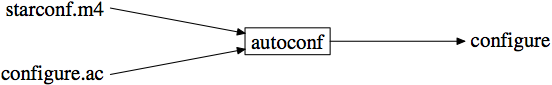
\includegraphics{ssn78-2}
  \caption{Inputs to, and outputs from, autoconf}
\end{figure}

\begin{figure}[h!]
  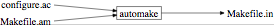
\includegraphics{ssn78-3}
  \caption{Inputs to, and outputs from, automake}
\end{figure}

As you can see, although \code{configure.ac} is most associated with
autoconf, automake reads it, too, to discover for example whether you
have invoked \code{AC\_PROG\_LIBTOOL} or \code{STAR\_MONOLITHS}, and so
whether it needs to add the appropriate support in the generated
\code{Makefile.in}.


Once the \code{./configure} script is created, it is able to
interrogate the system (the user's system, that is, not the
developer's), and based on that edit the various \code{.in} files to
produce their corresponding outputs.


\begin{figure}[h!]
  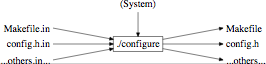
\includegraphics{ssn78-4}
  \caption{Inputs and outputs to configure}
\end{figure}

This diagram for \code{./configure} shows a file
\code{config.h.in}\index{config.h.in} being edited.  This file --
which we will have more to say about in \secref{autoconfoverview} -- is a
template list of C preprocessor definitions, which can be
\code{\#include}d in a C source file, and so used to configure the use
of functions and definitions there.  Like any of the other \code{.in}
files, it is possible to maintain this by hand, but it is more
reliable to maintain it using another application
\emph{autoheader}\index{autoheader}, which looks as follows.

\begin{figure}[h!]
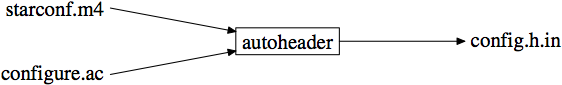
\includegraphics{ssn78-1}
\caption{Inputs and outputs to autoheader}
\end{figure}

The other file we have not mentioned yet is
\code{starconf.m4}\index{starconf!location of macros}.  This file
contains macros (in the implementation language of autoconf, m4) which
are used to extend autoconf's functionality, supplying the
Starlink-specific autoconf support.  You will not typically have
anything to do with this file, and we mention it only to indicate
schematically where (some of) the Starlink magic comes from.  This
file is not in your working directory, but is installed in the place
the autotools expect to find it, by the \emph{starconf} application
described in \secref{starconf}.  You may also notice a file
\code{aclocal.m4}\index{aclocal} in your directory.  This is a cache
of autoconf macros, maintained by the autoreconf program; it should
not be checked in.


Of the applications mentioned above, automake, autoconf and (usually
implicitly) autoheader are run on the developer's machine before or
while making a distribution; thus the products of these programs,
\code{./configure}, \code{config.h.in} and \code{Makefile.in}, are
included in the distribution, and the \code{.in} files edited by the
\code{./configure} script into the \code{config.h} and \code{Makefile}
which actually control the build.


We have elided some details here, for simplicity, and we could
possibly have elided more, since you generally don't have to concern
yourself with autoheader or \code{aclocal.m4}.  You don't even have to
worry about the dependencies between these files and applications,
since the \code{Makefile.in} which automake generates knows about
these dependencies and will generally keep things up to date for you.
If you wish to be sure things are up to date, then you can simply run
application \emph{autoreconf} (see \secref{autoreconf}), which knows
enough about the relationships between them to run each of the
required ones in the correct order.  This is likely the only one of
the autotools commands which you will run yourself.


For more details on the relationships between these applications, and
fuller diagrams, see the online copy of the book
\href{http://sources.redhat.com/autobook/}{`GNU Autoconf,
  Automake, and Libtool'}, and in particular
\href{http://sources.redhat.com/autobook/autobook/autobook_276.html}{Appendix
  C of that book, `Generated file dependencies'}.


Comprehensive details of the autotools are to be found in their
respective manuals, which are available online
at\index{autotools!documentation}

\begin{itemize}
\item \url{http://www.gnu.org/software/autoconf/manual/autoconf-2.57/autoconf.html}

\item \url{http://www.gnu.org/software/automake/manual/}

\item \url{http://www.gnu.org/software/libtool/manual.html}

\end{itemize}

The autoconf manual is relatively clear, once you have a basic idea of
what it's trying to do, but it's more effective as a reference manual
than as a tutorial.  The automake manual should be regarded as a
reference manual only: you might not guess from the manual, that
automake will make your life simpler, rather than full of anguish,
suffering and confusion.  It doesn't really matter how good or bad the
libtool manual is, since if you discover you have to look at it, you
already know your future holds pain, and the manual isn't going to
make things better or worse.



It's also worth looking at the
\href{http://www.gnu.org/prep/standards_48.html}{`Release
  Process'} section of the GNU Coding Standards document.  Though we
are not necessarily following these standards, this section both
describes what is conventional packaging in the open-source world, and
outlines the conventions which the autotools are designed to support.


\subsection{ \label{autoconfoverview} \index{autoconf!overview} Autoconf}


We use a slightly extended version of autoconf.  See
\code{autoconf --version} for the base version number.


The goal of autoconf is to help you make your program portable, by
allowing you, at build time, to adapt the program to the facilities
available on the machine on which the program is being built.


You control this through a script called \code{configure.ac} (which
was called \code{configure.in} in older versions of autoconf).  The
autoconf program produces from this a very portable \code{/bin/sh}
script called \code{configure}, which is distributed as part of your
package, and which the person building the package runs as the first
part of the \texttt{./configure; make; make install} incantation.


The \code{./configure} script probes the system it is running on,
finding compilers, testing the behaviour of the local unix system,
testing whether specific include files exist or not, testing whether
required functions are available and working as expected, and managing
some configuration by the user, such as allowing them to specify where
the package is to be installed.


This information is only useful if it can be communicated to your
program in some way.  This is done by the configure script by editing
the values of certain `substitution variables' into a list of template
files.


For example, you might have a version header file\index{version
  numbers} \code{version.h.in}, containing the line
\begin{terminalv}
const char version[] = "@PACKAGE_VERSION@";
\end{terminalv}
The configure variable \code{PACKAGE\_VERSION} is one of those
substituted by default, and if this file were listed as one of those
to be substituted (by mentioning it in the autoconf macro
\code{AC\_CONFIG\_FILES(version.h)}\index{autoconf!macros!AC_CONFIG_FILES}),
then a file \code{version.h} would be created containing the contents
of the \code{version.h.in} file with the \code{@PACKAGE\_VERSION@}
substituted by the version number declared within the \code{configure}
file.


Although this substitution process can be done for any template file,
there are two template files which are used particularly often.


The first is \code{Makefile.in}, which is a skeleton makefile which
you might write by hand (though see the discussion of automake in
\secref{automakeoverview}).  There is an example of this at the top level
of the Starlink build tree.  A typical \code{Makefile.in} might
include lines like
\begin{terminalv}
LN_S = @LN_S@
CC = @CC@
myfile.o: myfile.c
        $(CC) -o myfile.o myfile.c
\end{terminalv}
That, combined with autoconf macros \code{AC\_PROG\_CC} and
\code{AC\_PROG\_LN\_S}, would allow you to produce a file \code{Makefile}
which was customised to use the C compiler appropriate to the local
environment, and which had, in the makefile variable
\verb+{$(LN_S)+
\index{symbolic links} a command which makes links between files if
the local platform supports that, or makes hard links or simple copies
if that is all that is possible.


As well as configuring the makefile, you may also want to configure
the source code, so that you can take different actions in your code
depending on whether certain functions or headers are available.  That
is is most often done via a particular configured file, conventionally
named \code{config.h}.  This second way of communicating with your
source code has the \code{config.h} file substituted with a number of
C preprocessor \code{\#define} statements.  For example, if you
included in your \code{configure.ac} file the lines:
\begin{terminalv}
AC_CHECK_HEADERS([sys/wait.h])
AC_CHECK_FUNCS([strchr])
\end{terminalv}
then the configure script generated from that source would include a
test of whether the \code{sys/wait.h} header file was available, and
whether the \code{strchr} function was available in the C library.  If
so, the resulting \code{config.h} file would include the lines
\begin{terminalv}
#define HAVE_SYS_WAIT_H 1
#define HAVE_STRCHR 1
\end{terminalv}
Whereas most configured files are substituted as a result of being
mentioned in a \code{AC\_CONFIG\_FILES()} macro, the \code{config.h.in}
input file is configured through \code{AC\_CONFIG\_HEADERS(config.h)},
which does its configuration in a slightly different way.


After including this file into your source code with:
\begin{terminalv}
#include <config.h>
\end{terminalv}
you can adjust the compiled code with suitable \code{\#if} preprocessor
conditionals, such as
\begin{terminalv}
#if HAVE_SYS_WAIT_H
#include <sys/wait.h>
#endif
\end{terminalv}


It is possible to maintain the \code{config.h.in} file by hand, but
generally better to generate it by using the \emph{autoheader}
application which is part of autoconf.  This scans your
\code{configure.ac} and extracts into \code{config.h.in} mentions of
all those preprocessor defines it finds.  Autoheader knows about
macros such as \code{AC\_CHECK\_HEADERS} above; if you wish to add
further switches to the \code{config.h.in} file, you should do so by
calling the autoconf macro
\code{AC\_DEFINE}\index{autoconf!macros!AC_DEFINE}.  See the section
\href{http://www.gnu.org/software/autoconf/manual/autoconf-2.57/html_node/autoconf_82.html}{7.1 Defining C
  Preprocessor Symbols} in the autoconf manual for further details.
Autoheader is one of those applications run on your behalf by
autoreconf (see \secref{autoreconf}).


Note the angle brackets round \code{config.h}: this is preferred to
double quotes, as it gives the makefile the option of controlling
where the source code is; in the simplest case this is handed by
simply adding \code{-I.} to the compile line.  We don't take take
advantage of this particular flexibility, but it is a good habit to
get into.


An illustrative \code{configure.ac}\index{configure.ac!example} might
look like this (with line numbers inserted):
\begin{terminalv}
1   AC_INIT(mypack, 1.2, starlink@jiscmail.ac.uk)
2   AC_CONFIG_SRCDIR(src.c)
3   STAR_DEFAULTS
4   AC_PROG_CC
5   AC_PATH_PROG(PERL, perl)
6   AC_CHECK_HEADERS([sys/time.h])
7   STAR_MESSGEN(mypack_err.msg)
8   AC_CONFIG_HEADERS(config.h)
9   AC_CONFIG_FILES(Makefile)
10  AC_CONFIG_FILES(myscript.pl, [chmod +x myscript.pl])
11  AC_OUTPUT
\end{terminalv}


%          <!-- The media selectors below are currently at 'all': might be
%               useful to switch these back to 'screen' and add other
%               branches for other media. -->

Line 1: This line is required.  It declares the package name, version
number, and bug-report address.  Each of these is available for
substitution via the substitution variables \code{PACKAGE\_NAME},
\code{PACKAGE\_VERSION} and \code{PACKAGE\_BUGREPORT}.See autoconf
\href{http://www.gnu.org/software/autoconf/manual/autoconf-2.57/html_node/autoconf_16.html'}{4.1 Initializing
  configure}


Line 2: This is largely a sanity check, and produces an error if the
named file (in this case \code{src.c}) is not in the source directory.
The source directory is typically the current directory, but you can
specify a different one using the \code{--srcdir} option to
\code{./configure}, if you have a good reason for doing that.  See
autoconf \href{http://www.gnu.org/software/autoconf/manual/autoconf-2.57/html_node/autoconf_18.html}{4.3 Finding
  configure Input}


Line 3: This macro is one of the Starlink extensions, and the only
required Starlink macro\index{starconf!macros!STAR\_DEFAULTS}.  It sets
up the defaults required for building Starlink applications, and
assures the \code{starconf} program that it's being run in the correct
directory.  See \secref{starconf} for a description of the starconf
application, and \secref{starconfmacros} for details of the associated
macros.


Line 4: This finds a working C compiler, and prepares to substitute it
in the substitution variable \code{CC}.  Presumably the Makefile.in
has a line \code{CC=@CC@}.  See autoconf
\href{http://www.gnu.org/software/autoconf/manual/autoconf-2.57/html_node/autoconf_64.html}{5.10.3 C Compiler
  Characteristics}


Line 5: Find a binary called \code{perl} in the current \code{PATH}
and assign the substitution variable \code{PERL} the full path to it.
The most common way of using this would be for the file
\code{myscript.pl.in} to start off with the line
\begin{terminalv}
#! @PERL@ -w
\end{terminalv}
so that the script ends up with the correct full path.  See line
10<span media="all"> and autoconf
\href{http://www.gnu.org/software/autoconf/manual/autoconf-2.57/html_node/autoconf_41.html}{5.2.2 Generic Program and
  File Checks}


Line 6: check that the system has an include file \code{sys/time.h} in
the include path, and if it has, make sure that the \code{cpp}
variable \code{HAVE\_SYS\_TIME\_H} is defined.  If this were a real
configure file, you would likely have several other header tests here
(in a space-separated list, surrounded by square brackets), and cpp
branching inside your source code to handle the various cases.  See
line 8 and autoconf \href{http://www.gnu.org/software/autoconf/manual/autoconf-2.57/html_node/autoconf_51.html}{5.6.3
  Generic Header Checks}.


Line 7: Another Starlink extension.  It declares that this package has
a set of ERR messages in the given file, and that autoconf should
check the location of the messgen application.  The argument is in
fact optional (it merely causes the files to be declared as
pre-distribution files -- see \secref{macro-predist-sources}; this line
should be partnered by a declaration of the variable
\code{include\_MESSAGES} in the corresponding \code{Makefile.am}.  See
\secref{macro-messgen} for fuller details.


Line 8: This is the macro that makes cpp configuration information
available, by editing the header file \code{config.h.in} (this file
name is conventional, but not required).  See autoconf
\href{http://www.gnu.org/software/autoconf/manual/autoconf-2.57/html_node/autoconf_27.html}{4.8 Configuration Header
  Files}. If you want to put extra information into this file, use the
\code{AC\_DEFINE}\index{autoconf!macros!AC_DEFINE} macro: a declaration
like \code{AC\_DEFINE(SPECIALCASE,1)} would insert
\code{\#define SPECIALCASE 1} into the \code{config.h}; autoheader also
spots this and puts a suitable template into \code{config.h.in}.  See
the autoconf manual, section
\href{http://www.gnu.org/software/autoconf/manual/autoconf-2.57/html_node/autoconf_82.html}{Defining C preprocessor
  symbols}, for further details.


Line 9: This does the work of substituting the results of the various
tests into the files being configured.  For each of the files named in
the (space-separated list) argument, which most typically includes
\code{Makefile}, autoconf expects to find a file of the same name but
with \code{.in} appended, and this is the file which has the
substitutions edited in.  (Automake also looks at this line, and if it
sees a \code{Makefile} mentioned here, it looks to see if there is a
corresponding \code{Makefile.am} already present, and if so, recurses)


Line 10: This is a variant of line 9.  The \code{AC\_CONFIG\_FILES}
macro takes a second argument consisting of one or more lines of shell
script to post-process the file in question, in this case making sure
that the generated file is executable.


Line 11: This is the line which \emph{really} does the work.See
\href{http://www.gnu.org/software/autoconf/manual/autoconf-2.57/html_node/autoconf_19.html}{4.4
  Outputting Files}.


Of this script, it is lines 1, 2 and 11 which are absolutely required,
along with something like line 9 to make the configure script do
something useful.


It is useful to think of the \code{configure.ac} file as being the
template for the final \code{./configure} script, with the autoconf
macros simply expanding to (large chunks of) shell script during
translation by the autoconf program.  This isn't the whole truth, but
it suffices for almost all purposes.  About the only place where this
view might deceive you is if you wished to modify a file after it was
generated by \code{AC\_CONFIG\_FILES} for example; if you did that
immediately after the \code{AC\_CONFIG\_FILES} line it would fail, since
the code which generates the files is in a different place from the
\code{AC\_CONFIG\_FILES} line -- that is why \code{AC\_CONFIG\_FILES} has
its second argument.  With this view it is natural that you can add
any other shell scripting to your configure.ac, adding any tests and
switches you fancy.  You communicate the results of your scripting to
the output files by making shell variables into substitution
variables, and the way you do that is by calling \code{AC\_SUBST} on
them.  Thus, after
\begin{terminalv}
wibble=''
... # lots of clever scripting
AC_SUBST(wibble)
\end{terminalv}
any occurrences of the string \code{@wibble@} in the substituted files
will be replaced by the value of \code{wibble} at the \emph{end} of
the \code{./configure} script.


\subsubsection{ \index{m4} M4 syntax and traps}

Autoconf does its work by running the \code{configure.ac} file through
the text processor GNU \code{m4}, and this can cause occasional
surprises.


M4 is a macro language, intended for very much the sort of rewriting
that autoconf does.  When m4 processes a file, anything at all that
looks like an m4 macro is substituted, so that there is no macro
invocation character like the backslash in \TeX;.  Macros can take
arguments, delimited by round brackets and separated by commas, as
illustrated above.


The first oddity is to do with comment characters.  The default m4
comment character is \code{\#}, but since this is also the shell script
and makefile comment character, autoconf makes it an ordinary
character.  Thus to add comments to a \code{configure.ac} file which
won't make it into the \code{./configure} file, you should prefix them
with the m4 \emph{macro} \code{dnl} (which means `delete to next
newline'), as in
\begin{terminalv}
dnl   This is a comment
AC_INIT(...)
\end{terminalv}
There's no harm in including \code{\#}-style comments in your
\code{configure.ac} file and allowing these to be passed through to
the output file, since `got-here' type comments can sometimes help you
debug the \code{./configure} script.


The default m4 quote characters are the left and right single quotes,
but autoconf changes these to left and right square brackets.  You
need to use these in two circumstances, firstly when you have a
multi-word argument to a macro, and particularly when that argument
contains a comma, and secondly if a piece of text looks like a current
m4 macro.  In general, if you need to care about m4 quoting rules,
you're in trouble, but see section
\href{http://www.gnu.org/software/autoconf/manual/autoconf-2.57/html\_node/autoconf\_90.html}{8.1 M4 Quotation} in the
autoconf manual, for some advice.



\subsection{\label{automakeoverview} \index{automake!overview}Automake}


The most typical use of autoconf is to configure a file
\code{Makefile.in}.  You can write this yourself, as described in
\myhref{autoconfoverview}{the discussion of autoconf}, but since so
much of a typical makefile is boilerplate, automake exists to write
this boilerplate for you.  This has the additional advantage that we
can support and enforce Starlink-specific conventions with a
customised installation of automake.  We (currently) use an adapted
version of automake -- see \code{automake --version} for the version
number, and \secref{gnutools} for a summary of the differences.


The file which controls automake is
\code{Makefile.am}\index{Makefile.am}.  Automake reads both this file
and \code{configure.ac}\index{configure.ac!and automake}, and based on
these emits a \code{Makefile.in}.  It is this latter file which you
distribute, and which is substituted at build time by the
\code{./configure} script which autoconf generates in turn.


The resulting \code{Makefile} has rules to do all the required
building and installation in a very portable fashion, as well as
targets to make distributions (\texttt{make dist}), do tests
(\texttt{make check}), clean up (\texttt{make clean}, \texttt{make
distclean} and \texttt{make maintainer-clean}) and, in the case
of Starlink automake, do an install along with an installation
manifest.


The \code{Makefile.am} script consists, in its simplest form, of a
sequence of declarations of the relationships between the source files
in your distribution and the programs and libraries they are intended
to produce.  For example, here is the \code{Makefile.am} for the PAR
library, slightly edited:
\begin{terminalv}
## Process this file with automake to produce Makefile.in

lib_LTLIBRARIES = libpar_adam.la
libpar_adam_la_SOURCES = $(F_ROUTINES)

include_HEADERS = $(PUBLIC_INCLUDES)

F_ROUTINES = \
     par1_menu.f \
     par_cancl.f \
     [blah...]

PUBLIC_INCLUDES = \
    PAR_ERR \
    PAR_PAR \
    par.h \
    parwrap.h \
    par_err.h \
    par_par.h

BUILT_SOURCES = PAR_ERR par_err.h
\end{terminalv}


Overall, you can see that this automake source file is syntactically a
makefile -- the statements in this example look like makefile variable
settings, and it is possible to put makefile rules in the
\code{Makefile.am} file, though that is not illustrated here.  This is
slightly deceptive, however, and while it was useful to think, above,
of the \code{configure.ac} file as being the template of the eventual
\code{./configure} script, for automake you should think of the match
between the input syntax and the makefile as a happy coincidence.  You
provide information to automake through the \code{Makefile.am} file,
and based on that it then emits the \code{Makefile.in} it thinks you
want (or need, at least).


The first line is a conventional comment.  It starts with a doubled
hash mark \code{\#\#}, which causes automake to discard the text after
it; lines beginning with a single comment character are copied
verbatim into the generated \code{Makefile.in}.


The next stanza declares that there is to be a library
\code{libpar\_adam.la}, and that the sources for this file are in the
`makefile variable' \code{F\_ROUTINES}.


Though the variables \code{F\_ROUTINES} and \code{PUBLIC\_INCLUDES} are
specific to this makefile, and arbitrary, the other variable names
have both structure and meaning for automake.


The variable \code{lib\_LTLIBRARIES} consists of the `prefix'
\code{lib} and the `primary'
\code{LTLIBRARIES}\index{automake!prefixes and primaries}.  The
primary tells automake that you wish to build the libtool library
\code{libpar\_adam.la}, and the prefix indicates that this is to be
installed with the other libraries (the variable
\code{pkglib\_LTLIBRARIES}, for example, would tell automake that you
wanted to install the result in a package-specific library).  For each
of the libraries listed in this variable, separated by spaces, there
must be a corresponding \code{\_SOURCES} variable, which has the
`primary' \code{SOURCES} and a prefix formed from the library name,
which lists the set of source files for that library.  The prefix must
be canonicalised by replacing with underscores everything other than
letters and numbers.  As well as declaring the files which are to be
compiled into the library, this indicates to automake that these
source files are to be distributed as part of the final tarball, and
that it must emit makefile rules to install the library in the correct
place, with the correct installation commands.  For the list of such
associated primaries, see section
\href{http://www.gnu.org/software/automake/manual/html_node/Program-and-Library-Variables.html}{Program
  and Library Variables} of the automake documentation.


By default, libtool builds both static and shared
libraries\index{shared libraries}.  You can control this if necessary
with the \code{--enable-shared} and \code{--disable-shared} options to
\code{./configure}, and with the \code{AC\_DISABLE\_SHARED} autoconf
variable.  For further details see the documentation for
\code{AC\_PROG\_LIBTOOL} in the
\href{http://www.gnu.org/software/libtool/manual.html}{Libtool
  manual}.


If we only wanted to build static libraries, we would replace this
line with \code{lib\_LIBRARIES = libpar\_adam.a}, and the given library
would be built in the usual way, without involving libtool.


The \code{LIBRARIES} and \code{LTLIBRARIES} primaries can have any one
of the prefixes \code{libdir}, \code{pkglibdir}, \code{check} or
\code{noinst}, with the latter indicating that the library should be
built but not installed.  Having non-installed libraries can be useful
when you are building a library conditionally, or in stages.  Libtool
refers to these as `convenience libraries', and they are discussed in
section
\href{http://www.gnu.org/software/automake/manual/html_node/Libtool-Convenience-Libraries.html}{Libtool
  Convenience Libraries} of the automake manual.


The other very important primary (not shown here) is \code{PROGRAMS},
which describes programs which are to be built and installed (the
special Starlink case of monoliths is described below).  This can have
the prefixes \code{bin}, \code{sbin}, \code{libexec}, \code{pkglib},
\code{check} or \code{noinst}: \code{check} is for tests, and is
described in \secref{regressiontests}; \code{noinst} indicates that
the program should be built but not installed, and is useful for
programs which are used during the build -- for generating header
files for example -- but which are not part of the final product.
There is no single standard list of prefixes, since each primary
supports only a subset of them (you cannot declare
\code{bin\_LIBRARIES}, for example), but several are mentioned in
automake's
\href{http://www.gnu.org/software/automake/manual/html_node/Install.html}{What
  Gets Installed}, and the directories in question are discussed in
autoconf's
\href{http://www.gnu.org/software/autoconf/manual/autoconf-2.57/html_node/autoconf_24.html}{4.7.2
  Installation Directory Variables}.


The \code{include\_HEADERS} line is similar: it indicates that the
listed files are to be distributed, and are to be installed in the
correct place for include files.


The final line which is significant to automake is the
\code{BUILT\_SOURCES} line\index{BUILT_SOURCES}.  This says that, even
though \code{PAR\_ERR} and \code{par\_err.h} are to be installed and
distributed, they are not actually genuine source files, but must be
built; adding the \code{BUILT\_SOURCES} line forces automake to add a
dependency for these files at an artificially early stage.  It is only
rather rarely necessary to include a line like this.  If one of the
source files were in this category, then it would naturally be built
when it was required, without any need to add it to
\code{BUILT\_SOURCES}.  As it happens, there is no rule in this file
for building these targets; that is added automatically by automake
when it spots that the \code{STAR\_MESSGEN} macro has been used in the
\code{configure.ac} file which partners this \code{Makefile.am}.  In a
more general case, however, you would add a make-style rule to the
\code{Makefile.am} file to build these files from their (presumably
undistributed) sources.  See also
\href{http://www.gnu.org/software/automake/manual/html_node/Sources.html}{Built
  sources} in the automake manual.


For a second example, we can look at the \code{Makefile.am} for the
\code{sst} application (this is a non-distributed application for
building documentation).
\begin{terminalv}
## Process this file with automake to produce Makefile.in

bin_SCRIPTS = start

bin_MONOLITHS = sst_mon
sst_mon_SOURCES = \
    sst_mon.f \
    $(sst_mon_TASKS:=.f) \
    $(SUBSRC) \
    $(SUBCSRC) \
    $(PRIVATE_INCLUDES)
sst_mon_TASKS = forstats procvt prohlp prolat propak prohtml
sst_mon_LDADD = $(LDADD) `fio_link`


SUBSRC = sst_clean.f sst_fwild.f sst_latex.f sst_puts.f  sst_trcvt.f \
         sst_cntac.f sst_get.f sst_latp.f sst_rdad1.f sst_trhlp.f \
         [blah...]

SUBCSRC = find_file.c

PRIVATE_INCLUDES = SST_PAR SST_SCB

# special installation directory (but see discussion below)
sstsupportdir = $(bindir)
sstsupport_DATA = sun.tex sst.tex layout.tex forstats.dat html.sty

# The `start' script needs to have installation locations edited into it
edit = sed \
    -e 's,@bindir\@,$(bindir),g' \
    -e 's,@VERSION\@,$(VERSION),g'
start: start.in
    rm -f start.tmp start
    $(edit) \
        -e 's,@edited_input\@,start: produced from start.in by Makefile.am,' \
        $(srcdir)/start.in >start.tmp
    mv start.tmp start

EXTRA_DIST = start.in $(sstsupport_DATA)
\end{terminalv}


This makefile configures and installs a script, builds and installs a
monolith, and adds some supporting data files in a non-standard place.


The \code{SCRIPTS} primary indicates to automake where and how to
install the \code{start} script.  The \code{start} script must be
generated, since it is to include the version number and installation
location.  Since it includes the installation location, it should
\emph{not} be generated at configure time or install time, but instead
at make time, so that the user is free to specify one installation
prefix at configure time (through \texttt{./configure --prefix=www}),
override this with another prefix at build time (through \texttt{make
  prefix=xxx}) and specify a \emph{different} one -- presumably a
staging location or something similar -- at installation time (through
\texttt{make prefix=yyy install}).  It is the prefix at \emph{build}
time that is to be baked into the code, if any such baking has to be
done.  This is one of the GNU conventions mentioned in
\secref{tooloverview}, and is discussed in a little more detail in
section
\href{http://www.gnu.org/software/autoconf/manual/autoconf-2.57/html_node/autoconf_24.html}{4.7.2
  Installation Directory Variables} of the autoconf manual.  This is
why we have to include a makefile-style rule for deriving the file
\code{start} from its template \code{start.in}.  This substitutes in
the values of the makefile variables \code{bindir} and \code{VERSION};
these get their values, in the resulting \code{Makefile}, by having
those values substituted in to the generated \code{Makefile.in} by the
generated \code{./configure} script; the careful escaping of the
@-signs in the sed command is to match the \code{@...@} in
\code{start.in} while \emph{not} matching this in \code{Makefile.am}
or the resulting \code{Makefile.in} (yes, this can get a little
confusing).


This \code{Makefile.am} also declares a single monolith (this and the
\code{TASKS} primary below are obviously part of the Starlink
extensions to automake) and its associated \code{SOURCES}, along with
its component tasks.  For fuller details of the monoliths support, see
\secref{monoliths}.  This incidentally illustrates that automake allows
variable reuse and rewriting very similar to that supported by make.


When we are linking this monolith, we need to add a couple of link
options, and we do this with a \code{LDADD} primary associated with
the \code{sst\_mon} prefix.  The extra link options we declare here are
added to the eventual link command, replacing the default set of
option options
\verb+$(LDADD)+, so we include that variable in our version.  We also
add \code{`fio\_link`}, because this monolith needs to be linked
against the FIO library (automake constrains what can appear in the
\code{LDADD} variable, and the \code{`fio\_link`} is permissable only
in Starlink automake -- see \secref{gnutools} for details).


The variables \code{SUBSRC}, \code{SUBCSRC} and
\code{PRIVATE\_INCLUDES} are purely user variables, with no special
meaning to automake.


The next bit of magic in this file is
\code{sstsupport\_DATA}\index{directories!special}.  In this particular
case, we want to install data files in the same location as the
binaries (why, and whether this is a good thing, is not for us to
worry about here).  The obvious thing would be to say
\code{bin\_DATA = sun.tex ...}, but automake forbids that particular
combination of prefix and primary, precisely because it wouldn't
generally make sense (see
\href{http://www.gnu.org/software/automake/manual/html_node/Data.html}{Architecture-independent
  data files} in the automake manual).  Instead, we can take advantage
of an escape-hatch that automake provides: a given prefix, such as
\code{sstsupport}, is valid if you also define a variable of the same
name, but with \code{dir} appended.  Thus we define
\code{sstsupport\_DATA} and \code{sstsupportdir}, and define the latter
to have the same value as the
\verb+$(bindir)+ makefile variable, as eventually substituted (see
section
\href{http://www.gnu.org/software/automake/manual/html_node/Uniform.html}{The
  Uniform Naming Scheme} in the automake manual).


If you look at the real \code{sst} component's \code{Makefile.am}
file, you will see that it does in fact use \code{bin\_DATA} rather
than the \code{sstsupport\_DATA} illustrated above.  This is because
the \code{configure.ac} in the \code{sst} component declares the
option \code{STAR\_DEFAULTS(per-package-dirs)}\index{per-package-dirs}
(see \secref{macro-defaults}) which, amongst a couple of other magic
features, causes the variable \code{bin\_DATA}\index{DATA
  primary!bin_DATA} to become legal.


This is a rather special case, and you should not have to do this sort
of semi-licensed hacking very often.  In particular, you do not need
to do it in the case of the Starlink standard directories
\code{/star/docs}, \code{/star/etc}, \code{/star/examples} and
\code{/star/help}, since you can give these directories as prefixes to
the \code{DATA} primary.  As an example, the HDS makefile installs a
file containing the information it has determined about the build
machine's floating point model, and this is declared there as follows:
\begin{terminalv}
noinst_PROGRAMS = hds_machine
starhelp_DATA = hds_machine.txt

hds_machine_SOURCES = hds_machine.f
hds_machine_LDADD = libhds.la `ems_link` `chr_link` `cnf_link`

hds_machine.txt: hds_machine
        ./hds_machine >$@
\end{terminalv}
This is enough to build the \code{hds\_machine} application at install
time, run it, and install the results in \code{/star/help} (with the
obvious changes for prefixes \code{stardocs}, \code{staretc} and
\code{starexamples}).


The remaining magic in this file is the
\code{EXTRA\_DIST}\index{distribution!EXTRA_DIST} variable.  For all
its cleverness, automake cannot work out that the \code{start.in}
source, nor any of the \code{sstsupport\_DATA} files are to be
distributed, and you need to declare that explicitly by setting the
\code{EXTRA\_DIST} variable.  Though it is of course deterministic (see
section
\href{http://www.gnu.org/software/automake/manual/html_node/Dist.html"}{What
  Goes in a Distribution} of the manual), I find the most
straightforward way to work out whether anything needs to go here is
to build a distribution and spot what was missed out.


\subsection{ \index{libtool} Libtool}


We are using unmodified Libtool.  See \code{libtool
--version} for the actual version.


Libtool contains the darkest magic of the autotools, so it is
fortunate that we need barely concern ourselves with it.  This is
because all of the technicalities of calling libtool are handled for
us by the makefile generated by automake.


The function of libtool is to build libraries.  While this is
generally straightforward for static libraries, usually involving
little more than working out whether \code{ranlib} is necessary,
doing the same thing for dynamic libraries is extremely platform
dependent.  Libtool consists of a large body of platform-dependent
code, ported to a broad range of operating systems, which implements a
single platform-independent interface.


For more details, see the libtool manual at
\url{http://www.gnu.org/software/libtool/manual.html}.


Unfortunately, libtool's library magic introduces a minor complication
when you wish to run a program under a debugger
\index{libtool!debugging executables| seealso{libtool,debugging
    executables}}: plain \texttt{gdb myprog} won't work, and you must
instead use \texttt{libtool --mode=execute gdb myprog}.  See section
`\href{http://www.gnu.org/software/libtool/manual.html#Debugging-executables}{Debugging
  executables}' of the libtool manual for discussion.




\subsection{ \label{autoreconf} \index{autoconf}%
Autoreconf: why you don't need to know about aclocal}

You don't have to know anything very much about
\code{autoreconf}\index{autoreconf}, other than that, if you change
one of the autotools files \code{Makefile.am} or \code{configure.ac.},
you should probably run \code{autoreconf} to bring everything up to
date.  In fact, you probably don't even need that, since the generated
makefiles have these dependencies explicit.  The problem that
\code{autoreconf} addresses is that when one of these files is
updated, there are several commands which might need to be re-run,
including \code{aclocal}\index{aclocal},
\code{autoheader}\index{autoheader},
\code{libtoolize}\index{libtoolize} and others, and it's a headache
trying to remember which ones are which.


\subsection{\label{configure-script} \index{configure!running}Running ./configure}


Running the configure script is basically very simple:
\texttt{./configure}.  There are, however, options and arguments which
can help you, or catch you out.  You can see the full list of options
with the command \texttt{./configure --help}.


You set the place where the configured component will be installed
with the \code{--prefix} option.  This names a directory which
will end up with the standard directories \code{bin},
\code{manifests} and so on.  The default is reported by
\texttt{./configure --help}, and is ultimately controlled by
\emph{starconf} (see \secref{bootstrappingonly} and
\secref{tool-state}; or \secref{starconf-default-variables} for a
means of setting it to a per-directory default, which can be useful in
certain circumstances).


Because configure's tests potentially take quite a long time to
run, it is possible to cache the results between runs.  If you add an
option \code{-C}, then these results will be cached in a file
\code{config.cache} in the current directory.  When you do the
tree-wide configure from the top level, it is important to give this
option, otherwise the configure step takes an unconscionably long
time.  When this is happening, the configure runs in subdirectories
use the cache file in the top-level directory, and when you are
running configure in subdirectories, you can use this global cache,
too.  If you are in a directory two levels down from the top (say),
then you can configure slightly faster using the command
\begin{terminalv}
% ./configure --config-cache=../../config.cache
\end{terminalv}
This reads and updates the given cache file.  Sometimes, when things
get a little confused, you might need to delete this cache file --
this is always safe.


The Starlink autoconf adds a couple of extra standard
options.
\begin{description}

\item[\code{--with-starlink[=location]}\index{configure!options!--with-starlink}]
  If no \code{location} is provided, this does nothing.  This is
  effectively the default.

  If a \code{location} is provided, it overrides the STARLINK
  environment variable which will be used.  Very rarely needed.

  Option \code{--without-starlink} causes the \code{STARLINK} shell
  variable to be unset.  Some packages might with to configure
  themselves differently in this case.

\item[\code{--without-stardocs}\index{configure!options!--without-stardocs}]
  Controls whether documentation is built and installed.  You might
  want to turn this off, since it can take quite a long time.  The
  default is \code{--with-stardocs}, and so you can disable this with
  the configure option \code{--without-stardocs}.

\end{description}


A \emph{few} components have extra options on the \code{./configure}
command.  For example, the component \code{docs/ssn/078} (the
component which holds this document) has a \code{--with-pstoimg}
option, the value of which must be the full path to a copy of the
\code{pstoimg} program, to help in the cases where this cannot be
discovered automatically (this may be a temporary feature of this
component).


All of the components have ``Some influential environment
variables''\index{environment variables} listed in the help message.
This will include at least \code{STARLINK}\index{environment
  variables!STARLINK}, and in the (very common!) case of components
which include a compiler, an environment variable such as
\code{CC}\index{environment variables!CC} or
\code{FC}\index{environment variables!FC} which allows you to override
the compiler which the configure script will find.  This is useful if
you want to avoid a default compiler and use a specific one instead.
For example, if you wished to use the Sun C++ compiler specifically
(while on a Sun, obviously), you would put \code{/opt/SUNWspro/bin} in
your path, and set the \code{CXX} variable:
\begin{terminalv}
% export CXX=CC   # best avoided
% ./configure
\end{terminalv}
            or
\begin{terminalv}
% env CXX=CC ./configure   # best avoided
\end{terminalv}
where the latter is probably preferable, inasmuch as it does not leave
this important variable set, in such a way that it can make a
difference unexpectedly.


Better than either of these is
\begin{terminalv}
% ./configure CXX=CC
\end{terminalv}
This doesn't set \code{CXX} as an environment variable, but sets it in
a similar-looking way as one of the \code{./configure} arguments.
This way is preferable to either of the above for two reasons:
firstly, it does not leave the variable set; secondly, this way
\code{./configure} `knows' that the compiler has been overridden, so
that if you are using a configure cache, and you \emph{fail} to do
this when the directory is reconfigured, \code{./configure} can warn
you of this, in case this is not deliberate.


If you change one of these variables between runs, and are using a
configure cache, then the \code{./configure} script will warn you like
this:
\begin{terminalv}
% ./configure -C
configure: loading cache config.cache
configure: error: `STARLINK' has changed since the previous run:
configure:   former value:  /somewhere/else
configure:   current value: /export3/sun
configure: error: changes in the environment can compromise the build
configure: error: run `make distclean' and/or `rm config.cache' and start over
\end{terminalv}
To deal with this, simply remove the \code{config.cache} file, check
that the environment variable is indeed set as you wish, and rerun
\code{./configure}.


You can pass options to the compiler using environment variables,
but you will \emph{not} need to do this in general, other than
perhaps to set \code{CFLAGS=-g}\index{environment
variables!CFLAGS}\index{debugging} to turn on debugging
in the code you are building.  The variables \code{CFLAGS} and
\code{LDFLAGS} are variables you might potentially set and
export in the environment, for example to point
\code{./configure} to software installed in non-standard places
(perhaps you are on a Mac and have installed Fink in \code{/sw}
or OpenDarwin in \code{/opt/local}, or are on a Sun and have
extra software in \code{/opt}).  In this case you might set
\code{CFLAGS=-I/opt/local/include} and
\code{LDFLAGS=-L/opt/local/lib} in the environment to help
configure and the compiler find libraries.  Note that this is rather a
blunt instrument, and because you cannot really control where the
respective flags appear in generated compiler commands, you can end up
picking up inconsistent versions of software.  That is, this is a
mechanism for getting yourself out of a fix, not a recommended way of
building the software.\index{environment
variables!warnings}


The important point of this is that these environment variables
\emph{do matter}, and implicitly \emph{change the behaviour of
  \code{./configure}}.  You should not have them set in your
environment if you don't want this to happen.


The values you set here act as defaults in the Makefile, and can be
overriden at make time by giving arguments to make:
\begin{terminalv}
% make 'CFLAGS=-g -I/somewhere/else'
\end{terminalv}


\section{\label{starconf} Starconf, and the Starlink autoconf macros}
\index{starconf!overview}

The starconf application does some of the work of ensuring that your
build directory is correctly organised.  It does the following:

\begin{itemize}
\item ensures that you have a \code{./bootstrap} script;

\item runs the \emph{starconf-validate}\index{starconf-validate}
  application to check that your \code{configure.ac} and
  \code{Makefile.am} files look at least plausible by checking,
  amongst other things, for the presence of a \code{STAR\_DEFAULTS}
  invocation in the former, and to check that the right files have
  been checked in to the repository;

\item creates the script
  \code{./starconf.status}\index{starconf-status}, which allows you to
  inspect some of the starconf parameters.


\end{itemize}



The \code{./bootstrap} script is `owned' by starconf, and you should
not change it, since it will be overritten by starconf if a newer
release of starconf includes an updated bootstrap script.  If you
\emph{do} have some pressing reason to change it, then remove the word
`original' from the second line of the bootstrap file, which signals
to starconf that it should leave the file untouched.  The standard
bootstrap script:

\begin{itemize}

\item runs \emph{starconf}, using \code{./starconf.status} if
  necessary to find the path to the program;

\item bootstraps any subdirectories named in the
  \code{AC\_CONFIG\_SUBDIRS} macro within \code{configure.ac};


\item runs \emph{autoreconf}\index{autoreconf} to regenerate
  configuration files if necessary.


\end{itemize}



You need to run starconf explicitly only once, when you first prepare
a directory for configuration.  The \code{./bootstrap} file which this
creates itself runs starconf, so that each time you run the bootstrap
script, you run starconf also.  This has no effect unless either the
bootstrap script or the macro set has been updated in the starconf
installation, in which case starconf will propagate the updates to
your directory.  The \code{./starconf.status} script should not be
checked into the repository.  The command \code{starconf-validate}
(which is invoked by \code{starconf} in passing but which may be
invoked explicitly also) will tell you what should and shouldn't be
checked in.


You might on other occasions run the \code{./starconf.status}
script\index{starconf.status}.  You will do this firstly to query
important locations, such as the location of the starconf templates:
\begin{terminalv}
% ./starconf.status --show buildsupportdata
/export3/sun/buildsupport/share
\end{terminalv}
See \texttt{./starconf.status --show --all} or
\texttt{./starconf.status --help} for the list of all the things which
you can show in this way (though be warned that this list is not yet
completely stable, and may yet change).


These variables are fixed for a particular installation of starconf
(you can in principle have more than one installation of starconf, and
choose which one to invoke, but there is unlikely any need for that).


Two very important variables are \code{STARCONF\_DEFAULT\_PREFIX} and
\code{STARCONF\_DEFAULT\_STARLINK}, discussed in
\secref{starconf-default-variables} below.


A companion to the starconf application is the
\emph{starconf-validate}\index{starconf-validate} application.  When
run, this examines the current directory, checking that all required
files are present, and checking that you have the correct files
checked in to the repository.  The command \texttt{starconf-validate
  --help} shows which files are in which category.  Note that this
applies only to directories which are fully Starlink applications --
those in the \code{libraries} and \code{applications} directories;
components in the \code{thirdparty} tree, on the other hand, have some
starconf features such as a \code{component.xml} file, but are not
valid according to \emph{starconf-validate}; also `bundle' directories
such as \code{libraries/pcs}, which have no actual code in them, are
not valid in this sense.


There are templates available for the most important starconf files.
See \secref{templates}.


The final component of the starconf system is the file
\code{component.xml}\index{component.xml}.  This is an XML file
containing information about the particular component in the
directory.  The information in this file is redundant with some of the
information you specify in \code{configure.ac}, and so the best way to
ensure the two are consistent is to configure \code{component.xml}
from \code{configure.ac}.  To this end, there is a template
\code{component.xml.in}\index{component.xml!template} file in the
starconf `buildsupportdata' directory.  When you are preparing a
directory to be build with the Starlink tools, copy this
\code{template-component.xml.in} into the current directory under the
name \code{component.xml.in}, and fill in those field which are not
configured.  Remember to uncomment the elements you fill in!  See
\secref{componentxml} for details.  The files \code{component.xml} and
\code{component.xml.in} should both be checked in.


\subsection{\label{starconf-default-variables}
\code{STARCONF\_DEFAULT\_PREFIX} and
\code{STARCONF\_DEFAULT\_STARLINK}}


Two very important variables are
\code{STARCONF\_DEFAULT\_PREFIX}\index{environment
  variables!STARCONF_DEFAULT_PREFIX} and
\code{STARCONF\_DEFAULT\_STARLINK}\index{environment
  variables!STARCONF_DEFAULT_STARLINK}.  The first is the default
installation prefix of the software you are building; the second is
the location of a currently built Starlink tree, which will be used
for applications and include files if they are not found under
\code{STARCONF\_DEFAULT\_PREFIX}.


The value for each of these was frozen when starconf was itself
built and installed, most typically at the time of the tree-wide
bootstrap, and you can see the values for these with the command
\texttt{starconf --show STARCONF\_DEFAULT\_PREFIX} for example.  You
can also see the results of this configuration in the
\code{./configure} script itself, as the command
\texttt{./configure --help} indicates within its output where
material will be installed by default.  It is not unreasonable to have
more than one starconf installation, depending on your path, if you
wish to have different frozen-in defaults here.  The value of each of
these two variables is typically something like
\code{/star}.


It is important to emphasise that these parameters are
\emph{frozen} when starconf is built, and their values are ignored
when a component is itself bootstrapped.  If you need to change either
value, then there are two ways you can do this.


The first, much more common, way is to provide the
\code{--prefix} option when you run \code{./configure} in
a component (this overrides the frozen-in value of
\code{STARCONF\_DEFAULT\_PREFIX}), or you can set the
\code{STARLINK} variable\index{environment
variables!STARLINK} as a \code{./configure} argument line
(or less securely default it from the environment, see
\secref{configure-script} for discussion), overriding the frozen-in
value of \code{STARCONF\_DEFAULT\_STARLINK}.


Specifying \code{--prefix} or \code{STARLINK} each time you run
\code{./configure} might be troublesome when you are working on
a component's configuration script, especially as doing this
inconsistently would produce very confusing
results.\index{installation!setting prefix}  You might want
to do this if you are working on a repository branch, and so want
built material from the current directory to be installed in one
branch-specific place, while using a Starlink tree based on the trunk.
You can default this on a per-directory basis by using a m4 back-door.
Create a file \code{acinclude.m4}\index{acinclude.m4} in
the directory in question, and include in it a line like:
\begin{terminalv}
m4_define([OVERRIDE_PREFIX],[/my-branch/star])
\end{terminalv}
(or \code{OVERRIDE\_STARLINK} to override that variable).  Then
run \code{./bootstrap}, which invokes `autoreconf' in turn, and
the generated \code{./configure} file will have the named directory
as its default prefix.  This method is in principle
fragile, and uses a partly-deprecated autoconf interface,
and so is not guaranteed to work for all time.  It is at present adequately
robust in practice, however, and so is a respectable technique as long
as you are aware that it is to some extent a rather special effect.



In general, however, we recommend that you do not adjust
\code{--prefix}, and that you leave the
\code{STARLINK} variable unset.  Also, since they are ignored at
all times except when the whole tree is being configures, it might be
wise \emph{not} to have the \code{STARCONF\_DEFAULT\_...}
variables set, which could trick you into believing that they are
(not) having some effect.




\subsection{\label{components} \index{components} Components}


Throughout this documentation, the term `component' is used rather
than `package'.  The distinction is that the components are the units
of organisation within the CVS tree, and the packages are the units
which are distributed as tarballs.  These will generally overlap, but
the mapping may not be one-to-one, so that the components within the
CVS tree might not be reflected in ultimately distributed packages.


A `component directory' is a directory which has a
\code{component.xml.in} file in it.  All component directories will
have a manifest file created and installed in \code{.../manifests};
non-component directories will not have manifest files.  Everything
that's installed must be installed as part of some component or other.
This helps when you want to remove a component (a \emph{very}
primitive de-installer is therefore
\code{rm -f `sed '1,/<;files>;/d;/<;\/files>;/,\$d' .../manifests/XXX`}),
and packaging for distribution should be easy.


The starconf \code{./bootstrap} scripts, which are installed by the
starconf application, recurse into the directories listed in a
\code{configure.ac} file's \code{AC\_CONFIG\_SRCDIR} macro, and will
stop recursing when they find a \code{component.xml.in} file.  They'll
warn if they find a \code{component.xml.in} file in any
\code{AC\_CONFIG\_SUBDIRS} directory, but ignore it, and exit with an
error if they do not find a \code{component.xml.in} file and there are
no \code{AC\_CONFIG\_SUBDIRS} directories in which to search further.
That is, the tree of directories which the top-level bootstrap
traverses should have \code{component.xml.in} files at or above all
its leaves.


This further implies that a component `owns' all the tree beneath the
component directory, and thus that you cannot have one component
located within another.


This means that bootstrap files only have to appear within component
directories, but not their children, and starconf/autoreconf and
starconf-validate only have to be run in component directories.
Macros like \code{STAR\_DEFAULTS} are still usable in the
subdirectories' component.ac files (because auto(re)conf in the parent
handles those macros when it remakes the child configures).


Automake spots \code{component.xml.in} files and will only arrange to
install a component manifest if it does fine a \code{component.xml.in}
file.  It also demands that the \code{STAR\_SPECIAL\_INSTALL\_COMMAND}
macro (see \secref{macro-special-install-command}) appear only in
configure.ac files in a component directory (that macro is a
sufficiently magic blunt instrument that it shouldn't be allowed to
lurk where it can't have an eye kept on it).


The \code{starconf-validate} script checks these various assertions.
As usual, \code{starconf-validate} should be regarded as pickily
authoritative about how things are ideally configured, and if it
objects to something, that means either that the the directory in
question is non-ideally configured (and should be fixed), or the part
of SSN/78 that suggested you set things up that way is out-of-date or
unclear and should be clarified.



\subsection{\label{templates} File templates}


There are three templates available as part of the starconf
system\index{starconf!templates}.  They are located in the starconf
`buildsupportdir': given that the starconf application is in your
path, you can find this location with \texttt{starconf --show
  buildsupportdata}, and if you have a \code{starconf.status} script
in your local directory, you can find this directory with
\texttt{./starconf.status --show buildsupportdata}.


The three templates present are
\code{template-Makefile.am}\index{Makefile.am!template},
\code{template-configure.ac}\index{configure.ac!template} and
\code{template-component.xml.in}\index{component.xml!template}.



\subsection{\label{componentxml} The format of the component.xml file}


The meaning of the elements in the component.xml DTD is as
follows\index{component.xml!format}.

\begin{description}

\item[component: attribute `id'] The ID for this component.  This must
  match the package name in \code{configure.ac}, and is the name under
  which the manifest file is installed.  Let this remain under the
  control of \code{configure.ac}

\item[component: attribute `status'] The status of this component,
  which can be \code{current} (the default, and assumed if no such
  attribute is present), or \code{obsolete}.  When the
  \code{Makefile.dependencies}\index{Makefile.dependencies} file is
regenerated, the program doing that will warn if any component depends
on a component marked obsolete.



\item[version] The version number of this component.  This must match
  the version number in \code{configure.ac}.


\item[path]

  This is the path to this package within the CVS repository, without
  any leading slash. Make sure this is correct, or else the top-level
  build will probably fail.


\item[description] A brief description of the component.


\item[abstract] A fuller description of the component.


\item[dependencies] This is the set of component IDs which this
  component depends on.  This is managed by the
  \code{STAR\_DECLARE\_DEPENDENCIES} macros, and should not be adjusted
  by hand.


\item[developers] This is a non-exhaustive list of those who have
  worked on this package.  Little use is made of this at present, but
  its use is likely to extend, for example to be the source of
  recipients for CVS commit messages.  The fields within it are
  \code{<name>}, which is the real name of the individual;
  \code{<uname>}, which is the username of the developer on the CVS
  system; and \code{<email>}, which is the person's email address.
  The last two elements are not required.

\item[documentation] A list of SUNs and the like.  At this stage the
  format of this element is not completely finalised, and it is best
  to leave its maintenance to the \code{STAR\_LATEX\_DOCUMENTATION}
  macro.

\item[bugreports] The email address for bug reports.

\item[notes] Any other notes that might be of interest or utility.

\end{description}


Note that, since this is an XML file, you will have to escape the
ampersand, left- and right-angle-bracket characters as \code{\&amp;},
\code{\&lt;} and \code{\&gt;} respectively (well, you don't actually
\emph{have} to escape the right angle bracket character, but it looks
marginally neater if you do).  There are no other entities defined in
this context.


The DTD for this file is included in the repository, at
\href{http://cvsweb.starlink.ac.uk/cvsweb.cgi/buildsupport/starconf/componentinfo.dtd}{\code{buildsupport/starconf/componentinfo.dtd}},
with a RelaxNG version at
\href{http://cvsweb.starlink.ac.uk/cvsweb.cgi/buildsupport/starconf/componentinfo.rnc}{\code{buildsupport/starconf/componentinfo.rnc}}.


\section{\label{versioninfo}Version numbers}
\index{version numbers}

The only place where you should specify a version number is as the
second argument to the \code{AC\_INIT} macro; if you need the version
number anywhere else, such as a bit of code which reports the package
version number, you should put it there with the
\code{@PACKAGE\_VERSION@} substitution
variable\index{autoconf!substitution variables!PACKAGE_VERSION}, or
one of the variants of this defined by \code{STAR\_DEFAULTS} (see
\secref{macro-defaults}).


Starlink follows the usual practice of indicating release versions
with a three-part version number, major.minor-release.  We have no
particularly precise rules controlling these, but the major version
number is typically incremented for a release which contains a major
change in functionality or implementation, the minor is incremented
for changes of functionality less significant than this, and the
release number is incremented for bugfix releases, involving no
functionality changes at all.


If a component contains a shared library, then the maintainer may
elect to maintain shared library versioning information [XXX: should
we make this a requirement for libraries?].  Since we use libtool, we
can use its \code{-version-info} interface to maintain library
versions.  This is documented in
\href{http://www.gnu.org/software/libtool/manual.html#SEC35}{section
  `Updating library version information'} of the libtool manual, but
the explanation is repeated and elaborated below.\index{shared
  libraries!version numbers}


The crucial thing to remember is that the versioning information
encoded in this \code{-version-info} option is \emph{not} the
component version number, but instead an encoding of which
\emph{interface} versions a given shared library implements, in the
form of a triple \code{current:revision:age}.  'Current' is the
interface version, as a monotonically increasing integer, and 'age' is
a statement of how many interfaces are compatible with it: if a
library has a triple \code{c:r:a}, then it implements all the
interfaces between versions \emph{c-a} and \emph{c}, inclusive.  When
you're making a new release of a library which had the
\code{-version-info c:r:a},

\begin{enumerate}
\item If the interface is unchanged, but the implementation has
  changed or been fixed, then increment \code{r}.

\item Otherwise, increment \code{c} and zero \code{r}.

  \begin{enumerate}
  \item If the interface has grown (that is, the new library is
    compatible with old code), increment \code{a}.

  \item If the interface has changed in an incompatible way (that is,
    functions have changed or been removed), then zero \code{a}.
  \end{enumerate}

\end{enumerate}

This is illustrated in \secref{versioninfo}.

\begin{figure}[h!]
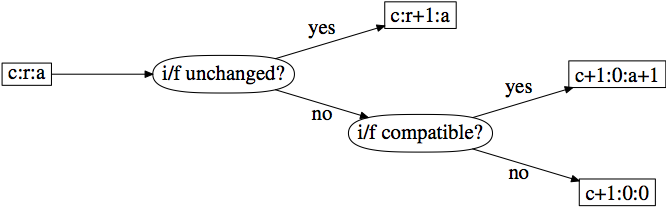
\includegraphics{ssn78-5}
\caption{Updating \code{-version-info} specifications}
\end{figure}

The libtool documentation suggests starting the version-info
specifications at 0:0:0, and this is the default if no
\code{-version-info} option is present.  Since only some Starlink
libraries have this versioning maintained, it is best if you start the
specification at 1:0:0, to distinguish this from those libraries which
have no version-info defined.


You add the \code{-version-info} specification to the libtool command
using the library's \code{LDFLAGS} variable, as follows.  First the
\code{Makefile.am} (from the \code{prm} component): \index{flags,
  compiler and linker}
\begin{terminalv}
libprm_la_SOURCES = \
    $(F_ROUTINES)
    $(PUBLIC_INCLUDES) \
    $(PRIVATE_INCLUDES) \
    PRM_PAR
libprm_la_LDFLAGS = -version-info $(libprm_la_version_info)

libprm_a_la_SOURCES = \
    $(PLATFORM_C)
libprm_a_la_LDFLAGS = -version-info $(libprm_a_la_version_info)
[...]
\end{terminalv}
and then the corresponding section from \code{configure.ac}:
\begin{terminalv}
AC_INIT(prm, 1.3-1, starlink@jiscmail.ac.uk)
# Version-info specifications.  See SSN/78 for guidelines, and update the table
# below for ANY change of version number.
#
# Release    libprm.la      libprm_a.la
#  1.3-1       1:0:0          1:0:0
AC_SUBST(libprm_la_version_info,   1:0:0)
AC_SUBST(libprm_a_la_version_info, 1:0:0)

[...]
\end{terminalv}
There is no automake magic to the \code{libprm\_la\_version\_info}
variable name -- it is just mnemonic, and you are free to change it if
you have a good reason to do so.  Since there is no fixed relationship
between the component version number and the \code{-version-info}
specification, it is important to maintain a simple table of
associations between the two, and the \code{configure.ac} file is a
sensible place to do that.


\section{\label{tool-state}A few remarks on state}
\index{state}

There is quite a lot of state held within the starconf build tree.
This section contains a few notes on where this state is, and how to
handle it.


Since most of the details here are rather intricate, you might save
time by looking at the list of FAQs on state in \secref{state-faqs}.


\emph{Autotool state}: The most obvious state within the tree is the
existence of the \code{configure} and \code{Makefile.in} files which
are the generated by autoconf and automake.  Files \code{config.h.in}
and \code{aclocal.m4}, are also part of this process, inasmuch as they
are generated by autoreconf: \code{config.h.in}\index{config.h.in} is
based on the declarations within \code{configure.ac};
\code{aclocal.m4}\index{aclocal} is a local cache of m4 macros, drawn
from the starconf, autoconf, automake and libtool installations.
Other objects generated by the autotools are the cache directory
\code{autom4te.cache} and the tool links \code{config.guess},
\code{config.sub}, \code{depcomp}, \code{install-sh},
\code{ltmain.sh}, \code{missing} and \code{stamp-h1}.  All of this can
be happily blown away by hand, and a lot of it is removed by
\texttt{make maintainer-clean}\index{make targets!maintainer-clean},
though this doesn't remove things like \code{config.h.in} which are
required for \code{./configure} to run.  Most of this state is
maintained reliably by the dependencies within \code{Makefile.in} --
for example if you update \code{Makefile.am}, then a simple
\texttt{make} will remake \code{Makefile.in} and regenerate
\code{Makefile} before using the new \code{Makefile} to do the build.
If you have removed this state or suspect that it may be out of date,
then autoreconf will always regenerate it -- it's always safe to rerun
autoreconf.


\emph{Configuration state}: When \code{./configure} runs, its most
obvious effect is to transform the \code{.in} files into their
corresponding configured results.  However at the same time, it
creates a log file in \code{config.log} (which can be handy to examine
if a configure script fails or appears to give wrong answers), a cache
in \code{config.cache}\index{config.cache} if you ran
\code{./configure} with the \code{-C} option, it creates the
directory-specific \code{./libtool} script, and it creates a file
\code{config.status}.  This last file holds most of
\code{./configure}'s state, and can be used to either regenerate a
particular file (\texttt{./config.status Makefile}) or else to update
itself (\texttt{./config.status --recheck} has the effect of rerunning
\code{./configure} with the same options such as \code{--prefix} which
were given to the \code{./configure} script last time).  You won't
often have to run \code{./config.status}\index{config.status}
yourself, but it's reassuring to know what it's doing when the
makefile runs it for you.  It is always regenerated afresh by running
\code{./configure}.


\emph{Build state}: The compiled files are obviously part of the build
state, and can be removed by \texttt{make clean}\index{make
  targets!clean} and regenerated with plain \texttt{make}.  Less
obviously part of this state are the directory
\code{.libs}\index{.libs}, which is libtool's' workspace and holds
different types of objects and libraries, and \code{.deps}, which
holds dependency information gleaned as part of the last build.  Less
obviously still are those (few) \code{.in} files which are configured
as part of the build.  As mentioned in \secref{automakeoverview},
so-called `installation directory variables' should be substituted at
make time rather than build time, with a hand-written makefile rule in
\code{Makefile.am}.


\emph{Starconf state}\index{starconf!state, lack of}: There is
essentially no starconf state, since the starconf system's only role
is to manage the \code{bootstrap} file and provide the extra autoconf
macros (installed in the buildsupport part of the tree when starconf
itself is installed). The \code{starconf.status} file is purely a
cache of starconf variables, and allows you to locate the starconf
installation which was used most recently.  At one time, the
\code{starconf.status} file did hold state, and allowed you to
manipulate it, and was even checked in; this is no longer the case.


\emph{Build tree and installation state}: The last noteworthy state is
that in the build tree as a whole.  The top-level makefile requires
some state in order to manage its bootstrapping `make world' build.
This build is organised by representing the build and link
dependencies between components by makefile dependencies between the
components' installed manifests, which are installed in the
\code{.../manifests}\index{manifests!state} directory alongside, and
at the same time, as the component is installed by the \code{install}
Makefile target.  Thus this is state held \emph{outside of the build
  tree}.  If the `make world'\index{make world} build sees that a
manifest file is up-to-date with respect to the dependencies expressed
in \code{Makefile.dependencies} \index{Makefile.dependencies}, it
makes \emph{no attempt to build it}, even if the component itself has
been updated and itself needs rebuilding and reinstalling.  A slight
wrinkle here is that the `buildsupport' tools -- namely starconf and
the autotools -- are not explicitly listed as being a dependency of
anything, since they are in fact a dependency of everything.  Since
they are rather a special case, these are built within the \ top-level
bootstrap script, and the best way to run that `by hand' is via the
command \texttt{./bootstrap --buildsupport}, noting that the remarks
about dependencies above apply to this process also.  Thus, if you
update a component -- including one of the buildsupport components --
and wish the top-level `make world' build to notice this, the best way
to do this is to first delete that component's manifest file from the
installation tree.  This process might change slightly with starconf
developments (see \secref{developments}).


\emph{CVS state}: This isn't really part of the build system as such,
but this seems a good place to point out, or reassure you, that all
the state for a CVS checkout directory is in the files in the CVS
subdirectory, and that all the repository state for the directory is
in the files in the corresponding directory within the repository.


\section{\label{fortran} \index{Fortran} Preprocessable Fortran}


The Starlink build system includes support for preprocessable Fortran,
in both autoconf and automake.


As described in \secref{gnutools}, the installed version of autoconf
is extended with support for preprocessable Fortran, by adding the two
macros \code{AC\_PROG\_FC} and \code{AC\_PROG\_FPP}.


You should use \code{AC\_PROG\_FC}\index{autoconf!macros!AC_PROG_FC}
in preference to the macro \code{AC\_PROG\_F77} described in the
autoconf manual, since the `FC' support in autoconf is more flexible
and more developed than the `F77' support, and the older macro is
likely to be deprecated in coming autoconf releases.  However a
potential problem with the \code{AC\_PROG\_FC} macro is that it
searches for Fortran 9x compilers before Fortran 77 ones.  Fortran 9x
incorporates all of \emph{strict} Fortran 77 as a subset, but no more,
so if you have used any of the common Fortran extensions (which is
sometimes unavoidable), you might find the Fortran compiler objecting.
In this case, you should use the second optional argument to
\code{AC\_PROG\_FC} to specify Fortran 77 as the required dialect:
\begin{terminalv}
AC_PROG_FC([], 77)
\end{terminalv}
See \secref{macro-ac-prog-fc} for full details.


Unlike C, there is no preprocessor defined as part of the Fortran
standard, and this is inconvenient if you wish to use a Fortran
extension if it is available, but not have the compilation fail if it
is absent.  This most commonly applies to the \code{READONLY} keyword
on the Fortran \code{OPEN} statement.  It is possible to use the C
preprocessor, \emph{cpp}, with Fortran, though not completely
reliably, since the underlying syntaxes of C and Fortran are so
different that \emph{cpp} is capable of emitting invalid Fortran in
some circumstances.


Both the Sun and GNU Fortran compilers can handle cpp-style
preprocessor constructs in a Fortran file, avoiding any separate
preprocessing stage.  Sun have produced a Fortran preprocessor,
\emph{fpp}\index{Fortran!fpp (Sun Fortran preprocessor)}, which is
available at \url{http://www.netlib.org/fortran/}: it's freely
available, but not open-source.  And more often than not we can in
fact fall back on simple \emph{cpp}, as long as we have confined
ourselves to the \code{\#include}, \code{\#define} and \code{\#if...}
constructs.  If it comes to that, such simple preprocessing could be
mostly handled with a simple Perl script.


Starlink autoconf and automake between them add support for
preprocessable Fortran.  Autoconf supplies the
\code{AC\_PROG\_FPP}\index{autoconf!macros!AC_PROG_FPP} macro
described in \secref{macro-ac-prog-fpp}, to investigate what compiler
and preprocessor are available, and automake works with the results of
that test to add appropriate support to the generated
\code{Makefile.in}.


For example, you might have in your \code{configure.ac} file the
lines\index{autoconf!macros!AC_FC_OPEN_SPECIFIERS}
\begin{terminalv}
AC_PROG_FC
AC_PROG_FPP
AC_FC_OPEN_SPECIFIERS(readonly,[access='sequential',recl=1])
\end{terminalv}
and have in your \code{my\_io.F} the lines
\begin{terminalv}
#include <config.h>
      SUBROUTINE MYIO(...)

* blah...

      OPEN ( UNIT = LUCON, FILE = IFCNAM, STATUS = 'OLD',
#ifdef HAVE_FC_OPEN_READONLY
     :       READONLY,
#endif
#ifdef HAVE_FC_OPEN_ACCESSSEQUENTIALRECL1
     :       ACCESS='SEQUENTIAL',RECL=1,
#endif
     :       FORM = 'UNFORMATTED', IOSTAT = ISTAT )
\end{terminalv}


The file \code{my\_io.F} is listed in the \code{Makefile.am} as one of
the \code{\_SOURCES} of whatever library or application it contributes
to, alongside the other Fortran files.  If the compiler discovered by
the \code{./configure} script can support preprocessor statements
itself, then the \code{.F} file is treated like any other; if not, and
a separate preprocessing stage is required, then the Makefile handles
this itself.


Note that we are using \code{.F} here as the file extension for
preprocessable Fortran: see \secref{macro-ac-prog-fpp} for discussion.


In those cases where you wish the preprocessing step alone, such as
when you are generating an include file from a template, you
should name the input file with a \code{.F} extension
also.  You will need to include a preprocessing rule in the makefile.
The following idiom might be helpful:
\begin{terminalv}
# Run a .F file through the fpp preprocessor, to produce a file with
# no extension.
# The following deals with case-insensitive filesystems, on which
# foo.f and foo.F would be the same file.  FPP_OUTPUT is
# either "" (in which case the preprocessor writes to foo.f, and
# the filesystem is presumably case-sensitive) or ">$@".
foo: foo.F
        rm -f foo
        $(FPP) $(DEFS) $(DEFAULT_INCLUDES) $(INCLUDES) \
           $(FPPFLAGS) $(CPPFLAGS) foo.F $(FPP_OUTPUT)
        test -f foo || mv foo.f foo
\end{terminalv}
or the following, for a suffix rule
\begin{terminalv}
SUFFIXES = .F
.F:
        rm -f $@
        $(FPP) $(DEFAULT_INCLUDES) $(FPPFLAGS) $(CPPFLAGS) $< $(FPP_OUTPUT)
        test -f $@ || mv $(<:.F=.f) $@
 \end{terminalv}
In this second example, in which we have elided the useful comment,
we have declared the \code{.F} suffix (we wouldn't have to do
this if there were `real' \code{.F} sources in this directory),
and are using the \code{\$<} and \code{\${@}} magic
variables.


In second example, we elided most of the flag variables we included
in the first one, since we probably don't need them.  In case of
doubt, copy the \code{.F.f:} rule in one of the generated
\code{Makefile.in} files.


There is a more elaborate example of this in the
\code{prm} component.


\section{\label{starlink-cvs} Using the Starlink CVS repository}


The Starlink source code is held in a CVS repository, which has public
readonly access.


If you have an account on the repository machine, you have read and
write access to the full source set.  When you are making a fresh
checkout, or giving other commands not within the context of a local
check-out, you should refer to it as
\begin{terminalv}
% cvs -d :ext:\emph{username}@cvs.starlink.ac.uk:/cvs <cvs-command>
\end{terminalv}
where \emph{username} is your username on that
system\index{CVS!repository}; you will need to set the environment
variable \code{CVS\_RSH} to \code{ssh} to connect to the repository.


There is also anonymous CVS access to the repository.  Use
\begin{terminalv}
% cvs -d :pserver:anonymous@cvs.starlink.ac.uk:/cvs login
# password starlink
% cvs -d :pserver:anonymous@cvs.starlink.ac.uk:/cvs <cvs-command>
\end{terminalv}
There is also anonymous web-based access to the repository at
\url{http://cvsweb.starlink.ac.uk}.  See
\url{http://dev.starlink.ac.uk/} for news.


There are a few more details about CVS, including a link to a CVS
Primer, in \secref{tool-cvs}.


Part of the point of the Starlink CVS repository is to give users
ready access to the fully up-to-date sources so that more
sophisticated users can build the most recent application versions for
themselves and even, if they find a bug, offer fixes.  Anyone who
finds a bug is invited to report it through the Project's
bug-reporting system at \url{http://dev.starlink.ac.uk/bugzilla/}, but
if this report comes with fixes, it will be \emph{particularly}
welcome.


If you do have bugfixes to offer, then you should get in touch with
the `owner' of the component to discuss how to give them to the
project.  You will find the owner of a component by looking at the
file \code{component.xml} in the component's checkout directory; this
should list those who have worked on the component, along with someone
nominated as the component's `owner'.


If you make quite a few fixes, then it might be best to give you
committer access to the repository, by giving you an account on the
repository machine.  Talk to someone from the project about setting
that up.

% <!-- Nothing more specific: force folk to go via the person
% they've been submitting patches to. -->

\section{\label{tool-cvs}\index{CVS} CVS}

There is a compact CVS Primer on the web at
\url{http://purl.org/nxg/note/cvsprimer}, and that includes pointers
to fuller documentation.  This section includes a few tips on using
CVS which go beyond that document, or which are more specific to the
Starlink CVS repository.


\subsection{\label{tool-cvs-tagging} CVS and tagging}


Tagging is very important, as it is through tagging that you create
branches, and mark certain sets of files as a set, so that they can be
recovered as a set in future.  The current tagging policy is at
\url{http://wiki.starlink.ac.uk/twiki/bin/view/Starlink/CvsTagging}.


You make a tag with the \texttt{cvs tag} command, while you are in a
directory with a part of the repository checked out:
\begin{terminalv}
cvs tag <tag-name>
\end{terminalv}
This applies the tag to the repository versions indicated by the files
in the current directory.  In the most common case, you have just
finished preparing the set of files for a release, so all the files in
the directory are as you want them to be, and committed.  There's a
slight trap here: if there are any files which are \emph{not}
committed, then it is the repository version which corresponds to the
modified file which is tagged, not the modified file itself (this is
never useful; it is simply a warning to use the \code{tag} command
only in a fully-committed directory).  If you tag a set of files which
are on a branch, then it is (probably unsurprisingly) the branched
files which are tagged.


There is also a \texttt{cvs rtag} command which is similar, but
operates only on the repository.  You won't need to use \code{rtag};
don't confuse the two.


\subsection{CVS and recursion -- checking out only a subtree}
\label{tool-cvs-recursion}
\index{CVS!and recursion}

There are two traps in the way that CVS recurses into subdirectories.
The first is that if a subdirectory is present in the repository but
not in your checkout (most commonly because it has been recently added
to the repository by someone else), then CVS will not by default add
that subdirectory when you do an update, and will give no indication
that it is there.  It is not clear to me why this is a sensible
default, but it is the case nonetheless.  Only if the \code{-d} option
is present on the \texttt{cvs update} command will the `missing'
directory appear.


The other `trap' is that CVS does recurse by default when you do a
checkout.  This is almost always the right thing, but it can be
inconvenient when you want just the top level of the repository.  If
you wanted to check out only the top level, or only the buildsupport
tools, then the command \texttt{cvs -d ???  checkout .} would not be
the right thing, since it would check out the top level and everything
underneath it.  A better set of commands would be
\begin{terminalv}
cvs -d username@cvs.starlink.ac.uk:/cvs co -l .
cvs -d username@cvs.starlink.ac.uk:/cvs co buildsupport
cvs -d username@cvs.starlink.ac.uk:/cvs co thirdparty/fsf
\end{terminalv}
The first line checks out the top level directory but, because of the
\code{-l} (`local') flag, does \emph{not} recurse and check out the
complete repository.  The following lines check out particular
directories, usefully recursing into their children.


If you want to check out just the \code{applications} directory, but
none of its children, use
\begin{terminalv}
cvs -d username@cvs.starlink.ac.uk:/cvs co -l applications
\end{terminalv}
while in the top-level directory.  Don't do \texttt{... co -l .} in
the \code{applications} directory -- you'll get the top-level
directory again.


\chapter{\label{building}Building applications and libraries}

This section applies \emph{only} to building code which has been
checked out of the CVS repository.  It does \emph{not} apply to
building a distribution tarball: that process is nothing more than the
usual:
\begin{terminalv}
% ./configure
% make
% make install
\end{terminalv}
with the usual options for the \code{./configure} script, of which the
most important is \code{--prefix} to control the installation location
of the code.  The default location is typically \code{/star}, though a
particular distribution might have a different value (see
\texttt{./configure --help} for more details).


Recall that the \texttt{make install}, above, installs a manifest
listing the files actually installed, in the directory
\code{/star/manifests} (depending on the value of \code{--prefix},
which defaults to the value shown by \texttt{./starconf.status --show
  STARCONF\_DEFAULT\_PREFIX}).


Most users of this document will likely be concerned only with the
details of building a particular component, and thus concerned
primarily with \secref{buildingcomponents}.


Only rather few users are concerned with building the entire tree, for
example for the nightly build: this is dealt with in
\secref{bootstrapping}.


\textbf{Note}: In all cases, you should \emph{not} have the
\code{INSTALL} environment variable defined.  In old-style Starlink
makefiles this indicated the install location; in the new-style build
system, this location is indicated by the `prefix' described above abd
elsewhere, and the generated Makefiles take the \code{INSTALL}
variable to be the name of a program to use to perform the actual
installation.


\section{\label{top-level-makefile} The top-level Makefile}

The important targets in the top-level makefile are:
\begin{description}

\item[\code{make world}\index{make world}] This target builds the
  whole tree, in an order which respects the dependencies between
  components.  It builds all the targets listed in the variable
  \code{ALL\_TARGETS} within the top-level \code{Makefile.in}.  Those
  targets are install manifests, in the default manifest directory
  (\code{/local/star/manifests} in the example below), so that
  \texttt{make world} both builds and installs the entire software
  set.

  The bootstrap that this is part of is described in more detail in
  \myhref{bootstrapping}{the next section}.

\item[\code{make <manifest-file>}\index{manifests}] As an alternative
  to \texttt{make world}, you may specify a single manifest file.
  This builds and installs the corresponding component, and all of its
  dependencies.  Note that this does nothing if the given manifest
  file is up-to-date with respect to its dependencies on other
  manifest files.  If you have just updated a component, then you can
  rebuild and reinstall it by deleting the component's manifest file
  and remaking it.

\item[\code{make} or \code{make all} \index{make targets!top-level}]
  This recurses into each of the directories listed in
  \code{AC\_CONFIG\_SUBDIRS} within the top-level \code{configure.ac},
  and invokes \texttt{make all} there.  This target brings the tree
  up-to-date after a CVS update, but it does so without respecting the
  dependencies between components.  This target is present for the
  sake of consistency, and as a convenience for bringing the local
  tree up-to-date after a CVS update, and you should not use it as a
  shorthand or alternative for \texttt{make world} above.

\item[\code{make clean}] The targets \code{clean}, \code{distclean}
  and \code{maintainer-clean} simply recurse into the children and
  invoke the corresponding target there.

\item[\code{make install}] This targets does nothing, and is also
  present largely for the sake of consistency.  Depending on the
  context, you should use \texttt{make world} or, if you have just
  updated and rebuild a particular component, then either delete and
  remake its manifest file (as mentioned above), or go to the
  component's directory and use \texttt{make install}.

\end{description}

Note that the building above presumes that all the required code is
checked out of the repository -- it does not handle the checkouts for
you, and if you do not have a required component checked out, it will
simply fail.

\section{Bootstrapping and building the entire tree}
\label{bootstrapping}\index{bootstrapping}

If you wish to build the entire tree after a fresh checkout, you do so
at the top level, using the \code{./bootstrap} script and
\code{Makefile.in} located there.  Neither of these is a `standard'
one, as installed by \emph{starconf} or Starlink automake.


These instructions are echoed in the file \code{README} in the
top-level directory.


The complete procedure for a full build is as shown below, for an
installation into the notional directory \code{/local/star};
explanations follow.
\begin{terminalv}
1% cvs -d :ext:username@cvs.starlink.ac.uk:/cvs checkout .
2% unset STARLINK INSTALL
3% export STARCONF_DEFAULT_STARLINK=/local/star
4% export STARCONF_DEFAULT_PREFIX=/local/star
5% rm -Rf /local/star
6% PATH=/local/star/bin:/local/star/buildsupport/bin:...??? # see note
7% ./bootstrap
... a few harmless warnings, and miscellaneous other chatter
... takes quite a while
8% make configure-deps
... builds some programs needed before configure
9% ./configure -C
... mucho blah-blah-blah
10% make world
... etc
11% ls /local/star/manifests
adam      automake  ems     hlp      messgen  par       sae   star2html  task
ams       chr       fio     lex      messys   parsecon  sla   starconf
atimer    cnf       hds     libtool  misc     pcs       sock  string
autoconf  dtask     hdspar  mers     msp      psx       sst   subpar
\end{terminalv}


Line 1: check out the entire collection from the repository.  See
\secref{tool-cvs-recursion} for hints on how to be more
discriminating, which may be desirable, since not everything in the
repository is controlled by this bootstrapping build, most notably the
contents of the \code{java} directory.


Lines 2-4: unset the \code{STARLINK} and \code{INSTALL} variables, and
set the two starconf variables as shown\index{environment
  variables!STARCONF_DEFAULT_PREFIX}.  For a whole-tree build, these
two should have the same value, to ensure that the build uses only
tools and libraries which have been built at an earlier point in the
build.  For fuller details of these variables, and more information
about controlling the bootstrapping process, see
\secref{bootstrappingonly}.  This example shows sh-style commands for
manipulating the environment; you will of course use the csh-style
\code{setenv} and \code{unsetenv} if you're using that shell.


Also at this point you should review any other environment variables
that might affect the build.  For example, the variables \code{F77},
\code{FC} and \code{CC} will force the build system to use the
specified compilers.  In particular, the default IRAF installation
sets the \code{F77} variable to be a script which works happily in
most cases, but which will \emph{not} work with libtool, and will
cause the build to fail with opaque error messages about being `unable
to infer tagged configuration'.  Unless you do wish to force certain
compilers to be used, it is probably better to unset these variables
before building the software.  Try \texttt{./configure --help} for a
list of `some influential environment variables', and
\secref{configure-script} for more discussion of this issue.


Line 5: the directory where the components are to be installed can be
empty, and need not exist at the start.  It doesn't matter if this is
not empty in fact, since most of the installation tree is not examined
by the build.  The only exception is \code{/local/star/manifests},
since the files in this directory control what is actually built --
see the notes for line 9.


Line 6: put \code{/local/star/bin} and
\code{/local/star/buildsupport/bin} in the path\index{PATH}.  Make
sure that there are \emph{no} Starlink binary directories elsewhere in
the path: running \texttt{which messgen} (for example) at this point
should find nothing.


Line 7: run the \code{./bootstrap} script.  This configures, builds
and installs the `buildsupport' tools -- the autotools plus the
starconf application -- then recursively runs the bootstrap code in a
selection of the directories beneath this one.  The directories the
bootstrap recurses into, in this directory and its children, are those
listed in a \code{AC\_CONFIG\_SUBDIRS} macro in \code{configure.ac}.
After this, you should be able to do
\begin{terminalv}
% which autoconf
/local/star/buildsupport/bin/autoconf
% autoconf --version
autoconf (GNU Autoconf) 2.59
...
%
\end{terminalv}
to verify that the correct tools have indeed been installed in the
correct place.


Line 8: configure the entire tree (the \code{-C} option indicates that
configure should cache its results, speeding up the process).  This
configures this directory and recurses into the children named in
\code{AC\_CONFIG\_SUBDIRS} in this \code{configure.ac} and those below
it.


If you will need to give \code{./configure} some help to find include
files and libraries, you \emph{might} try setting the \code{CFLAGS} or
\code{LDFLAGS} variables in the environment, in the manner described
in \secref{configure-script}.  Note, however, that this is not a
recommended practice.


Line 9: build the entire tree, using the \texttt{make world} target
described in \secref{top-level-makefile}.  The make builds all the
components in an order which ensures that each component is build
after the components it depends on, as declared in
\myhref{macro-declare-dependencies}{\code{STAR\_DECLARE\_DEPENDENCIES}}
\index{dependencies} invocations in those components'
\code{configure.ac} files.  The set of dependencies can be examined
(if you're interested) in the file \code{componentset.xml}, which is
built up from the various directories' \code{component.xml} files, as
reprocessed into \code{Makefile.dependencies}
\index{Makefile.dependencies}.


Note that the dependencies are expressed as dependencies of
components' \emph{manifest} files on each other, and the top-level
makefile is written so that each component is built with the pair of
commands \code{make; make install}, which builds the component then
installs both it and its manifest.  Thus, if you need to ask for a
particular component, foo, to be built, you can do so from the
top-level directory with \texttt{make /local/star/manifests/foo}.


Line 10: after the make, a manifest is installed for each of the built
components.

\section{Building a single component}
\label{buildingcomponents}  \index{components!building}

In \secref{bootstrapping} we saw how you would bootstrap and build the
entire tree, building each component's dependencies before building
the component itself.


If, on the other hand, you wish to build only one component, because
you wish to install the latest and greatest version of some
application, or because you want to work on the CVS version, then you
can do that without, in principle, building the entire code
collection.


The component directories are organised so that you can build a
component from a CVS checkout by moving to the component's directory
and giving the sequence of commands:
\begin{terminalv}
% ./bootstrap
% ./configure
% make
% make install
\end{terminalv}
Before you can do this, however, you will have to do a little
preparation, and there are two cases.


One of the functions of the \code{./bootstrap} script is to regenerate
the \code{./configure} script if necessary, since it is not checked in
to the repository.  This requires that the Starlink-specific autotools
are in your path, and so you must first install these `buildsupport'
tools if they are not installed
already\index{bootstrapping!buildsupport}.  Instructions for that are
\myhref{bootstrappingonly}{below}


There are two cases next.  The first is where you currently have a
built and installed Starlink system which you either built yourself
earlier, or which you installed from a Starlink distribution (note: a
Starlink CD distribution dating before 2005 doesn't count here --
though the applications and libraries are essentially the same, the
distribution and building arrangements changed radically).  The second
case is where you are only interested in one component, but are
starting from scratch, without a pre-existing distribution (of course,
once you successfully complete the second case, you are in the
situation where the first case applies).


\textbf{Case 1 -- pre-built Starlink system:} This is the easy one.
You need check out only the component of interest (see
\secref{tool-cvs-recursion} for notes on that).
\begin{itemize}
\item Change to the component's directory.

\item Define the environment variable
  \code{STARCONF\_DEFAULT\_STARLINK} to point to the top of the
  existing tree, which might be \code{/star} or its equivalent.

\item Define \code{STARCONF\_DEFAULT\_PREFIX} to point to the same
  place if you want to install your new versions there, or to a
  different location if you want to install them separately.

\end{itemize}
At this point you can run \code{./bootstrap} as above, and have these
locations baked in to the configuration as the defaults.


Alternatively, you can control these two locations at configure time,
\emph{after} you have run \code{./bootstrap}.  You control the
installation location with the \code{--prefix} option and the location
of the Starlink tree either with the \code{STARLINK} environment
variable or, better, with the \code{--with-starlink} option.  Although
the use of the \code{STARLINK} variable is supported, it involves less
(easily forgettable) defaulting if you use the \code{--with-starlink}
option instead.  See \secref{configure-script} for details.  Having
said this, setting the \code{STARCONF\_DEFAULT...} variables is
probably preferable, since you don't then have to remember to supply
the options if you run \code{./configure} again.


\textbf{Case 2 -- building from scratch:} This isn't actually much
more complicated, but does take a little longer.  You need to check
out all of the components that your component depends on; since there
is (currently) no automatic way to discover what this set of
components is, in practice you might as well check out the whole
repository.  Since you don't have a pre-built Starlink directory
available, then you will have to build all or most of the tree, before
the component you're interested in can be built.  In this case, follow
the instructions in \secref{bootstrapping} -- which include setting
the \code{STARCONF\_DEFAULT\_...} variables to suitable values -- but
instead of finishing with \texttt{make world} in step 9, do
\texttt{make /mystar/manifests/cpt}, where \code{/mystar} is the
location you have chosen for the installation tree (as specified in
\code{STARCONF\_DEFAULT\_STARLINK}), and \code{cpt} is the component
you are interested in.  This will build and install in turn each of
your component's dependencies, and then the component itself.


If you are doing this because you want the latest and greatest version
of a particular component, then you are finished.


If you are doing this because you want to do development work on the
component, then you might well want to keep the functioning version
separate from your development version.  In this case, you need to go
through this procedure once with \code{STARCONF\_DEFAULT\_STARLINK}
and \code{...\_PREFIX} having the same values, as above.  Next, you
change to the component's directory, and either bootstrap your
development component a second time, with
\code{STARCONF\_DEFAULT\_PREFIX} set to a separate installation
location (you are now in the situation where case 1 applies, above,
and you can give the comments \texttt{./bootstrap; ./configure;
  make}); or else re-run \code{./configure} with its \code{--prefix}
option set to point to that alternative location (the first mechanism
simply sets the default for the second, and is probably preferable for
the reasons mentioned above).


Note that part of the function of the \code{./configure} script is to
find the location of important files and freeze them in to the
Makefile.  Thus the \code{STARLINK} variable is ignored after
configure-time, so that you cannot, in general, change the
\code{STARLINK} variable or change your path, and have new binaries
picked up.


\section{\label{monoliths}\index{monoliths}Building monoliths}


As illustrated in \secref{automakeoverview}, you can build monoliths
in an analogous way to the way you build programs, by declaring the
monoliths as the value of the \code{bin\_MONOLITHS} variable.


Along with the \code{bin\_MONOLITHS} variable, a Makefile must also
declare a set of tasks using the \code{TASKS}\index{monoliths!and
  tasks} primary, and this set will be empty if the monolith is an
ATASK.  If a monolith \code{foo} has a set of tasks \code{a} and
\code{b}, then this declaration will look like this:
\begin{terminalv}
bin_MONOLITHS = foo
foo_TASKS = a b
\end{terminalv}
That is, the tasks are listed without any \code{.ifl} extension.


The \code{foo\_TASKS} primary indicates to automake that there will be
\code{.ifl} files in the local directory corresponding to each of the
tasks in the monolith, that these \code{.ifl} files should be
distributed, and that the appropriate extra links should be made, in
the binary directory, when the monolith is installed\index{symbolic
  links!to monoliths}.  The tasks variable might also be used in the
\code{foo\_SOURCES} variable to declare the dependence of the monolith
on the Fortran files corresponding to the tasks (it would be possible
to automake to have inferred this last step, but it seems clearer
overall to have this dependency at least made explicit).  Automake
permits the usual Makefile variable rewritings, so that if you have a
Fortran file corresponding to each task, then this set is
\verb+$(foo_TASKS:=.f)+which might be useful.


The generated \code{Makefile.in} will install each of the task
\code{.ifc} files, plus the monolith \code{.ifc} file.  The monolith
\code{.ifl} file is constructed by appending each of the task
\code{.ifl} files, wrapped in \code{begin monolith} and
\code{end monolith}, and this generated \code{.ifl} file should not be
included in the repository or the distribution.


If you are building an ATASK\index{ATASKs}, then the task is the same
name as the program.  Indicate this by \emph{omitting} the
\code{...\_TASKS} variable:
\begin{terminalv}
bin_MONOLITHS = foo
# no variable foo_TASKS, since foo is an ATASK
\end{terminalv}
(the extra comment is useful to help document the slightly non-obvious
construction here).  In this case, the only \code{.ifl} file is that
for the ATASK.  The makefile makes sure that this \code{.ifl} file is
distributed, so the file should either exist, or have a rule in the
\code{Makefile.am}.


The \code{MONOLITH} primary allows the prefixes \code{bin},
\code{check} and \code{noinst}, rather like \code{PROGRAMS}.

In order to use the monolith support, you must request this by
including the declaration \code{STAR\_MONOLITHS} in the
\code{configure.ac} file, most rationally near the
\code{AC\_PROG\_CC}-style declarations.


\section{\label{bootstrappingonly}\index{bootstrapping!buildsupport}
  Bootstrapping without building: configuring starconf and the autotools}

If you intend to work only on a single component, then you can
configure and build it as described in \myhref{buildingcomponents}{the
  previous section}.  As described there, the bootstrapping procedure
requires that the `buildsupport' tools -- \emph{starconf} plus
Starlink-specific autotools -- be installed and in your path.


You \emph{must} install the autotools which are part of the CVS
repository, since these have been extended and customised specially
for the Starlink build tree (for the details of the differences, see
\secref{gnutools}).  The standard autotools will not work.


The way to do this is to make sure you have the required components
checked out (see \secref{tool-cvs-recursion}), then go to the top of
the tree and give the command
\begin{terminalv}
% ./bootstrap --buildsupport
\end{terminalv}
This builds and installs the `buildsupport' tools -- namely the
autotools plus starconf -- but does not go on to bootstrap the rest of
the tree.  The functions of the variables
\code{STARCONF\_DEFAULT\_PREFIX} and
\code{STARCONF\_DEFAULT\_STARLINK} were described in
\secref{starconf}: in order to configure starconf at this stage, you
must define these two variables \emph{as environment variables} before
running the \code{./bootstrap} script.  This will cause the tools to
be installed in the directory
\code{\$STARCONF\_DEFAULT\_PREFIX/buildsupport/bin}, and the
configured starconf to configure components, when it is itself
invoked, so that the default value of \code{STARCONF\_DEFAULT\_PREFIX}
is the value given here, as described in the previous section.


You must use this method of configuring starconf and the three
autotools -- autoconf, automake and libtool.


After that, you should put the \code{.../buildsupport/bin} directory
in your path, and start work.


See also \secref{starconf-default-variables} for how to make a version
of the buildsupport tools which has a default installation prefix
different from the buildsupport installation location.


\chapter{Incorporating a package into the Starlink build system}
\label{autoconfing}

The process of adding a package to the build system, and autoconfing
it, is reasonably mechanical.  The main differences from the
traditional build system are as follows.


There is now no \code{./mk} file, and so no platform configuration
using the \code{\$SYSTEM} environment variable.  Instead, all platform
dependencies should be discovered by the configuration process.  It is
only in rather extreme cases that you will need to resort to
platform-specific code, and that should be handled by the starconf
macro \myhref{macro-platform-sources}{\code{STAR\_PLATFORM\_SOURCES}}.


You should try to avoid mentioning or referring to any specific
platform when configuring.  Test for \emph{features}, working with
those you find, and working around those you don't; don't test for
platforms and believe you can reliably then deduce what features are
available.


Traditional Starlink makefiles had two phases, `build' and `install'
(plus the various export targets).  These makefiles often did
on-the-fly editing of scripts as they were being installed, to edit in
version numbers, or the correct path to Perl, for example.  There was
also implicit configuration done in the \code{./mk} script, which
specified platform-specific compiler flags, or versions of `tar'.


GNU-style projects, on the other hand, have three phases, `configure',
`build' and `install', and source file editing happens only in the
first two -- installation consists only of the installation of static
files.  Most configuration editing happens at configure time, when
\code{.in} files are substituted with static information, such as the
absolute paths to programs, determined as part of configuration.  In
the case where the substitution involves installation directory
variables, GNU (and thus general) conventions demand that this be done
at build time, since these directories involve the \code{\$(prefix)}
makefile variable, and it is deemed legitimate for the user to specify
a different value at build time (\texttt{make prefix=xxx}) from that
specified or implied at configuration time.  The user may then specify
a different prefix again at install time (\texttt{make prefix=yyy
  install}) for the purposes of relocating or staging the install, but
this must not invalidate the value of \code{\$(prefix)} which may have
been compiled into applications.  This is discussed in some detail in
section
\href{http://www.gnu.org/software/autoconf/manual/autoconf-2.57/html_node/autoconf_24.html}{4.7.2
  Installation Directory Variables} of the autoconf manual, but you
generally do not have to worry about it, since it is rather rare in
practice that you have to compile installation directories into the
applications and libraries that you build.


In general, whereas traditional Starlink makefiles quite often
performed spectacular gymnastics at install time, GNU-style makefiles
generally do nothing at install time, other than occasionally adding
extra material to the install via one of the installation hooks
supplied by automake (see section
\href{http://www.gnu.org/software/automake/manual/html_node/Install.html}{What
  gets installed} of the automake manual).


In the traditional build system, the master source was regarded as
rather private to the developer who `owned' the code, who was free to
use whatever occult means they desired to produce the sources which
were put into the three distribution objects, `export\_source' (just
the source), `export\_run' (just the executable) and `export' (both).
Now, everything should be put into the CVS repository, including any
code-generation tools either as separate packages or as local scripts,
and it is this source set which is used for nightly builds and the
like.  If you need tools to generate some of the distributed sources,
and they cannot be included in the package for some reason, they
should be checked in, and your component should declare a `sourceset'
dependency on the required tool (see
\secref{macro-declare-dependencies}).


With these remarks out of the way, the following is a description of
the steps involved in bringing first an application into the new fold,
and then a third-party component.


\section{\label{autoconfingexample} Autoconfing a library}


The example here shows the autoconfing of the adam library, chosen
simply because it's relatively simple.


Make a directory to hold the package, and add it to the repository
\begin{terminalv}
% pwd
<cvs-checkout>/libraries/pcs
% mkdir adam
% cvs add adam
Directory /cvs/libraries/pcs/adam added to the repository
% cd adam
\end{terminalv}


Get the complete set of source files, and check them in to the
repository.  This means unpacking all the files in
\code{adam\_source.tar}, which you can find in
\code{/star/sources/pcs/adam} (as it happens).


In this case, the \code{adam\_source.tar} distribution tarball is a
suitable set of sources.  This is not always true, since some Starlink
distributions -- especially some of the larger libraries and
applications -- do quite elaborate processing of their sources in the
process of creating this `source' tarball; in these cases, you should
attempt to obtain a more fundamental set of sources from the package's
developer (if that is not you).


The ideal source for new code is a CVS or RCS repository.  A CVS
repository is easy to import\index{CVS} -- you just tar it up and
unpack it into the correct place within the Starlink repository.  An
RCS repository is barely harder, with the only difference being that
you have to create the Starlink repository directory structure by
hand, and copy the RCS files into place within it.  The only gotcha
with this route is that you must make sure that the permissions are
correct on the resulting repository: you must make sure that everyone
who should have any access to the repository can read \emph{and write}
each of the directories.


CVS repository access is controlled by groups (at least when the
repository is shared), and so each directory within the repository
\emph{must} have a suitable group ownership, with group-write
permissions; each directory must also have the setgid bit set, so that
any directories created within it inherit its gid.  Make sure you
check this as soon as you put the repository in place, or else
everyone will have problems with the repository.  Within the Starlink
repository in particular, all participants are part of the \code{cvs}
group.  In short, you can set the correct permissions on an imported
directory \code{foo} with the commands
\begin{terminalv}
% find foo -type d | xargs chgrp cvs
% find foo -type d | xargs chmod g+sw
\end{terminalv}
This sets the group-owner of each directory to be \code{cvs}, and sets
the group-write and set-group-id bits in the permissions mask (don't
tinker with file permissions, since these affect the permissions of
the checked out files).  You need not worry about file or directory
ownership, since this always ends up being the last person who
committed a file.  Note: The instructions here are based on
observation of CVS repositories; the actual requirements don't seem to
be formally documented anywhere.


Add \emph{all} of the source files, including files like the \code{mk}
script and the old \code{makefile}, which we are about to remove.  Tag
this initial import with a tag
\emph{<component>}\code{-initial-import}, so that it is possible to
recover this old-style distribution if necessary.  As mentioned above,
it is not always completely clear what constitutes the old-style
source set: so don't do this step mechanically, use your judgement,
and above all avoid losing information.  Note also that some of the
infrastructure libraries were added before we settled on this
particular tagging practice, and so lack such an initial tag.


In this present case, the \code{adam\_source.tar} file includes a
Fortran include file containing error codes, \code{adam\_err}; there
are two problems with this.


Firstly, the filename should be uppercase: the file is generally
specified within the program in uppercase, and it should appear thus
on the filesystem.  The traditional makefile works around this by
creating a link from \code{adam\_err} to \code{ADAM\_ERR}, but this
won't work (and indeed will fail messily) on a case-insensitive
filesystem like HFS+, used on OS X.


The second problem is that this is a generated file, though the source
is not distributed, is probably misplaced, and in any case the
generation was probably done on a VAX a decade ago.  All is not lost,
however.  The functionality of the VAX `message' utility is duplicated
in the application \emph{messgen}, in a component of the same name,
along with an application \emph{cremsg} which constructs a source file
from this message file.  Thus it is neither \code{adam\_err} nor
\code{ADAM\_ERR} which we should check in, but the source file
\code{adam\_err.msg} which we reconstruct using \emph{cremsg}.  Thus
with error files, it is the (probably reconstructed) \code{.msg} file
which should be checked in to the repository, and \emph{not} the
\code{\_err}, \code{\_err.h} or \code{fac\_xxx\_err} files which you
may have found in the old-style distribution.


The file \code{adam\_defns} is similar, but this is genuinely a source
file, so we need do nothing more elaborate than rename it to
\code{ADAM\_DEFNS}, then add it to the repository and remove the
original lowercased version.  Many packages have one or two
\code{xxx\_par} files, and these should be similarly renamed to
\code{XXX\_PAR}.
\begin{terminalv}
% tar xf /star/sources/pcs/adam/adam_source.tar
% chmod +x adam_link_adam
% cremsg adam_err
% cvs add *.f mk makefile adam_link_adam adam_defns.h adam_defns adam_err.msg
...
cvs server: scheduling file `adam_err.msg' for addition
cvs server: use 'cvs commit' to add these files permanently
% cvs commit -m "Initial import"
% cvs tag adam-initial-import
% mv adam_defns ADAM_DEFNS
% cvs remove adam_defns
% cvs add ADAM_DEFNS
% rm mk makefile
% cvs remove mk makefile
\end{terminalv}



Note that CVS\index{CVS!and file modes} preserves access modes when it
stores files, so we should make sure that the script
\code{adam\_link\_adam} is executable \emph{before} checking it in,
and we need not bother to make it executable as part of the build
process.  On the other hand, scripts which are substituted by
configure do need to be made executable explicitly, which you do by a
variant of the \code{AC\_CONFIG\_FILES} macro.  The macro invocation
\begin{terminalv}
AC_CONFIG_FILES(foo, [chmod +x foo])
\end{terminalv}
substitutes \code{foo} from source file \code{foo.in} and then makes
it executable.  Note that the sequence
\begin{terminalv}
AC_CONFIG_FILES(foo)
chmod +x foo
\end{terminalv}
would \emph{not} work, since this is one of the cases where autoconf
macros do not simply expand inline to shell code.  For further
discussion, see the section
\href{http://www.gnu.org/software/autoconf/manual/autoconf-2.57/html_node/autoconf_20.html}{Performing
  Configuration Actions} in the autoconf manual.


Create files \code{configure.ac}, \code{Makefile.am} and
\code{component.xml.in} by copying the templates in the starconf
buildsupport directory (\texttt{starconf --show buildsupportdata});
the fields in the \code{component.xml.in} file are discussed in
\secref{componentxml}.  If you have an editor that can use it, you
might also want to create a link to the DTD used for the
\code{component.xml} file, which is in the same directory.  Edit these
files as appropriate, using information in the original Starlink
makefile for guidance (so it's useful to keep a copy of the original
\code{makefile} handy, rather than simply deleting it as illustrated
above).  Then check the files in.


What edits should you make?


The adam \code{Makefile.am} file looks as follows:
\begin{terminalv}
bin_SCRIPTS = adam_link_adam
lib_LTLIBRARIES = libadam_adam.la
libadam_adam_la_SOURCES = $(PUBLIC_INCLUDES) $(F_ROUTINES)
include_HEADERS = $(PUBLIC_INCLUDES)
PUBLIC_INCLUDES = ADAM_ERR ADAM_DEFNS adam_defns.h
F_ROUTINES = \
        adm_acknow.f adm_getreply.f adm_getreplyt.f adm_path.f \
        adm_prcnam.f adm_receive.f adm_reply.f adm_send.f \
        adm_sendonly.f adm_sendt.f adm_trigger.f
\end{terminalv}
Four out of six of these variable declarations are variables
meaningful to automake (see \secref{automakeoverview}), and the other
two are simply copied from the original \code{makefile}.


The adam \code{configure.ac} looks like this:
\begin{terminalv}
AC_INIT(adam, 3.0, starlink@jiscmail.ac.uk)
AC_PREREQ(2.50)
AM_INIT_AUTOMAKE(1.8.2-starlink)
AC_CONFIG_SRCDIR([ADAM_DEFNS])
STAR_DEFAULTS

AC_PROG_FC
AC_PROG_LIBTOOL
STAR_CNF_COMPATIBLE_SYMBOLS

STAR_DECLARE_DEPENDENCIES(build, [sae messys])
STAR_DECLARE_DEPENDENCIES(link,  [chr psx ems messys])

dnl    There is no .msg file in this directory.  The ADAM_ERR file 
dnl    contains only a single definition, of the parameter ADAM__OK.

AC_CONFIG_FILES(Makefile component.xml)
AC_OUTPUT
\end{terminalv}
\index{CNF}\index{dependencies} The first five lines are
straightforward boilerplate (see \secref{autoconfoverview}).  The next
three find a Fortran compiler, declare that we want to use libtool to
build our libraries, and finally that we wish the symbols in that
library to be of the sort that the CNF package is able to handle (see
\secref{macro-cnf-compatible-symbols}).  The `FC' autoconf macros will
search for a Fortran compiler by looking for a f95 compiler before
looking for a f77 compiler; if you know or discover this is
inappropriate, then you can constrain the Fortran dialect that
\code{AC\_PROG\_FC}\index{autoconf!macros!AC_PROG_FC} will look for by
giving a value for its optional dialect argument.  Macro
\code{AC\_PROG\_FC} is not yet documented in the autoconf manual, but
see \secref{gnutools}.


After that, we declare the dependencies.  The dependencies you work
out by any and all means you can.  For a library, the set of `build'
dependencies is determined by the set of components which supply files
which the code here includes.  Grepping for all the Fortran
\code{INCLUDE} statements and all the C \code{\#include} directives is
a good start.  For link dependencies, grepping for \code{CALL} lines
is useful for Fortran, and grepping for
\begin{terminalv}
= *\([A-Za-z][A-Za-z]*__*[A-Za-z][A-Za-z]*\) *(.*
\end{terminalv}
will probably be handy.  In fact, the script
\begin{terminalv}
#! /bin/sh -
sed -n \
        -e 's/^ *\(INCLUDE\|include\) *'\(.*\)'.*/_ \2/p' \
        -e 's/^ *\(CALL\|call\) *\([A-Za-z]*_[A-Za-z]*\).*/\2/p' \
        -e 's/.*= *\([A-Za-z][A-Za-z]*__*[A-Za-z][A-Za-z]*\) *(.*/\1/p' \
        ${1+"$@"} | \
    sort | \
    uniq
\end{terminalv}
should give you the raw material for most of the dependencies you
need.  It doesn't really matter too much if you get this wrong -- you
might cause something to be built slightly later than it might be in
the top-level bootstrap, might cause some eventual user to have to
download one package more than they have to, or might create a
circular dependency and break the nightly build, in which case you'll
find out soon enough.


See \secref{macro-declare-dependencies} for the description of the
various types of dependencies you can specify here.


By the way, remember (because everyone forgets) that there are no
components \code{err} and \code{msg}: all of the \code{err\_} and
\code{msg\_} functions are in the \code{mers} component.


The next couple of lines tells you that we lied outrageously, above,
when we were talking about \code{.msg} files.  Though the remarks
there are true enough in general, the \code{ADAM\_ERR} file is
special, and doesn't come from any \code{.msg} file.  This is
surprising enough that it's worth making a remark to this effect in
the \code{configure.ac} file.


Finally, we list the files that should be configured.  Essentially all
starconf-style configure files should have at least these two files
mentioned here.


Now run starconf.  As described in \secref{starconf}, this adds some
required files, and checks that the directory looks right.  It will
look something like this:
\begin{terminalv}
% starconf
starconf-validate: the following files are required but do not exist:
        bootstrap
starconf-validate: the following files should be checked in, but aren't
        Makefile.am configure.ac bootstrap component.xml.in component.xml
Configuring with STARCONF_DEFAULT_STARLINK=/export3/sun
Configuring with STARCONF_DEFAULT_PREFIX=/export3/sun
Creating bootstrap
\end{terminalv}

That complained that the file bootstrap wasn't present, and then went
on to install one for you; it listed a number of files which should be
checked in; and it added a bootstrap script.  The starconf application
actually does the checking by running the \emph{starconf-validate}
script, which you can run yourself independently if you wish.


Now you have a bootstrap file, so run it:
\begin{terminalv}
% ./bootstrap
starconf-validate: the following files should be checked in, but aren't
        Makefile.am configure.ac bootstrap component.xml.in component.xml
Configuring with STARCONF_DEFAULT_STARLINK=/export3/sun
Configuring with STARCONF_DEFAULT_PREFIX=/export3/sun
File bootstrap already exists, not overwriting
autoreconf --install --symlink
configure.ac: installing `./install-sh'
configure.ac: installing `./missing'
\end{terminalv}
The bootstrap script always re-runs starconf if it can, so this
reminds you that you still haven't checked those files
in\index{starconf-validate}.  It also runs autoreconf
(\secref{autoreconf}) for you, installing the helper files that
requires, and constructing \code{configure} from \code{configure.ac}
and \code{Makefile.in} from \code{configure.ac} and
\code{Makefile.am}.


Now, finally, you can try \code{./configure} and \code{make}.  That
might just work.


Iterate until success.


When the code is working, you will might want to add it to the set of
components which are explicitly built.  To do this, add it to the
\code{ALL\_TARGETS} variable in the top-level \code{Makefile.in}.
Next, go to the parent directory of the directory you have just added:
the \code{configure.ac} file there will almost certainly have a
skeleton \code{configure.ac} which includes a
\code{AC\_CONFIG\_SUBDIRS} line, to which you should add your newly
working directory.


\section{\label{buildsystem-interface} The build system `interface'}


The previous section describes the steps required to bring a component
into the build system.  This section makes reasonably explicit what
was implicit in that previous section, by describing the `interface'
between the build system and a particular component.  The word
`interface' is in scare-quotes there because this interface isn't
formal and isn't enforced, but it should be useful as a check-list and
as an overview.


1. \code{component.xml}: every component has to have an XML-valid
instance of this, as defined by \code{componentinfo.dtd} with element
\code{<component>} at the root level (see \secref{componentxml}).


2. A Makefile which implements most/all of the GNU standard
targets\index{make targets}.  I think we actually use `all' (default),
`install', `check' and `dist' as part of the build system, and I've
mentioned `clean', `distclean', and `maintainer-clean' elsewhere in
this document.  The GNU coding standards add `uninstall',
`install-strip', `mostlyclean', `TAGS', `info', `dvi', none of which
we probably care much about (uninstalling should probably be handled
by whatever package-management tool we settle on, rather than a
makefile).  The build system does \code{cd xxx; make; make install}
for component \code{cpt}, where \code{xxx} is the contents of
\code{/componentset/component[@id='cpt']/path} in the
\code{componentset.xml} file.  This requirement comes for free, given
that you use a \code{Makefile.am} file and automake, and this
requirement is mentioned only for completeness.


3. Doing `make install' additionally installs a
\code{\$prefix/manifests/cpt} manifest, which is a valid instance of
the \code{componentinfo.dtd} DTD with the \code{<manifest>} element at
the root level.  Again, this step comes for free when you use the
automake system.


4. Bootstrapping: the top-level bootstrap script includes a call to
`autoreconf'.  This configures the whole tree, using autoconf's
built-in support for recursing, based around the macro
\code{AC\_CONFIG\_SUBDIRS}, and you should make sure that any new
components are pulled in to this mechanism.  Apart from that, the
behaviour of the \code{./configure} scripts isn't really part of this
`interface', except that components are linked in to the tree-wide
configure by virtue of being mentioned in the \code{configure.ac}
scripts in their parent (see the `bridging' scripts in
\code{applications/configure.ac} and \code{libraries/configure.ac}).
If, for some reason, you wished to incorporate a large number of
components in a new tree (perhaps you want to include some complicated
tree of Perl modules, for example), then you would similarly
hand-write some `bridging' scripts, which preserve the property that
your new tree is configured (doing whatever is required in a
particular situation) when its parent is.




\section{\label{autodistrib}\index{distribution} Distribution of
  components}

The \code{Makefile.in} files which automake generates generally
handles distribution pretty successfully, and the command \texttt{make
  dist} will usually do almost all the work of packing your files into
a distribution which can be built portably.  In some cases, however,
you have to give it a little help.


There are two potential problems.  Firstly, automake may not be able
to accurately work out the set of files which ought to be distributed.
Consider the following makefile fragment (this, along with the other
examples in this section, is from the AST distribution, which presents
a variety of distribution problems):
\begin{terminalv}
noinst_PROGRAMS = astbad
astbad_SOURCES = astbad.c pointset.h
AST_PAR: ast_par.source astbad
    sed -e 's/<AST__BAD>/'`./astbad | tr 'E' 'D'`'/' ast_par.source >$@
\end{terminalv}
Automake packages anything mentioned in a \code{\_SOURCES} variable,
so \code{astbad.c} and \code{pointset.h} are included in the
distribution automatically.  However it does not attempt to work out
every consequence of the makefile rules, and so fails to spot that
\code{ast\_par.source} is going to be needed on the build host.  In
general, a file which is mentioned only in a makefile dependency will
not be automatically distributed by automake.  Files such as this
should be included by the distribution by listing them in the value of
the \code{EXTRA\_DIST}\index{distribution!EXTRA_DIST} variable:
\begin{terminalv}
EXTRA_DIST = ast_par.source
\end{terminalv}


Automake also supports the \code{dist\_} and \code{nodist\_} prefixes
to automake variables\index{distribution!dist prefix}.  These can be
used to adjust automake's defaults for certain primaries.  Automake
does not distribute \code{\_SCRIPTS} by default (this is since they
are sometimes generated, but I for one find this counter-intuitive),
so if you want a script to be distributed, you must use a prefix:
\begin{terminalv}
bin_SCRIPTS = ast_link
dist_bin_SCRIPTS = ast_link_adam
noinst_SCRIPTS = ast_cpp
dist_noinst_SCRIPTS = makeh
\end{terminalv}
\index{installation!noinst prefix} We see all four common
possibilities here: \code{ast\_link\_adam} and \code{makeh} are needed
in the distribution but need no configuration, and so should be
distributed as they stand; \code{ast\_link} and \code{ast\_cpp} are
configured, so these files should not be distributed, since the
corresponding \code{.in} files are (as a result of being mentioned in
\code{AC\_CONFIG\_FILES}).  Also \code{ast\_cpp} and \code{makeh} are
used only to build the library, and are not installed.  You could get
the same effect by listing \code{ast\_link\_adam} and \code{makeh} in
\code{EXTRA\_DIST}, but it is probably a little less opaque if all the
information about particular files is kept in one place.


Incidentally, the other occasionally important `prefix-prefix' like
\code{dist} is \code{nobase}\index{installation!nobase prefix}.  See
\secref{nobase-faq}.


On the other hand, files in \code{\_SOURCES} variables are distributed
by default, so you must turn this off if one of these files is
generated at configure time:
\begin{terminalv}
libast_la_SOURCES = \
    $(GRP_C_ROUTINES) \
    $(GRP_C_INCLUDE_FILES) \
    $(GRP_F_INCLUDE_FILES) \
    ast_err.h
nodist_libast_la_SOURCES = \
    ast.h \
    AST_PAR
\end{terminalv}


Though the set of included files is deterministic, I find it is not
terribly predictable, and the best way to do this sort of tidyup is by
making a distribution, trying to build it, and thus discovering which
files were left out or included by accident.  There is no harm in
listing a file in \code{EXTRA\_DIST} which would be included
automatically.


For fuller detail on automake's distribution calculations, see section
\href{http://www.gnu.org/software/automake/manual/html_node/Dist.html}{What
  Goes in a Distribution} of the automake manual.


The second distribution problem is that some Starlink components do
quite a lot of work at distribution time, building documentation or
generating sources, generally using programs or scripts which are not
reasonably available on the eventual build host.  This is in principle
out of scope for automake and autoconf, but since it is common and
fairly standardised in Starlink applications, Starlink automake and
autoconf provide some support for pre-distribution configuration.


All configuration tests in \code{configure.ac} should be done
unconditionally, even if they are only meaningful prior to a
distribution -- they are redundant afterwards, but cause no problems.
Any files which should be present \emph{only} prior to the
distribution should be listed in \code{configure.ac} inside macro
\myhref{macro-predist-sources}{STAR\_PREDIST\_SOURCES}\index{starconf!macros!STAR_PREDIST_SOURCES}.
The \code{./configure} script expects to find either all of these
files or none of them, and if it finds some other number, it will warn
you.  If it finds these files, it concludes that you are in a
pre-distribution checkout, and sets the substitution variable
\code{@PREDIST@} to be empty; if it finds none, it concludes that you
are in a distributed package, and defines \code{@PREDIST@} to be the
comment character \code{\#}.  This means that makefile fragments which
are only usable prior to distribution should all be prefixed with the
string \code{@PREDIST@}, and they will thus be enabled or disabled as
appropriate.  The distribution rules mentioned above mean that any
configuration of such undistributed files must be done by hand in the
\code{Makefile.am}, and not by \code{AC\_CONFIG\_FILES}, since this
macro automatically distributes the files implied by its arguments.


For example, the AST \code{configure.ac} has:
\begin{terminalv}
STAR_LATEX_DOCUMENTATION([sun210 sun211], [sun210.htx_tar sun211.htx_tar])
STAR_PREDIST_SOURCES(sun_master.tex)
STAR_CHECK_PROGS(star2html)
STAR_CHECK_PROGS(prolat, sst)   # prolat is part of SST
\end{terminalv}
\index{documentation!complicated} The \code{sun\_master.tex} file is
used when the SUN/210 and SUN/211 files are being generated, and
should not be distributed.  Since the process of generating the
documentation uses application \code{star2html}, we check for this and
for \code{prolat} (and thus do this redundantly even after
distribution).  Most components can get away with the one-argument
version of \code{STAR\_LATEX\_DOCUMENTATION} which avoids these
complications, and does the equivalent of the \code{star2html} check
internally.


This AST configure script also has
\begin{terminalv}
STAR_PREDIST_SOURCES(error.h.in version.h.in)
\end{terminalv}
and carefully avoids calling
\code{AC\_CONFIG\_FILES(error.h version.h)}.  It still has to
configure these files prior to distribution, so this has to be done in
the \code{Makefile.am}:
\begin{terminalv}
@PREDIST@predist_subs = sed \
@PREDIST@    -e 's,@star_facilitycode\@,$(star_facilitycode),' \
@PREDIST@    -e 's,@PACKAGE_VERSION\@,$(PACKAGE_VERSION),' \
@PREDIST@    -e 's,@PACKAGE_VERSION_MAJOR\@,$(PACKAGE_VERSION_MAJOR),' \
@PREDIST@    -e 's,@PACKAGE_VERSION_MINOR\@,$(PACKAGE_VERSION_MINOR),' \
@PREDIST@    -e 's,@PACKAGE_VERSION_RELEASE\@,$(PACKAGE_VERSION_RELEASE),' \
@PREDIST@    -e 's,@PERL\@,$(PERL),'
@PREDIST@error.h: error.h.in
@PREDIST@	rm -f $@; $(predist_subs) $< >$@
@PREDIST@version.h: version.h.in
@PREDIST@	rm -f $@; $(predist_subs) $< >$@
\end{terminalv}
(this is the same technique that was illustrated in passing in the
discussion of `installation locations' in \secref{automakeoverview}).
The leading \code{@PREDIST@} strings mean that this stanza causes no
problems after distribution, when the \code{error.h.in} files are not
present.  See \secref{macro-predist-sources} for more details.

This is admittedly a rather crude technique, but it is a lot less
fragile than the more elegant alternatives.


\subsection{\label{rolldistribution} \index{distribution}
Making a distribution}


In general, the details of making distributions are outside the
(current) scope of this document.  However there is one aspect we can
usefully mention, since it interacts with the buildsupport tools which
configure the distribution.


Normally, when you \code{./bootstrap} a directory, it arranges to
install it by default in a location governed by starconf (see
\secref{starconf} for details).  Since this default is a location on
your local machine, it might not be appropriate for a distribution
tarball.  In that case, you will probably want to ensure that the
built distribution will install into \code{/star} (or
\code{/usr/local} perhaps).  There are multiple ways you can do this.


\subsubsection{\label{rolldistribution-tree} A distribution from the complete tree}

If you are doing this for a complete tree, with the intention of
building all the software and rolling distribution tarballs with the
result, then the procedure you should use is as follows.
\begin{enumerate}
\item Check out the repository as usual.


\item Identify the directory you want to be the default installation
  location for the distributed components, and the directory in which
  the distributed tarball will find other tools.  These will typically
  be the same, but if you are distributing a development or updated
  version, you might want the default prefix to be \code{/stardev} but
  the default Starlink directory to remain \code{/star}.  Set these as
  the \code{STARCONF\_*} defaults.
\begin{terminalv}
% export STARCONF_DEFAULT_PREFIX=/star
% export STARCONF_DEFAULT_STARLINK=/star
\end{terminalv}
If this directory really is just \code{/star} then these settings
could in principle be omitted and the variables simply left unset,
since \code{/star} is the default for both, but declaring them
explicitly avoids ambiguity.  The directory mentioned here need not
exist or be writable.


\item Identify a directory tree to hold the products as you build
  them; I'll use \code{/tmp/star} as an example.  Since this directory
  will receive the the buildsupport tools, and other tools built
  during the build, it will need to be included in your PATH.
\begin{terminalv}
% PATH=/tmp/star:$PATH
\end{terminalv}


\item Bootstrap the tree, creating as you do so a set of buildsupport
  tools which are put in this working tree.  If you do not add this
  option then the bootstrap will attempt to install the buildsupport
  tools in \code{/star}.
\begin{terminalv}
% ./bootstrap --buildsupport-prefix=/tmp/star
\end{terminalv}


\item Configure the tree, here overriding the \code{STARCONF\_*}
  defaults.
\begin{terminalv}
% ./configure -C --prefix=/tmp/star --with-starlink=/tmp/star
\end{terminalv}
This will install the components into \code{/tmp/star}, with later
components using tools installed there earlier, but with the
\code{./configure} scripts within those components written so that
they will still install in \code{/star} by default.


\item Then build the tree as usual.
\begin{terminalv}
% make world
\end{terminalv}
The manifests will end up in \code{/tmp/star/manifests}.


\end{enumerate}



After this process has completed, if you go to a built component and
make a tarball using \texttt{make dist}, then this tarball will
install in \code{/star} by default, which you can check using
\texttt{./configure --help}.



\subsubsection{\label{rolldistribution-single} Distributing a single
  component}

If, on the other hand, you wish to create a distribution tarball of a
single component, then you do not have to reconfigure the entire tree
to do so (fortunately).


The more robust way is to create a special set of buildsupport tools
which have the desired directory as their default prefix.  Say you
want the distribution to install by default in \code{/star}, but have
these special buildsupport tools installed in
\code{/local-star/makedist} (for example) .  Do that as follows:
\begin{terminalv}
% STARCONF_DEFAULT_PREFIX=/star ./bootstrap --buildsupport \
    --buildsupport-prefix=/local-star/makedist
\end{terminalv}
(or use \texttt{env ...} on csh-type shells; you would typically
specify \code{STARCONF\_DEFAULT\_STARLINK} here,
too).\index{bootstrapping!buildsupport}.  Setting the two
\code{STARCONF\_*} variables is actually redundant, here, since both
have \code{/star} as their default, but it does no harm and can make
things usefully explicit.


At this point, you can check out the appropriate version of your
software (probably via a CVS export of a particular tag), put this
\code{/local-star/makedist/bin} in your path (rehashing if you are
using csh), and call \texttt{./bootstrap; ./configure; make dist} as
usual.  The command \texttt{./configure --help} will show you the
default prefix for this \code{./configure} script.


An alternative way is to use the
\code{acinclude.m4}\index{acinclude.m4} method described in
\secref{starconf-default-variables}, setting \code{OVERRIDE\_PREFIX}
to \code{/star} (for example).  When you run \code{./bootstrap} after
that, the given prefix will be used instead of the prefix baked into
the installed buildsupport tools.


That is, to create a distribution of component \code{foo}, located in
\code{libraries/foo} in the repository, you should \emph{tag} the
source set with a suitable release tag, such as \code{foo-1-2-3}, and
then, in a temporary directory, do the following:
\begin{terminalv}
% cvs -d \emph{???} export -r foo-1-2-3 libraries/foo
% cd libraries/foo
% echo 'm4_define([OVERRIDE_PREFIX],[/star])' >acinclude.m4
% ./bootstrap
% ./configure
% make dist
\end{terminalv}
This will leave a tarball such as \code{foo-1.2-3.tar.gz} in the
current directory.



\section{\label{regressiontests}\index{tests} Regression tests}

Automake provides some simple support for regression tests.  There is
a (terse) description of these in the automake manual, in the section
\href{http://www.gnu.org/software/automake/manual/html_node/Tests.html}{Support
  for test suites}, but it lacks any example.  You run the tests with
\texttt{make check}, after the build, but before the component is
installed.


        You can set up tests as follows.
\begin{terminalv}
TESTS = test1 test2
check_PROGRAMS = test1 test2

test1_SOURCES = test1.f
test1_LDADD = libemsf.la libems.la `cnf_link`

test2_SOURCES = test2.c
\end{terminalv}


The \code{TESTS} variable lists a set of programs which are run in
turn.  Each should be a program which returns zero on success, and if
all the programs return zero, the test is reported as a success
overall.  If a non-portable test makes no sense on a particular
platform, the program should return the magic value 77; such a program
will not be counted as a failure (so it's actually no different from
`success', and the difference seems rather pointless to me).  A
\code{PROGRAMS} `primary' (see \secref{automakeoverview} for this
term) indicates that these are programs to be built, but the `prefix'
\code{check} indicates that they need be built only at `make check'
time, and are not to be installed.


The \code{SOURCES} primary is as usual, but while the \code{test2}
program is standalone (it's not clear quite how this will test
anything, but let that pass), the \code{test1} program needs to be
linked against two libraries, presumably part of the build.  We
specify these with a \code{LDADD} primary, but note that we specify
the two libraries which are actually under test as two \emph{libtool
  libraries}, with the extension \code{.la}, rather than using the
\code{-lemsf -lems `cnf\_link`} which \code{`ems\_link`} uses as its
starting point (this example comes from the \code{ems} component).
That tells libtool to use the libraries in this directory, rather than
any which have been installed.


The fact that test programs must return non-zero on error is
problematic, since Fortran has no standardised way of controlling the
exit code.  Many Fortran compilers will let you use the \code{exit}
intrinsic:
\begin{terminalv}
rval = 1
call exit(rval)
\end{terminalv}
to return a status.  Since this is test code, it doesn't really matter
that this \emph{might} fail on some platforms, but if this worries
you, then write the test code as a function which returns a non-zero
integer value on error, and wrap it in a dummy C program:
\begin{terminalv}
test1_SOURCES = test1.f test1_wrap.c
test1_wrap.c:
	echo "int main() { exit (test1_()); }" >test1_wrap.c
\end{terminalv}


If the tests you add use components other than those declared or
implied as component dependencies (see
\secref{macro-declare-dependencies}), then you should declare the full
set of test dependencies using
\code{STAR\_DECLARE\_DEPENDENCIES([test], [...])}.


\section{\label{importing-thirdparty} Importing third-party sources}


\textbf{NOTE: this section is subject to a little change.}  The
guidance in this section is to some extent subject to change as we get
more experience including third-party sources into the tree.


If an application needs to rely on a non-Starlink application, and
especially if it relies on a modified version, then the sources for
that application should be checked in to the \code{thirdparty/} part
of the tree.


There are two stages to this.  Firstly we have to import a
distribution version of the software, and secondly we have to bring it
in to the Starlink build system.


The example here is the GNU m4 distribution, which is one of the
buildsupport tools necessary on Solaris, which has a non-GNU m4
(autoconf relies on language extensions in GNU m4, which is therefore
required).  The first step is rather mechanical, the second better
introduced by example.


First, we get and import the sources (see the fuller details in the
\href{http://www.cvshome.org/docs/manual/}{CVS manual}):
          \begin{terminalv}
% cd /tmp
% wget http://ftp.gnu.org/pub/gnu/m4/m4-1.4.tar.gz
% tar xzf m4-1.4.tar.gz
% cd m4-1.4
% cvs -d :ext:username@cvs.starlink.ac.uk:/cvs import \
    -ko -m "Import of GNU m4 1.4" \
    thirdparty/fsf/m4 FSF m4-1-4
\end{terminalv}


The \code{-ko} option turns off any keyword expansion for the
newly-imported files.  Thus they will retain the values they had when
they were imported.  This appears to be the practice recommended by
the CVS manual, though it is not absolutely clear that it is best, and
this should not be taken as a firm recommendation.


The \code{thirdparty/fsf/m4} argument is the location of the new
component within \emph{our} repository, the path to which will be
created for you if necessary.  FSF -- the `Free Software Foundation'
-- is the `vendor' in this case, and this is used for the location
within the \code{thirdparty/} tree as well as the next CVS argument.
CVS uses this vendor argument as the name of the branch this new
import is nominally located on.


Finally, this import command tags the imported files with the tag you
give as the last argument.  This should use the same convention as
other tags within the Starlink repository, namely the component name
and version number.


Note that we import a \emph{distribution tarball} of the source,
namely one including the \code{configure} script and any other
generated files.  This is because we cannot reliably bootstrap the
original sources if they, for example, and also so that we can
reliably track any future releases of the tarball.  Even if the
component has a public CVS archive, resist the temptation to import a
snapshot of that.


Now that the source set is in the repository, you can go back to your
checkout tree and check the new component out:
          \begin{terminalv}
% cd <checkout-tree>
% cvs -d :ext:username@cvs.starlink.ac.uk:/cvs co thirdparty/fsf/m4
[blah...]
% cd thirdparty/fsf/m4
% cvs status -v configure.in
===================================================================
File: configure.in      Status: Up-to-date

   Working revision:    1.1.1.1
   Repository revision: 1.1.1.1 /cvs/thirdparty/fsf/m4/configure.in,v
   Sticky Tag:          (none)
   Sticky Date:         (none)
   Sticky Options:      -ko

   Existing Tags:
        m4-1-4                          (revision: 1.1.1.1)
        FSF                             (branch: 1.1.1)
\end{terminalv}
We see that the newly-imported files have been put on the 1.1.1
branch, named \code{FSF}.  Any files we add to this component, and any
files we modify, will go on the trunk.


What you do next depends on how easy it is to configure the new
component.  We'll look at three examples, the \code{m4} component,
containing the GNU version of m4, the \code{cfitsio} component,
containing the HEASARC FITS library, and the \code{tclsys} component,
containing a distribution of Tcl.
\begin{enumerate}
\item The \code{m4} configuration is quite regular (as befits a core
  GNU component), and so admits of reasonable adaptation in place, by
  simply editing the configuration files included in the distribution
  (and then, despite what we said above, regenerating the distributed
  \code{./configure} script.

\item The \code{cfitsio} distribution comes with its own configure
  scripts, but they are generated using a rather old version of
  autoconf, so we want to avoid touching them.  However the build is
  basically rather simple, and only a few built files need to be
  installed.  This component shows how to wrap a distribution's own
  configuration in a straightforward way.

\item The \code{tclsys} component, on the other hand comes with its
  own fearsomely intricate configuration and installation mechanism,
  which we want to disturb (or indeed know about) as little as
  possible.  This section shows how to wrap such an installation in
  the most general way.

\end{enumerate}



\subsection{ \index{components!m4}Configuring m4}


The first thing to do is to add the \code{component.xml.in} file:
\begin{terminalv}
% cp `starconf --show buildsupportdata`/template-component.xml.in \
      component.xml.in
\end{terminalv}
after which we edit \code{component.xml.in} appropriately.  This
editing turns out to be slightly more intricate than usual: the
\code{configure.in} file is old-fashioned enough that it does not
define the substitution variables that \code{component.xml.in} is
expecting, and it requires a slightly closer inspection of
\code{configure.in} to determine what these should be
(\code{{@}PRODUCT{@}} and \code{@VERSION@} in this case).  Although
this step seems redundant, it is best to have this file configured
rather than completely static, so that the generated
\code{component.xml} will remain correct when and if a new version of
the `m4' component were imported.  Having said that, ensure that the
\code{<bugreports>} element in the \code{component.xml.in} file points
to a Starlink address -- we don't want bugs in \emph{our}
modifications to be reported to the original maintainers.


Note that it is the now-deprecated \code{configure.in} file that is
the autoconf source in this component, and that it has now-deprecated
syntax; there is no need to update this.  When we run autoreconf, we
discover that this is not the only obsolete feature, and we have to do
some futher mild editing of \code{configure.in} before it is
acceptable to the repository version of autoconf, though it still
produces a good number of warnings.  These don't matter for our
present purposes: the \code{./configure} which autoreconf produces
(and which we commit) still works, and the component builds and runs
successfully.  If the \code{configure.in} were old enough that our
current autoconf could not process it at all, then we might consider
retrieving and temporarily installing an older version of autoconf --
the \code{./configure} script includes at the top a note of the
autoconf version which produced it.\index{autoconf!old versions}


In order for the new component to be a good citizen in the Starlink
build tree, it needs to install a file manifest as part of the
\code{install} target\index{manifests!and third-party code}.  Add to
the \code{configure.in} file the lines
\begin{terminalv}
: ${STAR_MANIFEST_DIR='$(prefix)/manifests'}
AC_SUBST(STAR_MANIFEST_DIR)
\end{terminalv}
If we were using Starlink automake, this would be enough to prompt it
to include support for installing a manifest in the \code{Makefile.in}
it generates.  The GNU m4 distribution does not, however, use
automake, so we need to add this by hand.  The following additions to
\code{Makefile.in} do the right thing, though they are rather clumsier
than the support that Starlink automake adds:
\begin{terminalv}
STAR_MANIFEST_DIR = @STAR_MANIFEST_DIR@

[...]

# Change the install target from the default
install: config.h install-manifest.xml
         for subdir in $(SUBDIRS); do \
             echo making $@ in $$subdir; \
             (cd $$subdir && $(MAKE) $(MDEFINES) $@) || exit 1; \
         done
         $(srcdir)/mkinstalldirs $(STAR_MANIFEST_DIR)
         $(INSTALL_DATA) install-manifest.xml $(STAR_MANIFEST_DIR)/$(PRODUCT)

# Add the install-manifest.xml target
install-manifest.xml: all
        rm -Rf STAGING
        mkdir STAGING
        $(MAKE) prefix=`pwd`/STAGING install
        rm -f $@
        echo "<?xml version='1.0'?>"                            >$@
        echo "<!DOCTYPE manifest SYSTEM 'componentinfo.dtd'>"   >>$@
        echo "<manifest component='$(PACKAGE_NAME)'>"           >>$@
        echo "<version>$(PACKAGE_VERSION)</version>"            >>$@
        echo "<files>"                                          >>$@
        find STAGING -type f | sed 's,^.*STAGING,$(prefix),'    >>$@
        echo "</files>"                                         >>$@
        echo "</manifest>"                                      >>$@
        rm -Rf STAGING
\end{terminalv}
(if you look at \code{thirdparty/fsf/m4/Makefile.in} you will see that
we actually need to have \code{PRODUCT} and \code{VERSION} there
instead of the more general \code{PACKAGE\_NAME} and
\code{PACKAGE\_VERSION} above).  Note that the actual installation
happens within the rule for \code{install-manifest.xml} -- this
guarantees that the \code{\$(prefix)} stored in the manifest is the
same as the \code{\$(prefix)} actually used for the installation.


Since we are creating this manifest entirely by hand, we are
responsible for ensuring that the resulting file conforms to the DTD
in \code{componentinfo.dtd} (in the starconf \code{buildsupportdata}
directory).


We add the \code{component.xml.in} file to the repository, and look at
what we have.
\begin{terminalv}
% cvs add component.xml.in
% cvs -n update
\end{terminalv}
This tells us that \code{configure}, \code{configure.in} and
\code{config.h.in} have been modified, and \code{component.xml.in}
added, but we also discover that files \code{stamp-h.in},
\code{doc/stamp-vti} and \code{doc/version.texi} have also been
modified, as part of the regeneration of the \code{./configure}
script.  The modification to the stamp file \code{stamp-h.in} we
should probably commit, to avoid dependency niggles in the future, but
the meaningless changes to the two \code{doc/} files we can just
discard:
\begin{terminalv}
% cvs commit -m "Add component.xml template" component.xml.in
% cvs commit -m "...blah..." configure configure.in config.h.in
% cvs commit -m "Stamp file regenerated by autoreconf" stamp-h.in
% rm doc/stamp-vti doc/version.texi
% cvs update doc
\end{terminalv}


We can see that the changes to \code{configure.in} are now on the
trunk for this component, rather than the FSF branch.
\begin{terminalv}
% cvs status configure.in
===================================================================
File: configure.in      Status: Up-to-date

Working revision:    1.2
Repository revision: 1.2     /cvs/thirdparty/fsf/m4/configure.in,v
Sticky Tag:          (none)
Sticky Date:         (none)
Sticky Options:      -ko
\end{terminalv}

\subsection{Configuring CFITSIO}
\label{config-cfitsio}
\index{components!cfitsio}

The \code{cfitsio} component wraps the HEASARC FITS library of the
same name, and installs from it the library itself, plus a few header
files.  Although we probably could adapt the library's distributed
autoconf script, that script is sufficiently old, and there are
sufficiently few components installed, that it is less trouble to
simply wrap this configuration in another one.


The \code{cfitsio} component contains a \code{cfitsio/} directory
containing the distributed library source.  Along with it are the
usual \code{component.xml.in} file, copied from the template in
\code{`starconf --show buildsupportdata`}, and \code{Makefile.am} and
\code{configure.ac} files, which are too different from the template
ones for them to be helpful.


The \code{configure.ac} looks like this:
\begin{terminalv}
dnl    Process this file with autoconf to produce a configure script
AC_REVISION($Revision$)
AC_INIT(cfitsio, 2.4-90, starlink@jiscmail.ac.uk)

AC_PREREQ(2.50)
AM_INIT_AUTOMAKE(1.8.2-starlink)

AC_CONFIG_SRCDIR([cfitsio.news])

STAR_DEFAULTS

dnl    To configure CFITSIO proper we just run ./configure in the
dnl    cfitsio sub-directory. Do not invoke AC_CONFIG_SUBDIRS,
dnl    since that prompts autoreconf to try to reconfigure that directory, and
dnl    automake to assume it's allowed to play there, too.
(
    cd cfitsio
    ./configure --prefix=$prefix
)

dnl    Find required versions of the programs we need for configuration
AC_PROG_LIBTOOL
AC_PROG_MAKE_SET

STAR_LATEX_DOCUMENTATION(sun227)

AC_CONFIG_FILES([Makefile component.xml])
AC_OUTPUT
\end{terminalv}
\index{starconf!macros!STAR_LATEX_DOCUMENTATION} Note that we must use
\code{STAR\_DEFAULTS}, and we must not use \code{AC\_CONFIG\_SUBDIRS},
for the reason described in the comments above, even though
configuring the subdirectories is exactly what we want to do. This
particular combination of commands is sufficient to configure the
\code{cfitsio} distribution -- you might need to do different things
for other third-party packages.  That's all the configuration we need;
how about the Makefile?


The \code{Makefile.am} looks like this:
\begin{terminalv}
## Process this file with automake to produce Makefile.in

dist_bin_SCRIPTS = cfitsio_link

lib_LIBRARIES = cfitsio/libcfitsio.a
# There are no sources for libcfits in this directory.
cfitsio_libcfitsio_a_SOURCES =

include_HEADERS = cfitsio/fitsio.h cfitsio/longnam.h \
    cfitsio/fitsio2.h cfitsio/drvrsmem.h

stardocs_DATA = @STAR_LATEX_DOCUMENTATION@

EXAMPLE_SOURCES = cfitsio/cookbook.c cfitsio/cookbook.f

# Put examples in dist_pkgdata
dist_pkgdata_DATA = $(EXAMPLE_SOURCES) \
    cfitsio_changes.txt CFITSIO_CONDITIONS Licence.txt cfitsio.news

# Headers and example sources are made within cfitsio
$(include_HEADERS) $(EXAMPLE_SOURCES):
	(cd cfitsio; unset CFLAGS; $(MAKE))

# Must be a separate target from above, otherwise automake doesn't notice,
# and adds its own, conflicting, target.
cfitsio/libcfitsio.a:
	(cd cfitsio; unset CFLAGS; $(MAKE))

...
\end{terminalv}
(if you look in the \code{cfitsio} component, you will see that the
actual \code{Makefile.am} does a little more than this, and is rather
more copiously commented, but these are the important parts).


This uses a number of useful automake features.  First of all, the
assignments which control what is installed -- the contents of the
\code{\_LIBRARIES}, \code{\_HEADERS} and (via \code{EXAMPLE\_SOURCES})
\code{\_DATA} primaries -- refer to files within the \code{cfitsio/}
subdirectory.  When these are installed, the path to them is stripped,
so that \code{libcfitsio.a}, for example, ends up installed in
\code{.../lib/} and not in \code{.../lib/cfitsio/}, as you might
possibly intuit.  This is the useful behaviour which is turned off by
the use of the \code{nobase\_} prefix\index{installation!nobase
  prefix}, as described in \secref{nobase-faq}.


Second, the presence of the \code{lib\_LIBRARIES} line means that
automake expects to find some library sources somewhere, and if it is
not told where they are with a \code{xxx\_SOURCES} variable, then it
will assume a default based on the library name.  In this case, of
course, the sources are not in this directory, and we do not wish
automake to generate rules to build them, so we have to pacify it by
giving a value for the \code{cfitsio\_libcfitsio\_a\_SOURCES} variable
(note the canonicalisation of the library name).


Each of the \code{cfitsio/} targets is built in the same way, by
switching to the \code{cfitsio/} directory and making `all' using that
directory's own Makefile.  The only remaining wrinkle is that it turns
out we have to specify the \code{cfitsio/libcfitsio.a} target by
itself, rather than as part of the previous compendium target.  Due,
probably, to a bug, automake does not appear to `notice' the library
if it's mentioned in the compendium target, and instead generates its
own conflicting target.

\subsection{\label{config-tclsys} \index{components!tcl}Configuring tcl}

% <!-- NB: section macro-special-install-command refers to this section
% as an example. -->

The \code{tcl} component (like the parallel \code{tk} component) is
paradoxically easy to configure, partly because its distributed
\code{./configure} script is generated by a version of autoconf too
old for us to handle directly, which means that we want to avoid
touching it as much as possible, but also because the Tcl distribution
has an installation mechanism which is too complicated to be handled
by the simple scheme in the previous \code{cfitsio} section.  The
method we use instead, as described below, actually looks simpler, but
you should probably not resort to it unless necessary, since the
starconf macro is uses --
\myhref{macro-special-install-command}{\code{STAR\_SPECIAL\_INSTALL\_COMMAND}}
-- is a dangerously blunt instrument.


After being unpacked and imported as described above, the top-level of
the checked out Tcl distribution looks like this:
\begin{terminalv}
ptolemy:tcl> ls
CVS/       README   compat/  generic/  license.terms  tests/  unix/
ChangeLog  changes  doc/     library/  mac/           tools/  win/
\end{terminalv}
The way that the distributed \code{README} tells us to compile Tcl is
to change to the \code{unix/} subdirectory, and type
\code{./configure; make}.  We want to create files \code{Makefile.am}
and \code{configure.ac} in this directory, which handle this for us.


We add a \code{component.xml.in} as before, plus non-standard
\code{configure.ac} and \code{Makefile.am} files.  The
\code{configure.ac} should look like this:
\begin{terminalv}
dnl    Process this file with autoconf to produce a configure script
AC_REVISION($Revision$)
AC_INIT(tclsys, 8.2.3, starlink@jiscmail.ac.uk)

AC_PREREQ(2.50)
AM_INIT_AUTOMAKE(1.8.2-starlink)

AC_CONFIG_SRCDIR([license.terms])

STAR_DEFAULTS

AC_PROG_MAKE_SET

dnl    To configure Tcl, run ./configure in the `unix' directory.
dnl    Do not invoke AC_CONFIG_SUBDIRS, since that prompts autoreconf
dnl    to try to reconfigure that directory, and automake to assume
dnl    it's allowed to play there, too.
(
    cd unix
    ./configure --prefix=$prefix
)

STAR_SPECIAL_INSTALL_COMMAND([cd unix;
	$(MAKE) INSTALL_ROOT=$$DESTDIR install])

AC_CONFIG_FILES([Makefile component.xml])
AC_OUTPUT
\end{terminalv}


This looks rather like the \myhref{config-cfitsio}{\code{cfitsio}
  example}, except for the addition of the new macro, which uses a
parameterised version of the distribution's own install command to
make the installation into the Starlink tree.


As described in \secref{macro-special-install-command},
\index{starconf!macros!STAR_SPECIAL_INSTALL_COMMAND} this adapts the
standard Makefile \code{install} target so that it uses the given
command to make an installation.  Note that the version of autoconf
which generated the Tcl \code{Makefile.in} template was one which used
the \code{INSTALL\_ROOT} variable instead of the \code{DESTDIR}
variable used by more modern versions, and so we have to adjust this
in this command line.  This \code{DESTDIR} variable is important, as
it is used during the installation of the component, to do a staged
installation, from which a manifest can be derived.


This staging step is important, and is rather easy to get wrong.  If
you do get it wrong, then the installed manifest will be wrong,
probably causing problems later when it comes to deinstalling or
packaging this component.  The role of the \code{INSTALL\_ROOT}
variable above was discovered only by inspecting the
\code{Makefile.in} in the Tcl distribution: if there were no such
facility, we could (probably) fake much of it by using something like
\code{\$(MAKE) prefix=\$\$DESTDIR\$\$prefix install} in the
installation macro.  The distributed Tcl Makefile appears to respect
the variable, but it is important to check for errors such as making
absolute links\index{symbolic links!absolute links are bad}, or using
the current directory incautiously (search for \code{LN\_S} or
\code{`pwd`} in the \code{Makefile.in}).


The \code{Makefile.am} file is even simpler:
\begin{terminalv}
## Process this file with automake to produce Makefile.in

@SET_MAKE@
RECURSIVE_TARGETS = all clean

default: all

$(RECURSIVE_TARGETS):
        cd unix; $(MAKE) $@
\end{terminalv}



After writing the \code{Makefile.am} and \code{configure.ac} files,
all you need to do is run starconf to create a \code{./bootstrap}
file, and check in the files which starconf suggests.


That's it!

\subsection{Time order of third-party sources}
\label{bootstrap-timeorder}
\index{bootstrap!timeorder}

When importing third-party code that includes pre-created
\code{configure} scripts, \code{Makefile.in} etc., that you do not
want to re-generate automatically, because they have inconsistent
timestamps -- that is say a Makefile.in file is older than an
associated Makefile.am, because the initial import was in the wrong
order or too quick (file systems typically resolve at one second
intervals), then you may need to re-establish the time ordering of
some files, but only if the imported build system is sensitive to
these changes. The way to do this is by creating a file
\code{bootstrap\_timeorder} that contains a list of relative file
names (to the directory containing the \code{bootstrap} script), in
the order from oldest to newest. Look for an example of one of these
files in the source tree.

\section{\label{autoconfing-docs} \index{documentation} Documentation}

There is fairly complete support for documentation within the build
system.  Most Starlink documentation is in the form of \LaTeX{} files
respecting certain conventions (see \xref{SGP/28: Writing Starlink
  documents}{sgp28}{} and \xref{SUN/199: Star2HTML}{sun199}{} for some
further details), but a small amount is in a custom XML DTD, converted
using the kit contained in the \code{sgmlkit} component, documented in
\xref{SSN/70}{ssn70}{}.



The simplest case is where you have one or more \code{.tex} files in
the component directory (that is, the directory which contains the
\code{component.xml} file).  In this case, you simply declare the
document numbers, and the files named after them, in a
\code{STAR\_LATEX\_DOCUMENTATION} macro, as in:
\begin{terminalv}
STAR_LATEX_DOCUMENTATION([sun123 sc99])
\end{terminalv}
This will put these document codes into the substitution variable
\code{@STAR\_DOCUMENTATION@}, which you can use to substitute in
\code{component.xml.in}, and it will arrange to compile the \LaTeX;
files \code{sun123.tex} and \code{sc99.tex}.  This macro is documented
fully in \secref{macro-latex-documentation}.


The final step in this case is to declare that the documentation is to
be built and installed in the Starlink documentation directory.  You
do that by including the following line in the component's
\code{Makefile.am}:
\begin{terminalv}
stardocs_DATA = @STAR_LATEX_DOCUMENTATION@
\end{terminalv}
(see \secref{variable-starxxxdata}).  This substitution variable
expands to the default list of documentation targets (at present
comprising \code{.tex}, \code{.ps} and \code{.htx\_tar}, but subject
to change in principle).


The next simplest case is where the source files are in a different
directory from the \code{component.xml}.  Indicate this by appending a
slash to the end of each of the document codes located elsewhere.  For
example:
\begin{terminalv}
STAR_LATEX_DOCUMENTATION([sun123/ sc99])
\end{terminalv}
This will behave as above for the \code{sc99.tex} file, but
differently for the \code{sun123} document.  That code, \code{sun123}
is still included in \code{@STAR\_DOCUMENTATION@}, but it is the
variable \code{@STAR\_LATEX\_DOCUMENTATION\_SUN123@} which is set to
the default target list, and not \code{@STAR\_LATEX\_DOCUMENTATION@}.
Documentation specified in this way does \emph{not} -- contrary to
appearances -- have to live in a similarly named subdirectory of the
component directory; instead you will have to separately make sure
that the documentation is built at build time.


Suppose, for example, you are managing the documentation for the
package which contains SUN/123, and suppose the source for this is in
a subdirectory \code{docs/sun-cxxiii} (whimsy is a terrible thing),
then you would still refer to the documentation via
\code{STAR\_LATEX\_DOCUMENTATION(sun123/)} as above, but in the file
\code{docs/sun-cxxiii/Makefile.am} you would include at least the line
\begin{terminalv}
stardocs_DATA = @STAR_LATEX_DOCUMENTATION_SUN123@
\end{terminalv}
and make sure that directory \code{docs/sun-cxxiii} is built, and its
contents installed when appropriate, by the usual method of mentioning
the directory in a \code{SUBDIRS} declaration in the component
\code{Makefile.am}:
\begin{terminalv}
SUBDIRS = docs/sun-cxxiii
\end{terminalv}
The \code{datacube} component uses this mechanism to build its
documentation.


If you need to add extra files to the \code{.htx} tarball, you can do
so via the \code{.extras} file described in
\secref{macro-latex-documentation}.


Sometimes you need to do more elaborate things to build your
documentation -- the \code{ast} component is a good example, here.  In
this case, you can give a non-null second argument to the
\code{STAR\_LATEX\_DOCUMENTATION} macro, giving a list of makefile
targets which should be built.  The document codes in the first
argument are still included in \code{@STAR\_DOCUMENTATION@}, but the
second argument is included verbatim in
\code{@STAR\_LATEX\_DOCUMENTATION@} without any defaulting.  You are
responsible for adding the given targets to the Makefile and, as
before, you should add \code{@STAR\_LATEX\_DOCUMENTATION@} to the
\code{stardocs\_DATA} Makefile variable.


If you have produced XML documentation, use the
\myhref{macro-xml-documentation}{\code{STAR\_XML\_DOCUMENTATION}}
macro, which is closely analogous to the \LaTeX{} one.


\subsection{ \index{documentation!docs-only components}
Components containing only documentation}


Though most applications and libraries have some documentation
associated with them, some documentation is not associated with any
particular software, and so lives in a component by itself.  These
components are principally the various cookbooks and system notes,
though there are a few SUNs in this category as well.  Though the
correct way to handle such components should be fairly clear from the
discussion above, it seems worth while to make a few remarks here to
clear up some ambiguities.


Like any other component, a documentation-only component must have
a bootstrap file, and \code{Makefile.am},
\code{configure.ac} and \code{component.xml.in} files, as
described in \secref{autoconfingexample}; however these will
typically be rather simple.


We can look at the SC/3 configuration files for an example.


The \code{configure.ac} file, shorn of most of its comments, looks
like this:
\begin{terminalv}
dnl    Process this file with autoconf to produce a configure script
AC_INIT(sc3, 2, starlink@jiscmail.ac.uk)
AC_PREREQ(2.50)
AM_INIT_AUTOMAKE(1.8.2-starlink)
AC_CONFIG_SRCDIR(sc3.tex)

STAR_DEFAULTS(docs-only)

STAR_LATEX_DOCUMENTATION(sc3)

AC_CONFIG_FILES(Makefile component.xml)

AC_OUTPUT
\end{terminalv}
Note the \code{docs-only} option to the \code{STAR\_DEFAULTS} macro
(see \secref{macro-defaults} for discussion).  This particular
\code{configure.ac} file is to handle document SC/3.2 -- this second
edition of the document is represented by the \code{AC\_INIT} macro
having a `version' number of `2'.


The \code{Makefile.am} file has some mild complications:
\begin{terminalv}
## Process this file with automake to produce Makefile.in

stardocs_DATA = @STAR_LATEX_DOCUMENTATION@
starexamples_DATA = $(distdir)-scripts.tar

sc3.htx_tar: sc3-scripts.tex

# sc3-scripts.tex is an appendix to the HTML version of the document,
# comprising the scripts contained in the scripts/ directory.  These are
# also bundled in the htx tarball by virtue of being listed in the
# sc3.htx_tar.extras file.
sc3-scripts.tex: scripts
	cd scripts; \
	for f in *; do if test -f $$f; then \
	    echo $$f | sed 's/\([a-z0-9_]*\).*/\\subsection{\\label{se_\1_source}\\xlabel{\1}\1}/'; \
	    echo "\htmladdnormallink{Download $$f}{$$f}"; \
	    echo ''; \
	    echo '\begin{verbatim}'; \
	    cat $$f; \
	    echo '\end{verbatim}'; \
	fi; done > ../$@

$(distdir)-scripts.tar: scripts
	DN=$(distdir)-scripts; \
	    mkdir $$DN; \
	    for f in scripts/*; do if test -f $$f; then cp $$f $$DN; fi; done;\
	    tar cf $@ $$DN; \
	    rm -Rf $$DN
\end{terminalv}
This is the complete SC/3 file.  The only thing that is always
required in these docs-only \code{Makefile.am} files is the
\code{stardocs\_DATA = @STAR\_LATEX\_DOCUMENTATION@} line, which has
exactly the same function described in \secref{autoconfing-docs}
above.  However cookbooks like SC/3 often have both sets of examples
(in this case, example scripts) and some automatically generated
documentation, and this example illustrates how to describe both of
these.  The \code{starexamples\_DATA} line specifies a file which is
to be installed in the examples directory (typically
\code{/star/examples}; see \secref{variable-starxxxdata}), and the
\code{Makefile.am} therefore provides the rule for generating that
tarball of scripts.


In addition, the \code{sc3.tex} file includes (in the \TeX{} sense) a
generated file \code{sc3-scripts.tex}, which documents these various
scripts, and so we include in this \code{Makefile.am} the rule for
generating this file from the contents of the \code{scripts/}
directory.  We must also indicate that the \code{sc3.htx\_tar} file
depends on this generated file, and we do this by including that
dependency (without the build rule, which is generated automatically)
in this \code{Makefile.am} file.


Finally, note that this SC/3 directory uses the
\code{.htx\_tar.extras} mechanism which is described rather in passing
in \secref{macro-latex-documentation}.


\section{\label{autoconfing-final} Adding components: the final step}

Whichever type of component you have added, the final step, after
committing your changes, is to ensure that your new component and its
newly-declared dependencies are integrated into the network of
dependencies contained within the \code{Makefile.dependencies}
\index{Makefile.dependencies} \index{dependencies!updating
  |seealso{Makefile.dependencies}} file at the top level.  To do this,
you must go to the top level of a \emph{full checkout} of the
repository, make sure your new component is checked out there, then
delete \code{Makefile.dependencies} and remake it.
          \begin{terminalv}
% rm Makefile.dependencies
% make Makefile.dependencies
# ... remakes componentset.xml, and from that Makefile.dependencies
% cvs -n update
M componentset.xml
M Makefile.dependencies
\end{terminalv}
The \code{Makefile.dependencies} file is generated using a Java
program, so you must have a JDK in your path before starting this
procedure (you might possibly need to run \texttt{./configure
  --no-recursion} to bring the \code{Makefile} there up to date with
respect to \code{Makefile.in}).  Alternatively, you can invoke make
with \texttt{make JAVA=/path/to/jdk Makefile.dependencies}.


Double-check both \code{Makefile.dependencies} and
\code{componentset.xml}, using \texttt{cvs diff <file>}: ensure that
the right material has been added before re-committing these two
files.  If this diffing appears to indicate that material has been
\emph{removed} from either file, this probably means that you don't
have a full or up-to-date checkout, so investigate that and fix things
up before committing.


If the component you have added should be included in the `make world'
build, then you should add it to the list of targets listed in the
\code{ALL\_TARGETS} variable at the top of the top-level
\code{Makefile.in}.  You should do this only if both this component
\emph{and anything it depends upon} build successfully from scratch.

\chapter{FAQs}
\label{faqs}

\section{\label{general-faqs}General FAQs}


For FAQs specifically about installation, see
\myhref{install-faqs}{the next section}, and for quite detailed FAQs
about the various ways that state is held in the starconf system, see
\secref{state-faqs}.


In the examples below, the installation location (that is,
\code{STARCONF\_DEFAULT\_PREFIX}) is written as \code{/local-star},
and the example component is usually \code{cpt}.


\begin{description}
\item[How do I control which compiler and compiler options I use?]
  You can control the compiler at configure time by specifying the
  variable \code{F77}, \code{FC}, \code{CC} or \code{CXX}, as
  appropriate\index{environment variables}; and you add compiler
  options with the \code{FFLAGS}, \code{FCFLAGS} or \code{CFLAGS}
  variables.  For details and warnings, see \secref{configure-script}.

\item[I've just been told
  ``\code{make: *** No rule to make target `/local-star/manifests/cpt', needed by `world'.  Stop.}
  What's wrong?]

  The component \code{cpt} has been referred to in a dependency, but
  the \code{Makefile.dependencies} \index{Makefile.dependencies} file
  has no knowledge of it.  Whoever added the \code{cpt} component
  forgot to do the final step mentioned in \secref{autoconfing-final},
  so you should do that now.

\item[Why does \texttt{make world} not do anything?\index{make world}]

  The \texttt{make world} build works by comparing timestamps of the
  \emph{installed} files in the manifests directory -- that is, in
  something like \code{/local-star/manifests}, outside of the build
  tree.  It only checks whether each component was \emph{installed}
  after each of the components it depends on.  If you wish to use this
  to (rebuild and) reinstall a given component, then simply delete the
  manifest file for the component in question and re-run \texttt{make
    world}.

  Alternatively, \texttt{make} in the top-level checkout directory
  will recurse, and invoke \texttt{make all} in each of its children,
  and thus bring the whole tree up to date.

  You can check the default installation location -- shown as
  \code{/local-star} above -- with \texttt{./starconf-status --show
    STARCONF\_DEFAULT\_PREFIX}

  Also, \texttt{make world} only makes those targets listed in the
  variable \code{ALL\_TARGETS} within the top-level Makefile.  Thus if
  the component you're interested in isn't there, nor required by
  something that is there and that will be rebuilt, nothing will
  happen.  See also \secref{autoconfing-final}.

  See \secref{state-faqs} for a few more remarks about state.

\item[I've updated my checkout of a component.  How do I best update
  the installation of it?]

  The most straightforward way is to change to the directory in
  question, and do \texttt{./configure; make; make install} there.

  Alternatively, you can stay in the top-level directory, delete the
  component's manifest file, \texttt{rm /local-star/manifests/cpt},
  and remake it: \texttt{make /local-star/manifests/cpt}.


\item[Actually, the component is one of the buildsupport tools.  Is
  that different?\index{buildsupport!updating}]

  Yes.  The best way is update your checkout of the component in
  question, then run \texttt{./bootstrap --buildsupport} in the top
  level of the checkout.  When the bootstrap script is run in this
  mode, it always deletes any buildsupport manifests, to ensure that
  the buildsupport tools are \emph{always} rebuilt if updated.

  It's best to avoid the \texttt{./configure; make; make install}
  route described in the last item.  Some of the buildsupport tools
  need special handling, and the \code{./bootstrap} script knows how
  to do that.



\item[I've updated my checkout and a large number of components were
  updated (or I'm paranoid).  What's the best way to remake absolutely
  everything that needs it?]

  Just doing \texttt{make} would remake everything that needs
  remaking, but wouldn't install it.  The command \texttt{make world}
  wouldn't work either, because that only works with the dependencies
  between manifest files -- this is the way that the
  \code{Makefile.dependencies} file expresses the dependencies of
  components on each other.

  The best way to do this is as follows.  After your update, and while
  in the top-level directory, do
\begin{terminalv}
% rm /local-star/manifests/*
% make buildsupport
% make world
\end{terminalv}
That is, you delete \emph{all} the manifests, and remake them.  This
does a \code{make; make install} in each component directory, and that
step handles any files that were updated.

\item[What's the best way to generate files at build time?]

  Look at the \code{Makefile.am} for the \code{prm} component.  It's a
  good example of using \code{noinst\_} tools, the Fortran
  preprocessor, and \code{./configure} variables in a reasonably tidy
  way.


\item[I want to do odd things at clean/distribution time.
  How?\index{make targets!clean}]

  Odder than what is described in \secref{autodistrib}?


  Automake also has support for extending what is cleaned and what is
  included in the distribution, though this does not have to be as
  elaborate as the support for extended installation above.  See the
  documentation on \code{CLEANFILES} and \code{EXTRA\_DIST} in the
  Automake manual.


\item[I want to incorporate an external package which already has a
  configuration system.  How?]

  This is `thirdparty code': see \secref{importing-thirdparty} for
  several examples.

\item[How do I write portable Makefiles and shell scripts?]

  The autoconf manual has a very useful collection of portability
  advice in its section manual
  \href{http://www.gnu.org/software/autoconf/manual/autoconf-2.57/html_node/autoconf_114.html}{\emph{Portable
      Shell Programming}}.  Also, the
  \href{http://www.unix.org/version3/}{Single Unix Specification,
    version 3} provides standardised specifications of the behaviour
  of Unix library functions and system utilities.  The Single Unix
  core specification is identical to POSIX.3 (IEEE Std 1003.1) and
  ISO/IEC 9945:2003.


\item[\label{tagged-error} I've just been told that libtool is
  ``unable to infer tagged configuration''.  What on earth is that
  supposed to mean?]

  I'm not sure what this is supposed to mean \emph{exactly}, but what
  it seems to mean in practice is that libtool has become terribly
  confused about your compiler and hasn't been configured to recognise
  it. The most common reason for this is that libtool uses a different
  set of default compilers to those of autoconf, and in particular is
  not as bright about Fortran 95 compilers. The simplest way to
  resolve this is to define \code{F77} to match the compiler
  determined by autoconf (or indeed define \code{FC} and \code{F77} to
  be your preferred compiler).


  Other reasons this may happen are when you force \code{./configure}
  to use a particular compiler by specifying one of the \code{F77},
  \code{FC} or \code{CC} environment variables at configure time.  You
  may have forgotten that you have that variable set.


  Alternatively, you may be unaware that that variable is set: a known
  manifestation of this problem is that the IRAF startup script sets
  \code{F77} to be an IRAF-specific script, which works OK from the
  command-line (given that you want to use IRAF), but which leaves
  libtool in a confused heap.


  This problem has also been spotted in the form
  \code{libtool: compile: specify a tag with `--tag'}, with apparently
  the same cause.


  See \secref{configure-script} for more discussion of these
  variables.

\item[I've just modified an include file, ran make in a component, but
  nothing has compiled]

  Automake provides the \code{depcomp} command to automatically
  generate dependencies on include files (these are added to
  \code{Makefile.in}). Unfortunately this support doesn't extend to
  Fortran, only C, so modifying a file included in Fortran will not
  result in the files being recompiled. Also not all C compilers and
  platforms are supported. To avoid this problem either keep the list
  of dependencies up to date in the \code{Makefile.am}, or be prepared
  to clean directories during development.

\item[It's all going horribly wrong.  Help!]

  Things to think about:
  \begin{enumerate}
  \item Are there some stray environment variables?  Environment
    variables such as \code{F77} or \code{CC} influence the compilers
    chosen at configure time, as discussed in
    \secref{configure-script}.  There is a particular problem with the
    IRAF startup script often sourced from the \code{.login} file: see
    \secref{tagged-error}.

  \item Are the buildsupport tools up to date?  This is fairly
    unlikely (once the build system becomes a production system), but
    might be worth checking.  See \secref{bootstrappingonly}.


  \item Think how happy you are that life has been good to you so far.

  \end{enumerate}
\end{description}


\section{\label{install-faqs}\index{installation} Installation FAQs}

\begin{description}
\item[I have an executable which creates some files during the build
  -- how do I prevent it from being installed?]

  Use the \code{noinst} prefix when you declare the program.  See
  \secref{automakeoverview}.


\item[How do I install things in
  \code{/local-star/{docs,etc,examples,help}}?]

  In the \code{Makefile.am} use the \code{DATA} prefixes
  \code{stardocs}, \code{staretc}, and so on.  See
  \secref{automakeoverview} for an example.


  Note that by \code{/local-star}, here, we refer to the directory
  indicated by \code{STARCONF\_DEFAULT\_STARLINK} -- if you are
  interested in changing this when making distribution tarballs, see
  the next question.


\item[I want to make distribution tarballs (for example) install into
  \code{/star}.  How?  \index{installation!setting
    prefix}\index{distribution!setting
    prefix}\index{installation!setting prefix}]

  This is a general question about forcing the \code{\$prefix} for a
  directory.  See the description of \code{./bootstrap} in
  \secref{rolldistribution}, which uses a general mechanism described
  in \secref{starconf-default-variables}.

\item[Automake flattens paths when it installs things.  Why?]
  \label{nobase-faq}
  This is a feature, which you can turn off if necessary.  A
  \code{Makefile.am} line like
  \code{include\_HEADERS = a.h subdir/b.h} will cause both \code{a.h}
  and \code{b.h} to be installed in the same place, as indicated by
  the \code{\_HEADERS} primary.  It means that if you had some good
  reason for creating or distributing the header \code{b.h} in its
  subdirectory, you don't have to copy it into the top directory just
  prior to installation.  If you specify
  \code{nobase\_include\_HEADERS}\index{installation!nobase prefix},
  on the other hand, this will cause the hierarchy to be preserved.
  This is documented rather in passing in the automake manual, in the
  section
  \href{http://www.gnu.org/software/automake/manual/html_node/Alternative.html}{An
    Alternative Approach to Subdirectories} (and no, I don't know why
  `nobase' is supposed to be intuitive, either).


  There's an example of using this in \secref{config-cfitsio}.


\item[I want to install symbolic links at install time.  How?]  That
  counts as `weird' for the purposes of this discussion.  See the next
  item.


\item[I want to do weird things at install time.  How?]

  Automake provides a couple of escape hatches for installing extra
  material.  These are the \code{install-exec-local} and
  \code{install-data-local} targets for installing platform-dependent
  and -independent files.  The associated rules are run at install
  time, and can do anything, the similar \code{install-exec-hook} and
  \code{install-data-hook} targets are run after all other install
  targets, and can do post-installation cleanup and the like.  See
  section
  \href{http://www.gnu.org/software/automake/manual/html_node/Install.html}{What
    Gets Installed} in the automake manual for details.


  For example, the \code{dtask} component installs a special object
  file in the library directory.  This isn't a program, or script, or
  library, and so isn't naturally handled by any other automake
  mechanism.  The \code{Makefile.am} there includes the following:
\begin{terminalv}
dtask_main.o: dtask_main.f
install-exec-local: dtask_main.o
        $(mkdir_p) $(DESTDIR)$(libdir)
	$(INSTALL_PROGRAM) dtask_main.o $(DESTDIR)$(libdir)
        $(MANIFEST) && echo "MANIFEST:$(DESTDIR)$(libdir)/dtask_main.o" || :
\end{terminalv}
This first creates the library directory if necessary.  The rules then
use the \code{\$(INSTALL\_PROGRAM)} command to install the object file
in the library directory (you'd use \code{\$(INSTALL\_DATA)} command
for a data target)
\index{installation!manifest|seealso{manifests}}\index{manifests!special
  installation targets}.  The installation location is
\code{\$(libdir)}, which is a location which includes the
\code{\$(prefix)} variable, so that this install rule behaves as other
such rules do.  Also, it prefixes the installation location with
\code{\$(DESTDIR)}: this is usually the empty string, but it can be
set to something else to perform a staged installation.  Finally, if
the \code{\$(MANIFEST)} variable evaluates to true, then we echo the
echo the name of installed file to \code{stdout} prefixed by the
string \code{MANIFEST:}; note that the command ends with `\code{||
  :}', which ensures that this composite command succeeds even if
\code{\$(MANIFEST)} evaluates to \code{false}.  This is a Starlink
extension, and is how the manifest file is built up.


Yes, this is a fuss, but it's the consequence of using the
\code{install-xxx-local} back door.  Each of these features is
important if this hand-made install rule is to behave the same way as
the automatically-generated rules.  This technique is also inherently
precarious, since if there were ever some reason to modify the
installation conventions (for example to modify the way the manifests
were built up), then each such back-door would have to be adjusted by
hand.  That is, don't use this mechanism unless you really have to.


In particular, you often need to create links in this
situation\index{symbolic links!installing}.  To do that portably
(symbolic links are not required by POSIX, and so the autoconf macros
are able to emulate them if necessary), put the \code{AC\_PROG\_LN\_S}
macro in your \code{configure.ac}, and use the \code{\$(LN\_S)} macro
in your \code{Makefile.am}.  Note that the autoconf manual
\href{http://www.gnu.org/software/autoconf/manual/autoconf-2.57/html_node/autoconf_40.html"
  >notes} that this macro does not in principle support a path in the
second argument; thus do not write
\code{\$(LN\_S) /target/TARGET /link/LINK}, but instead
\begin{terminalv}
cd $(DESTDIR)/link; rm -f LINK; $(LN_S) $(DESTDIR)/target/TARGET LINK
\end{terminalv}
The option \code{rm -f} is portable.  Note that
we have included the important \code{\$(DESTDIR)}
variable here, and that the \code{/link} and
\code{/target} locations here should probably be
one or other of the \code{\$(???dir)} variables
instead.



\end{description}

\section{\label{state-faqs} State FAQs}
\index{state}

This is only a summary of the various ways that state is held within
the Starlink build system.  The details are in \secref{tool-state}.

\begin{description}
\item[How do I get rid of state in a checked-out directory?]

  One of \texttt{make clean}, \texttt{make distclean} or \texttt{make
    maintainer-clean} should do what you want.  The first gets rid of
  compiled files, the second everything but distributed files, and the
  third returns the directory to an almost pristine state, though
  without deleting \code{./configure} or the files it needs to run.

  The nuclear option for clearing state from a directory \code{ping}
  is to delete it and check it out afresh:
\begin{terminalv}
% cd ..
% cvs release -d ping      # or: mv ping ping-old
% cvs update -d ping
\end{terminalv}
The CVS `release' command tells CVS you have finished with a
particular checkout.  With the \code{-d} option, it is basically
\texttt{rm -rf} \emph{except} that it checks you have no modified but
uncommited files left within \code{ping}.

\item[How do I start again?]

  As mentioned above, \code{make maintainer-clean} in the top level
  should recurse and make \code{maintainer-clean} in each of the
  children.  That unmakes and unconfigures everything, but doesn't
  undo the bootstrapping.  The bootstrapping done by
  \code{./bootstrap} doesn't depend on any state except the contents
  of the manifest files, and to undo that, you need only delete the
  manifest.


  For maintainer-clean to work, one sometimes needs to make extra
  declarations in \code{Makefile.am}.  There could well be components
  where maintainer-clean doesn't work as fully as it ought.  Do
  mention those if you spot them.


\item[How do I control where a component is installed?]
            
  In a variety of ways.  In the list below, each mechanism effectively
  supplies the default for the mechanism before it.
  \begin{enumerate}
  \item You can specify an installation prefix at install time:
\begin{terminalv}
% make prefix=/odd/place install
\end{terminalv}
This might break your installation if there was a prefix baked in to
your component at build time.  Do this only if you have a particular
reason for doing so, and know what you're doing.

\item At make time:
\begin{terminalv}
% make prefix=/odd/place
\end{terminalv}
This builds your component with the Makefile variable
\code{\${prefix}} set to the given value.  The component will be
installed into this location at install time, unless you override the
location as described above.  See the discussion of `installation
directory variables' in \secref{automakeoverview}.

\item At configure time:
\begin{terminalv}
% ./configure --prefix=/odd/place
\end{terminalv}
This is usually the most appropriate way to do this.

\item By setting a `sticky variable':
\begin{terminalv}
% ./starconf.status STARCONF_DEFAULT_PREFIX=/odd/place
\end{terminalv}
This sets the default for the \code{./configure} script's
\code{--prefix} option.

\item By configuring \emph{starconf}:
\begin{terminalv}
% pwd
.../buildsupport/starconf
% ./configure STARCONF_DEFAULT_PREFIX=/odd/place
...
% make; make install
\end{terminalv}
This sets the default for all directories configured using this
\emph{starconf} application.  This is effectively what you do when you
set the environment variable \code{STARCONF\_DEFAULT\_PREFIX} before
you run the top-level \code{./bootstrap} script, as described in
\secref{bootstrapping}.

\end{enumerate}

\item[OK, now I've changed my mind about where I want components to be
  installed -- the `prefix'.  How do I tell the build system?]

  Easy.  Set the \code{STARCONF\_...} variables as you want them, as
  described in \secref{bootstrapping}, and in the top level of the
  checkout, do
\begin{terminalv}
% ./bootstrap --buildsupport
% rm config.cache
\end{terminalv}
The \code{--buildsupport} option forces the bootstrap to remake and
reinstall the buildsupport components, taking the current values of
the \code{STARCONF\_...} variables into account.


You should also remove any \code{config.cache} files, both in the
top-level directory and elsewhere, since these often store paths to
applications and libraries which are probably not appropriate for your
new prefix.


For more details, see the notes on state in \secref{tool-state}.


\item[What does this mean?:
  \code{required file `./install-sh' not found}]

  It means that you need to run \emph{autoreconf} with different
  options.


  You have just run \emph{autoreconf} by hand (haven't you?) and it is
  complaining that it cannot find the \code{./install-sh} file which
  \emph{automake} requires (in fact \emph{autoreconf} has spotted a
  \code{Makefile.am} in your directory, and so has invoked
  \emph{automake}, and it is this which is reporting the error).  Give
  \emph{autoreconf} the \code{--install --symlink} options, which
  installs required files, and does so by symlinking rather than
  copying them.



\item[What does this mean?:
  \code{configure: error: `<env-var>' has changed since the previous run}]
  The message might say:
\begin{terminalv}
% ./configure -C
configure: loading cache config.cache
configure: error: `STARLINK' has changed since the previous run:
configure:   former value:  /somewhere/else
configure:   current value: /export3/sun
configure: error: changes in the environment can compromise the build
configure: error: run `make distclean' and/or `rm config.cache' and start over
\end{terminalv}
You have changed an `influential environment variable'.  See
\secref{configure-script}\index{environment variables}.
\end{description}


\chapter{\label{tips} Miscellaneous hints and tips}


This section contains assorted techniques and patterns which don't fit
neatly in anywhere else.  Please do add to this section.


\section{\label{tip-force-link-language} Forcing automake's choice of
  linking language}

\textbf{XXX} no: there's an better mechanism, as yet undocumented.
Watch this space, but don't use this technique.


When building a library or application, automake needs to make a
decision about which language to use to do the final link.  For
example, it must use the Fortran linker to make a library which
consists of or includes Fortran modules, and the C linker if it
consists of pure C.  This matters more on some platforms than others
-- the OSX linker has some very fixed ideas on this point (it heartily
disapproves of common blocks, and so needs special Fortran juju to
make a library from Fortran which uses them).


Automake makes this decision based on the source code which is listed
in the library's \code{\_SOURCES} variable.  When you are assembling a
library purely from convenience libraries, however (see section
`Linking static libraries' in the
\href{http://www.gnu.org/software/libtool/manual.html}{Libtool
  manual}), the \code{\_SOURCES} variable is empty, and automake ends
up using the C linker, for want of any other information.


You can avoid this problem, and indicate to automake which langauge it
should use, by giving a dummy value for the \code{\_SOURCES} variable
as follows:
\begin{terminalv}
libsubpar_adam_la_SOURCES = dummy_routine.f
libsubpar_adam_la_LIBADD = \
        subpar/libsubpar_convenience.la \
        parsecon/libparsecon_convenience.la
\end{terminalv}
where the \code{dummy\_fortran.f} module is a trivial Fortran routine:
\begin{terminalv}
C A dummy Fortran routine.  See comments in Makefile.am
      SUBROUTINE DUMMY
      END
\end{terminalv}
As the comment indicates, it is wise to include an explanation of this
... let's not call it a hack ... in the \code{Makefile.am}.


This is currently used in the `pcs', `gks', `astrom' and `pgplot'
components.


\section{\label{tip-conditional-build} Conditionally building components, I}


It is occasionally useful to build code conditionally, depending on
features of the environment.  About the only place where this is
necessary, however, is when building a target of a configure
dependency\index{dependencies!configure} (see
\secref{macro-declare-dependencies}), where a library (for example)
must be built only if it is not available on the platform already.


There is no way to decide not to build a component, so instead we
arrange the configuration of the component in such a way that if the
component's code is not required, then the component trivially builds
and installs nothing, or nothing more than a stamp file.


This is true for the \code{jpeg} component, which is a configure
dependency of \code{startcl}, and located in the repository in
\code{thirdparty/ijg/jpeg}.  The important parts of \code{jpeg}'s
\code{configure.ac} are as follows:
\begin{terminalv}
AC_CHECK_HEADER([jpeglib.h],
  [MAIN_TARGET=jpeglib-stamp],
  [
  (
    cd src
    echo ./configure --prefix=$prefix --cache-file=config.cache
    ./configure --prefix=$prefix --cache-file=config.cache
  )
  MAIN_TARGET=jpeglib
])
AC_SUBST(MAIN_TARGET)

STAR_SPECIAL_INSTALL_COMMAND([
    if test $(MAIN_TARGET) = jpeglib; then
      cd src;
      for d in bin lib include man/man1;
        do $(mkdir_p) $$DESTDIR$(prefix)/$$d;
      done;
      $(MAKE) DESTDIR=$$DESTDIR install install-lib;
    fi])
\end{terminalv}
The first part wraps the actual jpeglib configuration code (see
\secref{config-tclsys} for the rationale for that code) inside an
autoconf test for the \code{jpeglib.h} include file.  If it finds it,
there is nothing to do; if it doesn't then it does actually configure
the package.  The decision it makes is recorded in the substituted
variable \code{@MAIN\_TARGET@} and its corresponding Makefile variable
\code{\$(MAIN\_TARGET)}.


Note that the \code{STAR\_SPECIAL\_INSTALL\_COMMAND} is expanded at a
different time from the header test, with the effect that it is
effective in both conditions, when the header file is there and when
it isn't.  Thus the command inside it must be written with this in
mind, and explicitly test the value of \code{\$(MAIN\_TARGET)}.


The \code{Makefile.am} has corresponding support, the important parts
of which are as follows.
\begin{terminalv}
all-local: $(MAIN_TARGET)

jpeglib:
        cd src; $(MAKE) all

jpeglib-stamp:
        rm -f $@
        { date; \
          echo "jpeglib.h found in system -- no need to build our own"; } >$@
\end{terminalv}
We can't override the `all' target, but instead use automake's
`all-local' hook which, if it is present, is built at the same time as
`all'.  Thus depending on the value of the variable
\code{\$(MAIN\_TARGET)}, as determined and substituted by
\code{configure.ac}, we build either the jpeglib software, or a stamp
file.  The install command in the \code{configure.ac} file above then
avoids installing anything if \code{\$(MAIN\_TARGET)} is not the
string \code{jpeglib}.


\section{\label{tip-conditional-build-2} Conditionally Building
  Components, II}

The other way in which you might conditionally build a component is to
suppress building it at the end of the configuration stage, if it
turns out that the important features are missing from the
environment.  For a description of this, see
\secref{macro-suppress-build-if}.


\section{\label{tip-adding-flags} Manipulating compiler and linker flags}
\index{flags, compiler and linker}

Sometimes it is necessary to add compiler or linker flags for
particular make targets, or add libraries to a link.  This is
described in the automake manual, in the section
\href{http://www.gnu.org/software/automake/manual/html_node/Program-and-Library-Variables.html}{Program
  and Library Variables}.  This is a powerful mechanism, but there is
a gotcha.


For each of the variables \code{CFLAGS}, \code{LDFLAGS} and so on,
automake maintains a parallel variable \code{AM\_CFLAGS} or
\code{AM\_LDFLAGS}\index{flags, compiler and linker!AM_ flags}, the
contents of which are managed by automake and autoconf, so that the
unprefixed variables are free to be overridden by the user (see
section
\href{http://www.gnu.org/software/automake/manual/html_node/User-Variables.html}{Variables
  reserved for the user} of the automake manual; to be clear, `user'
in this context means the person building the distributed software, as
opposed to the maintainer, or whoever is creating the distribution).
If automake sees one of the above per-target variables, however, it
carefully uses this \emph{instead} of the \code{AM\_} variable, not in
addition to it.  This replacement is sensible, since if this were not
the case then there would be no way to remove a problematic flag from
an \code{AM\_} variable, but it is not the behaviour you might guess
at first, and so can come as rather a surprise.  Given that you want
to add to these flags rather than replace them, you do so with the
idiom:
\begin{terminalv}
libxxx_la_FCFLAGS = $(AM_FCFLAGS) -my-magic-flag
\end{terminalv}

An alternative to setting per-target flags like this is to set one or
more of the \code{AM\_*FLAGS} variables directly.  These variables are
`yours' as the author of the \code{Makefile.am} and
\code{configure.ac} files -- the automake system ensures that the
variables are included in the correct places in compile and link
commands, but neither it nor autoconf set these flags.  See the FAQ on
`Flag Variables Ordering' in the
\href{http://www.gnu.org/software/automake/manual/html_node"}{automake
  manual} for some further discussion.


There is another set of similar variables, named
\code{STAR\_*FLAGS}\index{flags, compiler and linker!STAR_ flags},
which are maintained by \code{starconf} and the \code{STAR\_*} macros
in \code{configure.ac}, and which are the means by which those macros
pass their discovered magic on to the Makefile.  You shouldn't need to
know that, and you should not need to adjust these variables at all,
but if for some occult reason you need to refer to the complete set of
flags used to compile and link programs, you will need to include
these flags also.  In general, Makefile variables such as
\code{\$(COMPILE)} and \code{\$(FCCOMPILE)} are most suitable for any
by-hand compilations you need to do, and they already have all the
extra flags you need, in the right order..


\appendix
\chapter{\label{starconfmacros} The Starconf macros and variables}


The following macros may be used within the \code{configure.ac} file.
Of these, only the \code{STAR\_DEFAULTS} macro is required to be in
the file.


In the descriptions below, optional arguments are shown in square
brackets, along with their default value.  If the sole argument is
optional (for example in the case of \code{STAR\_DEFAULTS}), you do
not need to supply the brackets.


The macros below ultimately do their work by expanding into shell
script, and these results are exposed in the \code{./configure} file.
Although it can occasionally be useful to examine these implementation
details, resist the temptation to write your \code{configure.ac}
scripts based on what you find there.  If macro behaviour is not
documented here, you should not rely on it.  If you \emph{need} to
rely on it, then consult with the starconf maintainer to have the
documentation changed, and the behaviour thus fixed.


\section{\label{macro-ac-fc-check-headers}AC\_FC\_CHECK\_HEADERS}
\index{autoconf!macros!AC_FC_CHECK_HEADERS}
\textbf{\code{AC\_FC\_CHECK\_HEADERS(include-file...)}}


Fortran analogue of \code{AC\_CHECK\_HEADERS}, though it only takes
the first argument, giving the list of include files to check.  For
each include file, defines \code{HAVE\_}\emph{include-file} (in all
capitals) if the include file is found.  Respects the current value of
\code{FCFLAGS}.


\section{\label{macro-ac-fc-check-intrinsics}AC\_FC\_CHECK\_INTRINSICS}
\index{autoconf!macros!AC_FC_CHECK_INTRINSICS}

\textbf{AC\_FC\_CHECK\_INTRINSICS (function...)}


Like \code{AC\_CHECK\_FUNCS}, but instead determine the intrinsics
available to the Fortran compiler.  For each intrinsic in the
(whitespace-separated and case-insensitive) argument list, define
\code{HAVE\_INTRINSIC\_intrinsic} if it is available.  For example,
\code{AC\_FC\_CHECK\_INTRINSICS(sin)} would define
\code{HAVE\_INTRINSIC\_SIN} if the `sin' intrinsic function were
available (there are probably rather few Fortrans which don't have
this function).


There are some functions, such as \code{getcwd}, \code{getenv} and
\code{chdir}, which are provided as intrinsics by some Fortran
compilers, but which others supply as external routines in the Fortran
runtime\index{Fortran!intrinsics and external functions}.  To deal
with this (exasperating) situation, you need a construction like this
in your \code{configure.ac}:
\begin{terminalv}
AC_FC_CHECK_INTRINSICS([getcwd])
AC_LANG_PUSH([Fortran])
AC_CHECK_FUNCS([getcwd])
AC_LANG_POP([Fortran])
\end{terminalv}
and then conditionalise on the defines \code{HAVE\_GETCWD} and
\code{HAVE\_INTRINSIC\_GETCWD} in your preprocessable code.  That is,
you use the standard macro \code{AC\_CHECK\_FUNCS}, but wrapped in
declarations which force the check to use Fortran (this doesn't work
in standard autoconf, since the required support is missing).



\section{\label{ac-fc-have-boz} \index{autoconf!macros!AC_FC_HAVE_BOZ}
  AC\_FC\_HAVE\_BOZ}

\textbf{\code{AC\_FC\_HAVE\_BOZ}}


Test whether the \code{FC} compiler supports BOZ constants in the
Fortran 95 style. These are integer constants written in the format
\code{B'xxx'}, \code{O'xxx'} and \code{Z'xxx'}. If so set the
preprocessor variable \code{HAVE\_BOZ} to be 1. This should be true of
all Fortran 95, and later, compilers.


See also
\myhref{ac-fc-have-typeless-boz}{\code{AC\_FC\_HAVE\_TYPELESS\_BOZ}}
and
\myhref{ac-fc-have-old-typeless-boz}{\code{AC\_FC\_HAVE\_OLD\_TYPELESS\_BOZ}}.

\section{\label{ac-fc-have-old-typeless-boz}
  \index{autoconf!macros!AC_FC_HAVE_OLD_TYPELESS_BOZ}
  AC\_FC\_HAVE\_OLD\_TYPELESS\_BOZ}

\textbf{\code{AC\_FC\_HAVE\_OLD\_TYPELESS\_BOZ}}


Test whether the Fortran compiler (\code{FC}) supports typeless BOZ
constants in the OLD (VMS and g77) Fortran style. These are constants
written in the format \code{'xxx'X}, which allow the initialisation of
any type to a specific bit pattern. If so set the preprocessor
variable \code{HAVE\_OLD\_TYPELESS\_BOZ} to be 1.


See also \myhref{ac-fc-have-boz}{\code{AC\_FC\_HAVE\_BOZ}} and
\myhref{ac-fc-have-typeless-boz}{\code{AC\_FC\_HAVE\_TYPELESS\_BOZ}}

\section{\label{ac-fc-have-percentloc}
  \index{autoconf!macros!AC_FC_HAVE_PERCENTLOC}
  AC\_FC\_HAVE\_PERCENTLOC}

\textbf{\code{AC\_FC\_HAVE\_PERCENTLOC}}


Test whether the \code{FC} compiler has the \code{\%LOC} extension.
If so, define the preprocessor variable \code{HAVE\_PERCENTLOC} to be
1.


\section{\label{ac-fc-have-percentval}
  \index{autoconf!macros!AC_FC_HAVE_PERCENTVAL}
  AC\_FC\_HAVE\_PERCENTVAL}

\textbf{\code{AC\_FC\_HAVE\_PERCENTVAL}}


Test whether the \code{FC} compiler has the \code{\%VAL} extension.
If so, define the preprocessor variable \code{HAVE\_PERCENTVAL} to be
1.



\section{\label{ac-fc-have-typeless-boz}
  \index{autoconf!macros!AC_FC_HAVE_TYPELESS_BOZ}
  AC\_FC\_HAVE\_TYPELESS\_BOZ}

\textbf{\code{AC\_FC\_HAVE\_TYPELESS\_BOZ}}


Test whether the Fortran compiler (\code{FC}) supports typeless BOZ
constants in the Fortran 95 style. These are constants written in the
format \code{X'xxx'} that allow the initialisation of any type of
variable to a specific bit pattern. If so set the preprocessor
variable \code{HAVE\_TYPELESS\_BOZ} to be 1.


See also \myhref{ac-fc-have-boz}{\code{AC\_FC\_HAVE\_BOZ}} and
\myhref{ac-fc-have-old-typeless-boz}{\code{AC\_FC\_HAVE\_OLD\_TYPELESS\_BOZ}}



\section{\label{ac-fc-have-volatile}
  \index{autoconf!macros!AC_FC_HAVE_VOLATILE} AC\_FC\_HAVE\_VOLATILE}

\textbf{\code{AC\_FC\_HAVE\_VOLATILE}}


Test whether the Fortran compiler (\code{FC}) supports the VOLATILE
statement. VOLATILE is used to stop the optimisation of a variable, so
that it can be modified outside of the program itself. If supported
the preprocessor variable \code{HAVE\_VOLATILE} is set to be 1.



\section{\label{macro-ac-fc-literal-backslash}
  \index{autoconf!macros!AC_FC_LITERAL_BACKSLASH}
  AC\_FC\_LITERAL\_BACKSLASH}


\textbf{AC\_FC\_LITERAL\_BACKSLASH}


Check whether the compiler regards the backslash character as an
escape character.  The backslash is not in the Fortran character set,
so ISO-1539 does not specify how this is to be interpreted, but many
Unix Fortran compilers interpret \code{'\textbackslash{}n'}, for
example, as a newline, and \code{'\\'} as a single backslash.  Many
Unix compilers have switches which allow you to choose between these
two modes.


This macro tests the behaviour of the currently selected compiler, and
defines \code{FC\_LITERAL\_BACKSLASH} to 1 if backslashes are treated
literally -- that is if \code{'\textbackslash{}\textbackslash{}'} is
interpreted as a \emph{pair} of backslashes and thus that
\code{'\textbackslash{}n'} is interpreted as a pair of characters
rather than a newline.


Note that, if you simply want to have a character constant which
contains a single backslash, then the following initialisation will do
that for you without any need for this macro (thanks to Peter Draper).
\begin{terminalv}
*  Printable backslash: some compilers need '\\' to get '\', which
*  isn't a problem as Fortran will truncate the string '\\' to '\'
*  on the occasions when that isn't needed.
      CHARACTER * ( 1 ) CCD1__BKSLH
      PARAMETER ( CCD1__BKSLH = '\\' )
\end{terminalv}
Fortran is required to truncate the initialising string without error,
as noted in ISO-1539 sections 5.2.9 and 7.5.1.




\section{\label{macro-ac-fc-open-specifiers}
  \index{autoconf!macros!AC_FC_OPEN_SPECIFIERS}
  AC\_FC\_OPEN\_SPECIFIERS}

\textbf{AC\_FC\_OPEN\_SPECIFIERS(specifier ...)}


The Fortran OPEN statement is a rich source of portability problems,
since there are numerous common extensions which consiste of extra
specifiers, several of which are useful when they are available.  For
each of the specifiers in the (whitespace-separated) argument list,
define \code{HAVE\_FC\_OPEN\_}\emph{mungedspecifier} if the specifier
may be given as argument to the OPEN statement.  The
\emph{mungedspecifier} is the \emph{specifier} converted to uppercase
and with all characters outside \code{[a-zA-Z0-9\_]} deleted.  Note
that this may include `specifiers' such as \code{access='append'} and
\code{[access='sequential',recl=1]} (note quoting of comma) to check
combinations of specifiers.  You may not include a space in the
`specifier', even quoted.  Each argument must be a maximum of 65
characters in length (to abide by Fortran 77 line-length limits).


See \secref{fortran} for an example of using this preprocessor
definition in a Fortran program.


\section{\label{macro-ac-fc-recl-unit}
  \index{autoconf!macros!AC_FC_RECL_UNIT} AC\_FC\_RECL\_UNIT}

\textbf{AC\_FC\_RECL\_UNIT}


When opening a file for direct access, you must specify the record
length with the \code{OPEN} specifier \code{RECL}; however in the case
of unformatted direct access files, the \emph{units} of this specifier
are processor dependent, and may be words or bytes.  This macro
determines the units and defines \code{FC\_RECL\_UNIT} to contain the
number of bytes (1, 2, 4, 8, ...) in the processor's unit of
measurement.


Note that unformatted files are not themselves portable, and should
only be used as either temporary files, or as data files which will be
read by a program or library compiled with the same Fortran processor.
With this macro, however, you can read and write such files in a
portable way.

\section{\label{macro-ac-prog-fc} \index{autoconf!macros!AC_PROG_FC}
  AC\_PROG\_FC}

\textbf{\code{AC\_PROG\_FC([COMPILERS...], [DIALECT])}}


\code{[COMPILERS...]} is a list of specific compilers you want it to
try, so you could give it \code{[f77 g77]} as an argument.  That's
useful if you have rather specific demands or need to more-or-less
customize this.


More useful is the \code{DIALECT}, which can be 77, 90, 95 or 2000.
Thus if you give this as \code{AC\_PROG\_FC([], 77)} or
\code{AC\_PROG\_FC([], 1977)} then this will search only its internal
list of Fortran 77 compilers (which happens to be [g77 f77 xlf frt
pgf77 fort77 fl32 af77] currently).


\section{\label{macro-ac-prog-fpp} \index{autoconf!macros!AC_PROG_FPP}
  AC\_PROG\_FPP}

\textbf{\code{AC\_PROG\_FPP(required-features,[FPP-SRC-EXT=F])}}\index{Fortran}


\code{required-features} is a space-separated list of features that
the Fortran preprocessor must have for the code to compile.  It is up
to the package maintainer to properly set these requirements.


\code{FPP-SRC-EXT} is an optional specification of the file extension
for preprocessable Fortran source files (without a leading dot).  It
defaults to \code{F}: There would appear to be a problem, here, with
case-insensitive filesystems, such as the default HFS+ on MacOS X, and
Windows filesystems, since the extension \code{.F} is
indistinguishable from plain \code{.f}.  However there is no problem
in practice, since the Fortran compilers you are likely to encounter
on these platforms are all capable of compiling preprocessable Fortran
directly to object code, without requiring the intermediate \code{.f}
file (and there is a check in autoconf to double-check that this is
true).


The macro works out if the Fortran compiler discovered by macro
\code{AC\_PROG\_FC}\index{autoconf!macros!AC_PROG_FC} has the
requested set of features.  If so, it arranges for the compilation to
be done `directly'; if not, it arranges for `indirect' compilation,
where the preprocessable Fortran code is converted to pure Fortran
code and only subsequently passed to the Fortran compiler.


The configure variables which this macro sets, and which are available
for substitution, are as follows.

\begin{description}
\item[\code{FPP}] The Fortran preprocessor which the macro decides is
  suitable.

\item[\code{FPPFLAGS}] The flags which will be given to the compiler
  (in direct mode) or preprocessor (in indirect mode).


\item[\code{FPP\_SRC\_EXT}] This is the file extension (without a dot)
  of preprocessable Fortran files; by default this is `F'.


\item[\code{FPP\_COMPILE\_EXT}] This contains the file extension which
  the Fortran compiler will accept.  It is the same as
  \code{FPP\_SRC\_EXT} if the compiler itself can do preprocessing
  (`direct' compilation), or a dummy value (not .f, since that would
  conflict with the pre-existing rule for compiling Fortran) if it
  cannot, and the file must be preprocessed separately (`indirect').


\item[\code{FPP\_PREPROCESS\_EXT}] The partner of FPP\_COMPILE\_EXT.
  This is \code{FPP\_SRC\_EXT} for indirect compilation, or a dummy
  value for direct compilation, when the corresponding
  separate-processing generated rule should be ignored.


\item[\code{FPP\_MAKE\_FLAGS}] This is used to pass flags to the
  \code{cpp} or \code{fpp} command if we compile directly, and leave
  them out otherwise.


\item[\code{FPP\_OUTPUT}] This is used to redirect FPP output to the
  .f file in those cases where FPP writes to stdout rather than to a
  file: it is either blank or something like \code{>\${@}}

\end{description}
You do not generally need to know or care about the above variables,
since if you have any preprocessable source files in your source set,
then automake will insert appropriate build rules in the generated
\code{Makefile.in} on your behalf.  If, however, you need to run the
preprocessor `by hand' for some reason (perhaps because you are using
the preprocessor to do something other than compiling \code{.F} to
\code{.o}, so that the \code{.F} file is not being mentioned in a
\code{\_SOURCES} primary), then a suitable stanza in a
\code{Makefile.am} or \code{Makefile.in} would be:
\begin{terminalv}
file.f: file.$(FPP_SRC_EXT)
        $(FPP) $(FPPFLAGS) $(CPPFLAGS) file.$(FPP_SRC_EXT) $(FPP_OUTPUT)
\end{terminalv}
where we have ensured that the input file has the extension
\code{\$(FPP\_SRC\_EXT)}.  You can add extra options such as
\code{-I.} if necessary (automake puts these in the variable
\code{\$(DEFAULT\_INCLUDES)}).


\textbf{NOTE}: There are some features of this macro support which are
arguably bad autoconf style, and it is \emph{very} likely that this
macro will change.  The documentation below is only for completeness,
and you are advised not to pay any attention to it.  See
\secref{developments}.


Supported features are:
\begin{description}
\item[include] the preprocessor must correctly process
  \code{\#include} directives and \code{-I} options


\item[define] correctly process \code{-D} options


\item[substitute] substitute macros in Fortran code (some
  preprocessors touch only lines starting with \#)


\item[wrap] wrap lines that become too long through macro
  substitution.  \code{fpp} is probably the only preprocessor that
  does this.


\item[cstyle] Do not suppress C style comments (the \code{-C} option
  in cpp)


\item[CSTYLE] \emph{Do} suppress C style comments (e.g. code contains
  C-style comments, and compiler may not know how to handle them)

\end{description}


Features can be abbreviated: i, in, inc etc. are equivalent to
include. Features can be deselected (feature not needed) by prepending
"no", e.g. nodef (=nodefine), now (=nowrap).


Default for the feature list is [include define substitute nowrap
nocstyle noCSTYLE]


Feature requirements corresponding to the defaults may be omitted


Note that "wrap" implies "substitute", and CSTYLE and cstyle cannot be
requested at the same time. The macro adjusts this automatically.


\section{\label{macro-check-progs}
  \index{starconf!macros!STAR_CHECK_PROGS} STAR\_CHECK\_PROGS}


\textbf{\code{STAR\_CHECK\_PROGS(progs-to-check-for, [package=''])}}


\textbf{Note: The functionality of this macro is very likely to
  change.}


For each of the programs in \code{PROGS-TO-CHECK-FOR}, define a
variable whose name is the upcased version of the program name, and
whose value is the full path to that program, or the expected
installation location of that program if no absolute path can be
found.  Because of this default behaviour, this macro should
\emph{only} be used for locating Starlink programs such as messgen or
alink, and not as a general replacement for
\code{AC\_CHECK\_PROG}\index{autoconf!macros!AC_CHECK_PROG and
  STAR_CHECK_PROGS}.  Any characters in the program outside of the set
of alphanumerics and underscores are normalised to underscores.


The optional second argument gives the name of the package containing
the program in question.  Some packages install their binaries in
package-specific directories, and this argument allows this macro to
look there as well.


For example: \code{STAR\_CHECK\_PROGS(messgen)} would define the
variable \code{MESSGEN} to have the full path to the messgen
application.


Calls AC\_SUBST and AC\_ARG\_VAR on the generated variable name.


This is the analogue of \code{AC\_CHECK\_PROG}, except that: (1) the
variable name defaults to the program name, (2) if the program is not
found, the variable value is the program's name without any path at
all.


The current value of the \code{PATH} variable is augmented by the
location of the binary installation directory, using the current
default value of the prefix (not ideal, since this may in principle
change when the component being configured is installed, but it's the
best we can do at configure time); and by the \code{\$STARLINK/bin},
\code{\$STARLINK/Perl/bin} and \code{\$STARLINK/starjava/bin}
directories (so this is a suitable macro to use to locate the
distributed Perl binary).


If the program in question cannot be found, the the substitution
variable is set to be the name of the program without any path, in the
expectation or hope that the program will eventually end up in the
path.  This is not ideal, but it is the best that can be done in the
important case where the program is being configured as part of
bootstrapping build, and thus before any packages have been built and
installed, so that there is in fact no installed program to be found.
This heuristic will obviously fail when the program to be checked for
is not in the path, and this will typically happen when the second
`package' argument is non-null.  The pattern to use in this case is as
follows.


Some components build their documentation using the (now deprecated)
\code{sst} component.  This uses the \code{per-package-dirs} option,
and so installs its applications in a package-specific directory.  You
would therefore check for the \code{prolat} tool (for example) in
\code{configure.ac} using \code{STAR\_CHECK\_PROGS(prolat,sst)}.  If
the \code{sst} component is in fact installed, this would substitute
\code{@PROLAT@} with the full path to the application; but in a
bootstrap build could do no more than subsitute it with the bare
program name \code{prolat}, as described above.  In order to use this
within a \code{Makefile.am}, you would have to use a rule like
\begin{terminalv}
target: dependency
        PATH=$$PATH:$(STARLINK)/bin/sst @PROLAT@ args...
\end{terminalv}
where the \code{PATH} is temporarily augmented with the installation
location of the \code{sst} component.  This is pretty safe, because
the \code{STARLINK} Makefile variable is always present and always
substituted.  Despite that, it is not ideal, since it depends on
undocumented (but unlikely to change in practice) knowledge of how the
\code{sst} component is installed, and it is possible to think of
convoluted installation schemes which might trip this up.  Given that,
the only time this is likely to matter is during a bootstrap build (at
other times, \code{prolat} would be installed already and so
\code{@PROLAT@} would be substituted with a full path), so it is
unlikely to be a problem in practice.


\section{\label{macro-cnf-blank-common}
  \index{starconf!macros!STAR_CNF_BLANK_COMMON}
  STAR\_CNF\_BLANK\_COMMON}

\textbf{\code{STAR\_CNF\_BLANK\_COMMON}}\index{CNF} \index{C and
  Fortran, mixing|seealso{CNF}}


Determine the global symbol used for the Fortran blank common storage
space. This is a specialist macro probably only of use to the
\code{CNF} package. Its only side-effect is to define the C macro
\code{BLANK\_COMMON\_SYMBOL}.


\section{\label{macro-cnf-compatible-symbols}
  \index{starconf!macros!STAR_CNF_COMPATIBLE_SYMBOLS}
  STAR\_CNF\_COMPATIBLE\_SYMBOLS}

\textbf{\code{STAR\_CNF\_COMPATIBLE\_SYMBOLS}}\index{CNF}\index{C and
  Fortran, mixing|seealso{CNF}}


Work out what is required to have the Fortran compiler produce library
symbols which are compatible with those expected by the CNF package.
If you are building a library which includes Fortran code, then you
should call this macro, which possibly adjusts the \code{FCFLAGS}
variable.


At present, all this macro has to do is simply work out whether it
needs to stop g77 adding a second underscore to generated symbol names
(it adds a single underscore to most Fortran symbols, but by default
adds two when the symbol name already contains an underscore); the
other Fortran compilers we use don't need any extra options, as it
happens.  However this could potentially be much more complicated.
The autoconf \code{AC\_F77\_WRAPPERS} macro detects more
possibilities, but probably not a completely exhaustive set.  In
future it might be necessary to extend the CNF macros, by somehow
merging the results of \code{AC\_F77\_WRAPPERS} into it, and at that
point it might be necessary to extend this macro.


This macro is designed to work with CNF, however it does \emph{not}
require the \code{cnf.h} headers to be installed, because it should
remain callable at configuration time before \emph{anything} has been
installed.  Instead we fake the functionality of the definition
\code{F77\_EXTERNAL\_NAME} in \code{cnf.h}, which appends an
underscore (just one) to the end of C symbols.


\section{\label{macro-declare-dependencies}
  \index{starconf!macros!STAR_DECLARE_DEPENDENCIES}
  STAR\_DECLARE\_DEPENDENCIES}

\textbf{\code{STAR\_DECLARE\_DEPENDENCIES(type, deplist,
    [option=''])}}


Declare dependencies of this component\index{dependencies}.  The
\code{TYPE} is one of `sourceset', `build', `link', `configure', `use'
or `test', and the \code{DEPLIST} is a space separated list of
component names, which this component depends on in the specified way.


This is less complicated than it seems.  The only types you're likely
to have to specify are `build' and `link' dependencies.
\begin{itemize}
\item If a particular component \emph{D} needs to be installed in
  order for a given component \emph{C} to be built (perhaps because it
  uses include files installed by the component \emph{D}), then that
  second component has a \emph{build} dependency on \emph{D}:
  \emph{C}'s \code{configure.ac} should contain
  \code{STAR\_DECLARE\_DEPENDENCIES(build,D)}.


\item If \emph{C} is a library which depends on functions from another
  library \emph{D}, then \emph{D} does not have to be present in order
  to build \emph{C}, but it does have to be present, at some later
  stage, in order to link against it:
  \code{STAR\_DECLARE\_DEPENDENCIES(link,D)}


\item If \emph{D} is a library which we need to link against in order
  to build our component \emph{C} (which is almost certainly an
  application), then this is still a build dependency on \emph{D}, but
  we must indicate that we depend on all of \emph{D}'s link
  dependencies also: \code{STAR\_DECLARE\_DEPENDENCIES(build,D,link)}.

\end{itemize}



In full, the types of dependencies are as follows:
\begin{description}
\item[Sourceset dependencies]

  These are the components which must be installed in order to build
  the complete set of sources, either for building or for
  distribution.  This includes building documentation, so it would
  include \code{star2html} as well as \code{messgen}.  These
  dependencies are generally added for you, by the
  \code{STAR\_LATEX\_DOCUMENTATION} or \code{STAR\_MESSGEN} macros.

\item[Build dependencies]

  These are the dependencies which are required in order to build this
  component.  This is typically because you require include files
  installed by the other component, but it might also be because you
  require an executable built by it (such as the \code{compifl} tool
  within the \code{parsecon} component).  See also the discussion of
  `option', below.  You may not have two components which have a build
  dependency on each other, since that would mean that each would have
  to be built before the other, which is impossible.


\item[Link dependencies]

  These are the dependencies required to link against the libraries in
  a component.  That means all the libraries that this component's
  libraries use.  These are not necessarily build dependencies, since
  if you are building a library \emph{X}, which uses functions in
  library \emph{Y}, the library \emph{Y} does not have to be present
  in order to \emph{build} library \emph{X}, only when you
  subsequently want to actually link against it.  Thus you can have
  two components which have mutual link dependencies.  If you are
  building an application, however, all its link dependencies will
  actually be build dependencies and should be declared as such.  In
  other words, the distinction between build and link dependencies is
  important only for library components.


\item[Configure dependencies]
  There are some components which must be installed \emph{before} the
  configure step, since they must be present in order for other
  packages to configure against them.  Components which are listed as
  a configure dependency of some other component are made during the
  \code{make configure-deps} stage of the bootstrapping build process.


  You should try hard to avoid declaring dependencies of this type,
  since they necessarily subvert the normal build order.  Note that
  transitivity implies that any dependencies of a configure dependency
  are also configure dependencies, so that declaring a configure
  dependency on sst for example (an obvious but bad plan), results in
  half the software set being built before configuration.  Which is
  crazy.


  You can see the set of configure dependencies by looking at the
  \code{configure-deps} target in \code{Makefile.dependencies}.


\item[Use dependencies]

  These are the dependencies required in order for the component to be
  used by something else, after it has been built and installed.  For
  example a library which called another application as part of its
  functionality would have only a use dependency on the component
  which contained that application.  If no use dependencies are
  declared, we take the use dependencies to be the same as the link
  dependencies.  We expect that such use dependencies will become more
  important when we start using this dependency information to build
  distribution packages, or to assemble \code{.rpm} or \code{.deb}
  packages.  You should add any use dependencies you are aware of,
  even though we cannot really debug them until a distribution system
  is in place.


\item[Test dependencies]

  These are required in order to run any regression tests which come
  with the component.  It's generally a good idea to avoid making this
  a larger set than the use dependencies, but sometimes this is
  unavoidable.  If no test dependencies are declared, we take the test
  dependencies to be the same as the use dependencies.  Note that the
  system does not currently make any use of this information.


\end{description}



The point of all this is that different dependencies are required at
different times.  The set of dependencies in the master makefile is
composed of all the `sourceset' and `build' dependencies, but not
`link' or `use' dependencies, and since the core Starlink libraries
are closely interdependent, the set of `build' dependencies needs to
be kept as small as possible in order to avoid circularities (that is,
A depending on B, which depends, possibly indirectly, on A).


It is because of this intricacy that the dependencies scheme is so
complicated.  \emph{In general, it is safe to declare most things to
  have build dependencies}, and only refine these into link or use
dependencies when things won't work otherwise.


All these relationships are transitive: if A has a build dependency on
B, and B has one on C, then A has a build dependency on C.  You can
augment this by using the final `option' argument: if, in component
A's \code{configure.ac}, you say
\code{STAR\_DECLARE\_DEPENDENCIES(build, B, link)}, then you declare
that A has a build-time dependency on B, but that (presumably because
B is a component consisting entirely or mostly of libraries) you need
to link against B, so component A has a dependency on all of B's
\emph{link} dependencies, not just its build dependencies.  An
application component should generally declare such a dependency for
each of the libraries it depends on.  This is (I believe) the only
case where this `option' attribute is useful, though it is legal for
each of the dependency types.


Because of the transitivity, you need only declare direct
dependencies.  If package A depends on package B, which depends in
turn on package C, then package A need not declare a dependency on C.


The macro may be called more than once.  The results of this macro are
expressed in the file \code{component.xml} in the component directory.



\section{\label{macro-defaults} \index{starconf!macros!STAR_DEFAULTS}
  STAR\_DEFAULTS}


\textbf{\code{STAR\_DEFAULTS([options=''])}}


Sets up the defaults for Starlink \code{configure.ac} files.  The
optional \code{OPTIONS} argument holds a space-separated list of
option keywords, of which the only ones defined at present are
\code{per-package-dirs} and \code{docs-only}.


As part of its initialisation, this macro does the following:
\begin{itemize}
\item Makes sure that the variable \code{STARLINK} is defined, so that
  you can use it elsewhere in your \code{configure.ac} file.  The
  value of this variable depends on the
  \code{STARCONF\_DEFAULT\_STARLINK}\index{environment
    variables!STARCONF_DEFAULT_STARLINK} variable which is defined by
  the \code{./starconf.status} script (see \secref{starconf}), and can
  be overridden by a setting of \code{STARLINK} in the environment,
  though you are discouraged from doing that.


\item Sets appropriate vales for variables \code{AM\_FCFLAGS} and
  \code{AM\_LDFLAGS}\index{AM_FLAGS} (you shouldn't have to care, as
  the point of these prefixed variables is that they should be
  orthogonal to the unprefixed variables with the similar names, but
  see \secref{tip-adding-flags} for a gotcha).


\item Defines and substitutes variables
  \code{PACKAGE\_VERSION\_MAJOR}, \code{...\_MINOR},
  \code{...\_RELEASE} and \code{...\_INTEGER}.  These are respectively
  the major, minor and release numbers extracted from
  \code{PACKAGE\_VERSION}, and an integer representation of these
  consisting of \code{major * 1000000 + minor * 1000 + release}.
  \index{version numbers} \index{autoconf!substitution
    variables!PACKAGE_VERSION_MAJOR} \index{autoconf!substitution
    variables!PACKAGE_VERSION_MINOR} \index{autoconf!substitution
    variables!PACKAGE_VERSION_RELEASE} \index{autoconf!substitution
    variables!PACKAGE_VERSION_INTEGER}

\end{itemize}

This macro also sets the \code{prefix} shell variable to its default
value.  Standard autoconf \code{./configure} scripts also do this, but
at a slightly later stage, which prevents the variable being used
safely within \code{configure.ac} scripts.  This is useful if you have
to configure a thirdparty package in a subdirectory, by calling its
\code{./configure} script with a suitable \code{--prefix} option.


The option \code{per-package-dirs}\index{per-package-dirs}, has three
consequences:
\begin{enumerate}
\item applications, help and etc files are installed in a
  package-specific directory (however the \code{fac\_*\_err} files are
  regarded as being in a separate category, and still install in
  \code{/star/help}, without any package-specific prefix);


\item the otherwise-forbidden variable \code{bin\_DATA} is permitted:
  any files assigned to this variable are installed in the
  (package-specific) binary directory as data, as opposed to
  executables;


\item a file \code{version.dat} is created\index{version.dat} (at make
  rather than install time).  This holds the bare
  \code{PACKAGE\_VERSION} number, and is installed in the binary
  directory.


\end{enumerate}
See also \secref{developments}.


The \code{docs-dir} option declares that this component contains only
documentation (or at least, no code).  This triggers mild changes in
the behaviour of the \code{STAR\_DEFAULTS} macro which should make
configuration somewhat faster in this case.  Certain other macros,
such as \code{STAR\_MESSGEN}\index{starconf!macros!STAR_MESSGEN}, are
disabled.




\section{\label{macro-star-initialise-fortran}
  \index{starconf!macros!STAR_INITIALISE_FORTRAN_RTL}
  STAR\_INITIALISE\_FORTRAN\_RTL}


\textbf{\code{STAR\_INITIALISE\_FORTRAN\_RTL}}


Define a macro which can be used in a C or C++ main\index{C and
  Fortran, mixing} program to initialise the Fortran RTL, including,
for example, doing whatever work is required so that the Fortran
\code{getarg()} function works.  This defines the macro
\code{STAR\_INITIALISE\_FORTRAN(argc,argv)}.  If nothing is required
or possible on a particular platform, then this expands, harmlessly,
to nothing.


You might use this as follows:
\begin{terminalv}
#include <config.h>

int main(int argc, char** argv)
{
    STAR_INITIALISE_FORTRAN(argc, argv);

    /* etc */
}
\end{terminalv}



\section{\label{macro-largefile-support}
  \index{starconf!macros!STAR_LARGEFILE_SUPPORT}
  STAR\_LARGEFILE\_SUPPORT}


\textbf{\code{STAR\_LARGEFILE\_SUPPORT}}


Set macros for compiling C routines that want to make use of large
file support. This is a joining of \code{AC\_SYS\_LARGEFILE} and
\code{AC\_FUNC\_FSEEKO} so defines the macros
\code{\_FILE\_OFFSET\_BITS}, \code{\_LARGEFILE\_SOURCE} and
\code{\_LARGE\_FILES} as needed , along with \code{HAVE\_FSEEKO} when
\code{fseeko} and \code{ftello} are available.



To use large file support you need to use fseeko and ftello, instead
of fseek and ftell, when \code{HAVE\_FSEEKO} is defined (and use type
\code{off\_t} for offsets) and compile all C code with the other
defines (many of the usual system calls are replaced with large file
supporting ones, when this is done).

Currently the \code{AC\_FUNC\_FSEEKO} macro does not define
\code{\_LARGEFILE\_SOURCE} under Solaris, so this function makes sure
that this is done. It also gathers the values of
\code{\_FILE\_OFFSET\_BITS}, \code{\_LARGEFILE\_SOURCE} and
\code{\_LARGE\_FILES} and sets the \code{STAR\_LARGEFILE\_CFLAGS}
variable so that it can be used as part of CFLAGS when compiling. This
in useful for passing to packages which are not directly part of the
starconf system. Note that normally the necessary defines are written
to \code{config.h} or are already made part of the local
\code{CFLAGS}, so this variable is not needed.


\section{\label{macro-latex-documentation}
  \index{starconf!macros!STAR_LATEX_DOCUMENTATION}
  STAR\_LATEX\_DOCUMENTATION}


\textbf{\code{STAR\_LATEX\_DOCUMENTATION(documentcode, [targets=''])}}


Generate the standard makefile targets to handle \LaTeX{}
documentation source\index{documentation}.  The parameter
\code{documentcode} should be a space-separated list of codes like
`sun123' -- they must not include any \code{.tex} extension.  Each of
the documentcodes may optionally be followed by a slash, to indicate
that the source file is not in the current directory; see below.


The second, optional, argument gives an explicit list of the targets
which are build.  If this is \emph{not} specified, then a standard
list is used (\code{.tex}, \code{.ps} and \code{.tar\_htx} at present,
though this is in principle subject to change) and corresponding rules
added to the generated makefile.  If it is specified, it must be
non-null, and its value is a list of files which are to be added to
the distribution, and no extra Makefile rules are added.  Thus if
users need anything complicated done, they should use this second
argument and provide rules for satisfying the given targets.


In the latter case, the \code{.tex -> htx\_tar} rule is still emitted,
so you can use it, but it requires the substitution variable
\code{@STAR2HTML@}, and so if you \emph{do} use it, you will have to
make that available, either through
\code{STAR\_CHECK\_PROGS(star2html)} or otherwise (see
\secref{macro-check-progs}).  If you need to tune the parameters used
when running the \code{star2html} command, then assign these to the
\code{STAR2HTML\_FLAGS} macro in \code{Makefile.am}.


The default rule for compiling \LaTeX{} files simply runs \LaTeX{}
twice.  If you need to do more than this -- for example to run BibTeX
or make an index -- then you can override this by setting the variable
\code{LATEX2DVI} in the \code{configure.ac} file; it is already
substituted with a default value, so you don't have to call
\code{AC\_SUBST} on it.  This variable should refer to \LaTeX{} as
\code{\$\$LATEX}, and use \code{\$\$1} to refer to the root of the
\LaTeX{} file to be compiled (that is, the filename with any
\code{.tex} extension removed).  The doubled dollar signs are because
this is evaluated within the context of a `make' rule.  Thus if you
needed to run BibTeX between the \LaTeX{} runs, you would define:
\begin{terminalv}
LATEX2DVI='$$LATEX $$1; bibtex $$1; $$LATEX $$1'
\end{terminalv}


This macro defines the substitution variable
\code{@STAR\_LATEX\_DOCUMENTATION@} to be the second macro
argument if that is present, or the default target list if not.  This
variable must therefore be used as a value for the
\code{stardocs\_DATA} Makefile variable (see
\secref{variable-starxxxdata}).


If any \code{documentcode} is followed by a slash, then the default
target list is assigned to
\code{@STAR\_LATEX\_DOCUMENTATION\_<DOCUMENTCODE>@} instead; you may
not use this latter feature if the second argument is non-null.


See \secref{autoconfing-docs} for more discussion of this feature,
plus an example.


The configure option
\code{--without-stardocs}\index{configure!options!--without-stardocs}
suppresses building documentation.


It is occasionally necessary to add extra files to the \code{.htx}
tarball -- for example \code{.gif} images, or other files referenced
by the HTML version of the documentation.  To request that extra files
should be added to the \code{starnnn.htx\_tar} archive, you should
create a file \code{starnnn.htx\_tar.extras}\index{documentation!extra
  HTX files} listing the filenames which should be included, separated
by whitespace (spaces, tabs or newlines).


\section{\label{variable-manifest-dir}
  \index{starconf!macros!STAR_MANIFEST_DIR} Variable
  STAR\_MANIFEST\_DIR}

The \code{STAR\_MANIFEST\_DIR} substitution variable is slightly
special\index{manifests}.  If it is defined in your
\code{configure.ac} file, then Starlink automake will include in the
generated \code{Makefile.in} code to create and install a manifest of
all the files installed.


If you set this variable at installation time:
\begin{terminalv}
make STAR_MANIFEST_DIR=/my/special/manifest install
\end{terminalv}
then this overrides the manifest location defaulted at configure time.
If the variable is set to be null
(\code{make STAR\_MANIFEST\_DIR= install}) then you will suppress the
creation and installation of the manifest.


You define it as follows:
\begin{terminalv}
: ${STAR_MANIFEST_DIR='$(prefix)/manifests'}
AC_SUBST(STAR_MANIFEST_DIR)
\end{terminalv}
This sets the variable to be \code{\$(prefix)/manifests}, but allows
it to be overridden by a setting of the variable in the environment.
Note that is is set to be relative to the value of the
\code{\$(prefix)} makefile variable.


You do \emph{not} have to set this in general, as this is one of the
things that the
\code{STAR\_DEFAULTS}\index{starconf!macros!STAR_DEFAULTS} macro
(\secref{macro-defaults}) takes care of.  The only time you need to
use this feature is when you are importing a third-party code set into
the tree (as described in \secref{importing-thirdparty}).  In that
case, you do not want to specify \code{STAR\_DEFAULTS} in the
\code{configure.ac}, but you do need to install a manifest.  If there
is more than one \code{configure.ac} file in the tree, you will have
to add this for each one.


See also \secref{macro-special-install-command}.


\section{\label{macro-messgen} \index{starconf!macros!STAR_MESSGEN}
  STAR\_MESSGEN}


\textbf{\code{STAR\_MESSGEN([msgfile-list])}}


Handle generating message, error, and facility files.


Declare that we will need to use the messgen utility.  This macro does
not by itself cause the messgen rules to be included in the makefile
-- that is done by automake, when it sees a \code{include\_MESSAGES}
variable.


In the \code{Makefile.am} you declare the
\code{include\_MESSAGES}\index{include_MESSAGES} or
\code{noinst\_MESSAGES} variable to have as value each of the error
files you require from the \code{.msg} file.  For example, you might
write:
\begin{terminalv}
include_MESSAGES = ast_err.h AST_ERR
\end{terminalv}
to generate, install and distribute the C and Fortran error message
files.  You may include a \code{\_SOURCES} declaration to indicate the
name of the \code{.msg} file, but the default value
(\code{ast\_err.msg} in this case) is usually correct.  The files thus
listed are installed in the same include directory as other header
files.  You should not list a file in both \code{include\_MESSAGES}
and \code{include\_HEADER}.


If you need to work with an error file which is not public, you can
declare it with \index{installation!noinst prefix}
\begin{terminalv}
noinst_MESSAGES = dat_err.h
\end{terminalv}
Such a file is generated but not installed.  In order that it be
distributed, you should include \code{\$(noinst\_MESSAGES)} in the
\code{\_SOURCES} declaration of the program which includes it.


Although it's difficult to see why you'd want to, you can include the
\code{nodist\_} prefix with this primary.\index{distribution!nodist
  prefix}


You do not need to mention the \code{fac\_xxx\_err} file which messgen
also generates -- this is generated and installed automatically.


The optional argument is a space-separated list of files, each of
which has a set of message declarations in it, in the format
prescribed by the messgen utility.  If this is present, then the named
files are declared as pre-distribution files (the macro calls
\myhref{macro-predist-sources}{STAR\_PREDIST\_SOURCES}\index{starconf!macros!STAR_PREDIST_SOURCES}
on them), and so the resulting configure script should expect not to
find them in an unpacked distribution.  This is useful as
documentation or as a shortcut for calling the latter macro, but
recall that it is the presence of the automake
\code{include\_MESSAGES} variable which does the work.


The macro may be called more than once if you have more than one
\code{.msg} file in the directory.


The files which this generates should be declared as sources in the
Makefile.am if they are to be used in code, or are to be installed.
For example:
\begin{terminalv}
bin_PROGRAMS = foo
foo_SOURCES = foo.c $(include_MESSAGES)

include_MESSAGES = foo_err.h

BUILT_SOURCES = $(include_MESSAGES)
\end{terminalv}
If they are used in building the package, you will probably need to
declare them additionally as
\code{BUILT\_SOURCES}\index{BUILT_SOURCES}.


The macro also implicitly declares a `sourceset' dependency on the
messgen package.



\section{\label{macro-monoliths}
  \index{starconf!macros!STAR_MONOLITHS}
  STAR\_MONOLITHS}

\textbf{\code{STAR\_MONOLITHS}}


Declare that we will be creating monoliths\index{monoliths}.  This is
conceptually similar to the various \code{AC\_PROG\_FC} declarations,
and does whatever configuration is necessary to handle these.


Note that the declarations done in the \code{Makefile.am}, declaring
the name of the monolith and the names and source files of the tasks,
are slightly redundant inasmuch as some of that information could be
implied.  However, this is required to be explicit for clarity and
consistency, and so accomodate the (currently unexploited) possibility
that the tasks and \code{.ifl} files longer have the one-task-per-file
relationship they have now.


See \secref{monoliths} for discussion.


\section{\label{path-tcltk} \index{starconf!macros!STAR_PATH_TCLTK}
  STAR\_PATH\_TCLTK}

\textbf{\code{STAR\_PATH\_TCLTK([minversion=0], [options=''])}}


Finds a tclsh, and the associated libraries, optionally searching for
Tk as well.


Sets substitution variable \code{TCL\_CFLAGS} to the C compiler flags
necessary to compile with Tcl, \code{TCL\_LIBS} to the required
library flags, and variable \code{TCLSH} to the full path of the
matching \code{tclsh} executable and \code{TCL\_VERSION} to the
\code{major.minor} version number; if Tk is requested, it similarly
sets \code{TK\_CFLAGS}, \code{TK\_LIBS} and \code{WISH}.  Define the
cpp variable \code{TCL\_MISSING} to 1 if the required programs and
libraries are not available (that is, it is also set if Tcl is
available but a suitable version of Tk isn't).


If argument \code{minversion} is present, it specifies the minimum
Tcl/Tk version number required.


If the argument \code{options} is present, it is a space-separated
list of the words \code{tk} and \code{itcl}.  If one or both of these
is present, then the macro will find a Tcl location which also has Tk
or itcl installed (note that the itcl test doesn't do anything at
present).


The macro searches first in the path, and then in a selection of
platform-specific standard locations.  The configure option
\code{--with-tcl}\index{configure!options!--with-tcl} allows you to
provide a path to a \code{tclsh} binary, which is put at the head of
the list of locations to search.  Option \code{--without-tcl}
suppresses the search, and results in no variables being substituted.


This is intended to be similar to macro \code{AC\_PATH\_XTRA}.


\section{\label{macro-platform-sources}
  \index{starconf!macros!STAR_PLATFORM_SOURCES}
  STAR\_PLATFORM\_SOURCES}


\textbf{\code{STAR\_PLATFORM\_SOURCES(target-file-list, platform-list)}}


Generate the given target-file for each of the files in the list
\code{TARGET-FILE-LIST}, by selecting the appropriate element of the
\code{PLATFORM-LIST} based on the value of
\code{AC\_CANONICAL\_BUILD}.  Both lists are space-separated lists.


For each of the platforms, \code{<p>}, in platform-list, there should
be a file \code{<target-file><p>}.  There should always be a file
\code{<target-file>default}, and if none of the platform-list strings
matches, this is the file which is used.  If the `default' file is
listed in the `platform-list', then it is matched in the normal run of
things; if it is not listed, it still matches, but a warning is
issued.


If you wish no match \emph{not} to be an error -- perhaps because
there is a platform-dependent file which is redundant on unlisted
platforms -- then end the platform-list with \code{NONE}.  In this
case, if no file matches, then no link is made, with no error or
warning.


This macro uses the results of ./config.guess to determine the current
platform.  That returns a triple consisting of cpu-vendor-os, such as
`\code{i686-pc-linux-gnu}' (OS=linux-gnu),
`\code{sparc-sun-solaris2.9}', or `\code{alphaev6-dec-osf5.1}'.


The extensions \code{<p>} in platform-list should all have the form
`\code{cpu\_vendor[\_os]}', where each of the components `cpu',
`vendor' and `os' may be blank.  If not blank, they are matched as a
prefix of the corresponding part of the config.guess value.  Thus
`\code{\_sun\_solaris}' would match `\code{sparc-sun-solaris2.9}' but
not `\code{sparc-sun-sunos}', and `\code{\_sun}' would match both.
For a \code{<target-file>} file foo.c, this would result in
`\code{ln -s foo.c\_sun foo.c}'.


Calls \code{AC\_LIBSOURCE} for each of the implied platform-specific
files.


\section{\label{macro-predist-sources}
  \index{starconf!macros!STAR_PREDIST_SOURCES} STAR\_PREDIST\_SOURCES}
\textbf{\code{STAR\_PREDIST\_SOURCES(source-files)}}


Give a (space-separated) list of files which should exist only in the
pre-distribution (ie, repository checkout)
state\index{distribution}\index{pre-distribution
  files|seealso{manifests}}.  If one of these is found, then the
substitution variable \code{PREDIST} is set to a blank rather than the
comment character \code{\#}.  This means that Makefile rules which are
intended to work only in the pre-distribution state -- for example to
generate distributed sources -- should appear in \code{Makefile.am}
with each line prefixed by \code{{@}PREDIST{@}}.  After configuration,
these rules will be enabled or disabled depending on the presence or
absence of the marker files listed in this macro.


We should find either all of the marker files or none of them; if some
but not all are found, this is probably an error of some type, so warn
about it.  This means, by the way, that it is the presence or absence
of the first marker file which determines whether we are in the
pre-distribution or post-distribution state, with the rest providing
consistency checks.


The macro may be called more than once.  Multiple calls are equivalent
to a single call with all the marker files in the list.  Automake
checks that the files listed here are not in the list of distributed
files, and issues a warning if they are.


If you use this \code{@PREDIST@} variable, then it is important to
refer to all the files thus protected in a
\code{STAR\_PREDIST\_SOURCES} call.  The build will possibly still
work if you forget to do this, but if so you are discarding a
potentially useful consistency check.


For examples of use, see \secref{autodistrib}


\section{\label{macro-prm-compatible-symbols}
  \index{starconf!macros!STAR_PRM_COMPATIBLE_SYMBOLS}
  STAR\_PRM\_COMPATIBLE\_SYMBOLS}


\textbf{\code{STAR\_PRM\_COMPATIBLE\_SYMBOLS}}\index{PRM}


This macro supports the use of the \code{VAL\_\_} constants that are
defined in the include file \code{PRM\_PAR}. If checks if any special
compiler flags are required to support PRM's use of typeless BOZ
(binary octal, hexadecimal) constants, or if there's no typeless BOZ
support any special flags that are required for that.

In fact this macro is only currently of use with the gfortran compiler
which has no typeless BOZ support, so requires that the
\code{-fno-range-check} flag is set so that assigments to integers can
silently overflow (BOZ constants are replaced with their integer and
floating point equivalents). In general this macro should be used by
all packages that include PRM\_PAR, all monoliths are assumed to use
this by default.



\section{\label{macro-special-install-command}
  \index{starconf!macros!STAR_SPECIAL_INSTALL_COMMAND}
  STAR\_SPECIAL\_INSTALL\_COMMAND}


Third-party sources will not come with a \code{make install} target
which installs a manifest\index{installation!special}.  It is
reasonably easy to add such support, however, as described in
\secref{config-tclsys}.  The crucial feature is the \emph{one line}
installation command declared in the macro
\code{STAR\_SPECIAL\_INSTALL\_COMMAND}.  If this macro variable is
present in a \code{configure.ac} file, then Starlink automake will
generate an \code{install} target which uses this command to do the
installation, in such a way that a manifest file can be generated
automatically.  The argument to this macro is executed as the last
command (or commands) in a subshell, the exit value of which is tested
for a success status.  For this to work, the command must have the
following features:
\begin{enumerate}
\item It must include the exact string \code{\$(MAKE)} (as opposed to
  plain `\code{make}'), as part of some \code{\$(MAKE) ... install}
  command.

\item It must be prepared to install its files in a location which is
  prefixed by the value of the environment variable \code{\$DESTDIR}.
  Recent versions of automake generate support for this variable
  automatically, older versions appear to have had the same
  functionality, but used a variable \code{\$INSTALL\_ROOT} for it.


\item The subshell within which the given command is executed must
  exit with a zero status if the command is successful, and a non-zero
  status otherwise.  This will happen if, for example, the last
  command in the macro argument is a `make' command, since this exits
  with a non-zero status if the make fails, and this is passed on to
  the containing shell.


\end{enumerate}
The example shown in \secref{config-tclsys} shows a use of this macro
which satisfies these constraints.


The command may be as complicated as you like, but note that \emph{it
  is collapsed onto a single line} by autoconf, so although you may
spread the macro argument over several lines for readability, each
command \emph{must} be separated by a semicolon (or double-ampersand
or double-bar).


%<!-- This comment is rather puzzling: it's redundant, isn't it?
%          The generated Makefile rule requires that the makefile
%            variables \code{\$(PACKAGE_NAME)} and
%            \code{\$(PACKAGE_VERSION)} be set.
%
%-->

See \secref{importing-thirdparty} for general discussion of importing
third-party sources.\index{thirdparty code}

\section{\label{macro-suppress-build-if}
  \index{starconf!macros!STAR_SUPPRESS_BUILD_IF}
  STAR\_SUPPRESS\_BUILD\_IF}

\textbf{\code{STAR\_SUPPRESS\_BUILD\_IF(test, message)}}


Some components should be built only conditionally, if certain
conditions apply.  For example, the \code{sgmlkit} component can be
built only if the host system has \code{jade} installed on it, but the
lack of this is not an \emph{error}, in the sense that it should cause
a tree-wide \code{./configure} to fail.  This macro helps with this
situation.


If this macro is triggered, by the given condition being true, then
\code{./configure}, \code{make} and \code{make install} \emph{will all
  succeed} without compiling anything, with the latter installing a
correctly formed manifest file which does not list any installed
files.


The \code{test} in the first argument is a shell expression which
should evaluate to true (ie, return a zero status) if the build should
be suppressed.  In the case of the \code{sgmlkit} component, the
\code{configure.ac} includes the lines:
\begin{terminalv}
AC_PATH_PROGS(JADE, [openjade jade], NOJADE)
AC_PATH_PROGS(SGMLNORM, [osgmlnorm sgmlnorm], NOSGMLNORM)
...
STAR_SUPPRESS_BUILD_IF([test $JADE = NOJADE -o $SGMLNORM = NOSGMLNORM],
    [JADE=$JADE, SGMLNORM=$SGMLNORM: both needed for sgmlkit])
\end{terminalv}
The \code{test} expression evaluates to true if either of the
\code{\$JADE} or \code{\$SGMLNORM} variables has the special values
given as defaults in the \code{AC\_PATH\_PROGS} macros earlier.


If the test is true, the message is displayed during the
\code{./configure} run, but the configuration does \emph{not} fail.
Instead, a stamp file \code{STAR\_SUPPRESS\_BUILD} is left in the
build directory, with the consequence that if you subsequently type
\texttt{make}, that build will do nothing, emit the same message, and
also not fail.  If you subsequently invoke \texttt{make install}, that
will also succeed, but install no files, except a manifest without a
\code{<files>} element.


If you do any special installation work in your \code{Makefile.am},
remember to check for the existence of this stamp file, and make sure
that you do not actually install anything if the file is present.


The difference between this and the standard \code{AC\_FATAL} macro is
that the latter is for an error in the configuration script -- either
a logic error there, or a serious problem like being unable to compile
anything at all!  Alternatively, if a dependency should be present
because it is listed in the \code{configure.ac} as such, but it isn't,
that's a case for a call to \code{AC\_FATAL}.  The
\code{STAR\_SUPPRESS\_BUILD\_IF} macro is for rather more
well-mannered interactions with the user, indicating that there is
other work they might have to do to get this component building.


You should use this macro rather sparingly.  If a component depends on
a component thus suppressed, there will likely be trouble.


\section{\label{macro-xml-documentation}
  \index{starconf!macros!STAR_XML_DOCUMENTATION}
  STAR\_XML\_DOCUMENTATION}


\textbf{\code{STAR\_XML\_DOCUMENTATION(documentcode, [targets=''])}}


Generate the standard makefile targets to handle XML documentation
source\index{documentation}.  The parameter \code{documentcode} should
be something like `sun123' -- it should not include any \code{.xml}
extension.


For details, see the macro
\myhref{macro-latex-documentation}{STAR\_LATEX\_DOCUMENTATION}, which
this macro closely matches, and which is more often used.  The
differences are as follows:
\begin{itemize}
\item The default list of targets is
  \code{.texml\_tar .htx\_tar .ps .pdf}, though using the second
  argument (discouraged) requires you to specify values for the
  \code{JADE}, \code{SGMLNORM} and \code{SGMLKIT\_HOME} substitution
  variables (the \code{.texml\_tar} tarball contains a \code{.tex}
  file plus any required figures).


\item This macro defines the substitution variables
  \code{{@}STAR\_\-XML\_\-DOCUMENTATION{@}} and
  \code{@STAR\_\-XML\_\-DOCUMENTATION\_\-<DOCUMENTCODE>@}.


\item This macro declares a dependency on the sgmlkit component.



\item The interface to \code{LATEX2DVI} is the same, and configure
  option
  \code{--without-stardocs}\index{configure!options!--without-stardocs}
  suppresses this documenation, too.


\end{itemize}

\section{\label{variable-starxxxdata}
  \index{starconf!variables!starxxx_DATA} starxxx\_DATA -- special
  installation directories}


There are several makefile variables which help you install files in
special directories\index{directories!special}\index{installation}.
These are the variables \code{stardocs\_DATA}\index{documentation},
\code{staretc\_DATA}, \code{starexamples\_DATA}\index{example files},
\code{starhelp\_DATA}\index{help files} and
\code{starnews\_DATA}\index{news files} (there is also
\code{starfacs\_DATA}, for facility files, but this is handled for
you, and you should not need to refer to this explicitly).  In the
\code{Makefile.am} the variable has as value a list of files to be
installed as data in the corresponding place.


The list of documentation files is not necessarily known in advance,
since the macro
\myhref{macro-latex-documentation}{STAR\_LATEX\_DOCUMENTATION} has a
default list of targets it will generate.  You can give the value of
the \code{stardocs\_DATA} as a substitution variable:
\begin{terminalv}
stardocs_DATA = @STAR_LATEX_DOCUMENTATION@
\end{terminalv}
(plus any other documentation files you require).  See
\secref{autoconfing-docs} for more discussion.




\section{\label{macro-obsolete}Obsolete macros}

\subsection{%
  \label{macro-ac-f77-have-open-readonly}
AC\_F77\_HAVE\_OPEN\_READONLY}

\textbf{AC\_F77\_HAVE\_OPEN\_READONLY}

\textbf{Obsolete}: use
\myhref{macro-ac-fc-open-specifiers}{\code{AC\_FC\_OPEN\_SPECIFIERS}}
instead


\subsection{\label{macro-special-dirs} STAR\_DOCS\_FILES and friends}


\textbf{Obsolete}: The \code{STAR\_X\_FILES} macros (for X in
\code{DOCS}, \code{ETC}, \code{EXAMPLES} and \code{HELP}) are now
obsolete, and you should use the corresponding makefile variables
instead -- see \secref{variable-starxxxdata}.



\subsection{\label{macro-fc-library-ldflags}
  \index{starconf!macros!STAR_FC_LIBRARY_LDFLAGS (obsolete)}
  STAR\_FC\_LIBRARY\_LDFLAGS}


\textbf{\code{STAR\_FC\_LIBRARY\_LDFLAGS}}


\textbf{Obsolete}: use standard \code{AC\_FC\_LIBRARY\_LDFLAGS}
instead -- the extra functionality which this macro added to the
standard one is now handled automatically.



\subsection{%
  \index{starconf!macros!STAR_HAVE_FC_OPEN_READONLY (obsolete)}%
  STAR\_HAVE\_FC\_OPEN\_READONLY}


\textbf{\code{STAR\_HAVE\_FC\_OPEN\_READONLY}}


\textbf{Obsolete}: use
\myhref{macro-ac-fc-open-specifiers}{\code{AC\_FC\_OPEN\_SPECIFIERS(readonly)}}
instead.



\chapter{\label{gnutools}The relationship with the GNU autotools}
\index{autotools!Starlink changes}


The build system is based heavily on the GNU autotools, autoconf,
automake and libtool.  Each of these is checked in to the CVS
repository, and built and installed during the top-level
\code{./bootstrap} process.  Run the commands with the
\code{--version} option to see the actual installed version.


The checked-in libtool is an unmodified libtool
distribution.\index{libtool}


The Starlink autoconf\index{autoconf} is based on version 2.59, with
additions to support preprocessable Fortran; these modifications have
been submitted to the autoconf maintainers, so it is hoped that these
will become part of the autoconf distribution, at which point the
Starlink autoconf will revert to being an unmodified one.


The additions are the macros which start \code{AC\_...}  described in
\secref{starconfmacros}.


The Starlink automake is a more heavily modified version of
automake\index{automake!Starlink changes}.  There are a few generic
changes to support the added Fortran autoconf macros, but the majority
of the changes are in the service of Starlink's specific requirements.
They are summarised here.
\begin{itemize}
\item Addition of the \code{MONOLITHS} and \code{TASKS} primaries:
  These function rather like the \code{PROGRAMS} primary, in that the
  the \code{MONOLITHS} primary specifies one or more monoliths to
  install, and the \code{TASKS} one or more IFL tasks to associate
  with it.  Like the \code{PROGRAMS} primary, each \code{MONOLITHS}
  variable should have a \code{xxx\_SOURCES} variable associated with
  it.  Starlink \code{automake} also emits the makefile rules to
  compile \code{.ifl} files to \code{.ifc} files.


\item Addition of the \code{stardocs}, \code{staretc}, \code{starhelp}
  (and so on) prefixes to the \code{DATA} primary.  Setting these
  variables has the same effect as giving an argument to the
  \code{STAR\_DOCS\_FILES} macro (and friends).  See
  \secref{macro-special-dirs}.



\item Extra \code{LDADD} options\index{link scripts}: In standard
  \code{automake}, the content of the \code{LDADD} variables must be a
  list of extra objects to add to a program, or extra libraries,
  specified through \code{-l} and \code{-L} flags.  In Starlink
  \code{automake}, you can additionally specify extra libraries using
  the standard Starlink \code{*\_link} and \code{*\_link\_adam}
  commands.  You can add to the \code{LDADD} variable tokens matching
  \code{`[a-z\_]*\_link`} or \code{`[a-z\_]*\_link\_adam`} (that is, a
  sequence of lowercase letters and underscore), or either of these
  preceded by \emph{exactly} \code{\$(srcdir)/}, which you would need
  to do only in the case of test code or the case below.


  You cannot include any options or arguments.  If you want, for
  example, \code{ast\_link -pgplot}, then you should create a local
  script named, for example, \code{my\_ast\_pgplot\_link} (that is,
  matching the pattern above), which simply invokes the correct link
  script.  In this case, you will have to include the
  \code{\$(srcdir)/} element in the line, so that the script will be
  picked up from the current directory.



\item Starlink \code{automake} spots use of the \code{STAR\_MESSGEN}
  and \code{STAR\_LATEX\_DOCUMENTATION} macros in the associated
  \code{configure.ac}, and produces appropriate extra build rules in
  the generated \code{Makefile.in}.  If the \code{STAR\_MANIFEST\_DIR}
  is to be substituted by autoconf, then Starlink automake adds
  support for installing manifests to the generated makefile.


\item Default strictness: Starlink automake adds the \code{--startree}
  strictness level to the default \code{--foreign}, \code{--gnu} and
  \code{--gnits}.  At present, it is almost indistinguishable from
  \code{--foreign}, and is the default (the default for GNU automake
  is \code{--gnu} strictness -- see also \secref{developments}).


\item All of the installation rules have been modified to recognise
  the presence of the \code{MANIFEST} makefile variable, and if it is
  set true, to include the path to the installed file in the output of
  the command.  The modified \code{install} target manages this
  variable.  The makefile `install' target has been modified to create
  and install such manifests by default.


\item The \code{missing} script which is installed as part of Starlink
  automake respects the \code{MISSING\_SUPPRESS\_RUN} environment
  variable.


\item The package version is reported as \code{1.8.2-starlink} rather
  than plain 1.8.2.

\end{itemize}

\chapter{\label{developments}Possible future changes}


The starconf system is still quite new, and there are certain features
of it which might change in the light of experience.  These are
summarised here, as a warning of what is not finalised, as reassurance
if some of the documentation here seems out of date (in which case
tell the document maintainer), and as a note of what aspects might
need further discussion.
\begin{itemize}
\item The starconf application currently only generates two files --
  you should not assume this will always be so.


\item There are only two options to \code{STAR\_DEFAULTS} -- the set
  will likely expand.



\item The description of the tree-wide bootstrapping process in
  \secref{bootstrapping} is likely to change as more of the Starlink
  legacy and new code is brought under this build system umbrella.
  The interface to the `make world' build may well change (see
  \secref{tool-state}).


\item The default automake strictness is \code{--starlink}, which is
  currently almost identical to the standard automake \code{--foreign}
  strictness.  We may change this, and add other files.


\item The \code{AC\_PROG\_FPP} macro described in \secref{gnutools}
  will \emph{very} likely change its interface.


\end{itemize}


\end{document}